\documentclass{article}
\usepackage[utf8]{inputenc}

\usepackage[danish]{babel}

\usepackage{tablefootnote}
\usepackage{tocbibind}
\usepackage{amssymb}
\usepackage{mathtools} 
\usepackage{geometry}
 \geometry{
 a4paper,
 total={140mm,227mm},
 left=35mm,
 top=35mm,
 }

\usepackage{float}
\usepackage{graphicx}
\usepackage{epstopdf}
\usepackage{amsmath}
\usepackage{bm}

\setlength{\parindent}{0pt}
\numberwithin{figure}{section}
% equation number format: in section 1, (1.1), (1.2) ..
\usepackage{amsmath}
\numberwithin{equation}{section}

\makeatletter
% we use \prefix@<level> only if it is defined
\renewcommand{\@seccntformat}[1]{%
  \ifcsname prefix@#1\endcsname
    \csname prefix@#1\endcsname
  \else
    \csname the#1\endcsname\quad
  \fi}
% define \prefix@section
% \newcommand\prefix@section{}
\makeatother

%% multi col
\usepackage{multicol}

\usepackage{siunitx}

% hyperlinks
\usepackage{hyperref}
\hypersetup{
    colorlinks=true,
    linkcolor=black,   
    urlcolor=blue,
    filecolor=black,
    bookmarksopen=true
} 
\urlstyle{same}

% colored frames (boxes)
\usepackage{xcolor}
\usepackage{mdframed}

% vector arrow with \vv{ }
\usepackage{esvect}

%\hyphenpenalty 10000
%\exhyphenpenalty 10000
%\usepackage[none]{hyphenat}
%\usepackage[document]{ragged2e}

% strike through text
\usepackage[normalem]{ulem}
% \sout{Hello World}

\usepackage{listings}
\lstset{language=Java,
basicstyle=\ttfamily,
keywordstyle=\color{blue}\ttfamily,
stringstyle=\color{red}\ttfamily,
commentstyle=\color{green}\ttfamily,
morecomment=[l][\color{magenta}]{\#}, 
%numbers=left,
numbersep=5pt, 
backgroundcolor=\color{white}, 
breaklines=true
}

\usepackage{siunitx}
%\usepackage{unixode}


% spacing in enum and itemize
\usepackage{enumitem}

% \usepackage{slantsc}
\usepackage{bold-extra}
% New commands 

\newcommand{\C}{\textcircled{}}
\newcommand{\CT}{\textcircled{$\checkmark$}}

%%%%%%%%%%%%%%%%%%
%% HEADER OVER %%%
%%%%%%%%%%%%%%%%%%

%\documentclass{article}
%\usepackage[utf8]{inputenc}

\title{02121 Introduktion til Softwareteknologi \\ Projekt januar 2017: Dam}
\author{\textbf{Gruppe 11:} \\ 
s144063	Magnus Middelboe Søborg-Madsen \\
s151952	Jens Carl Moesgård Eschen \\
s154666	Mikkel Clausen Knudsen \\
s144107	Roar Nind Steffensen}
\date{\today}

\begin{document}

\setlist[enumerate]{itemsep=0mm}

\maketitle

\begin{figure}[H]
    \centering
    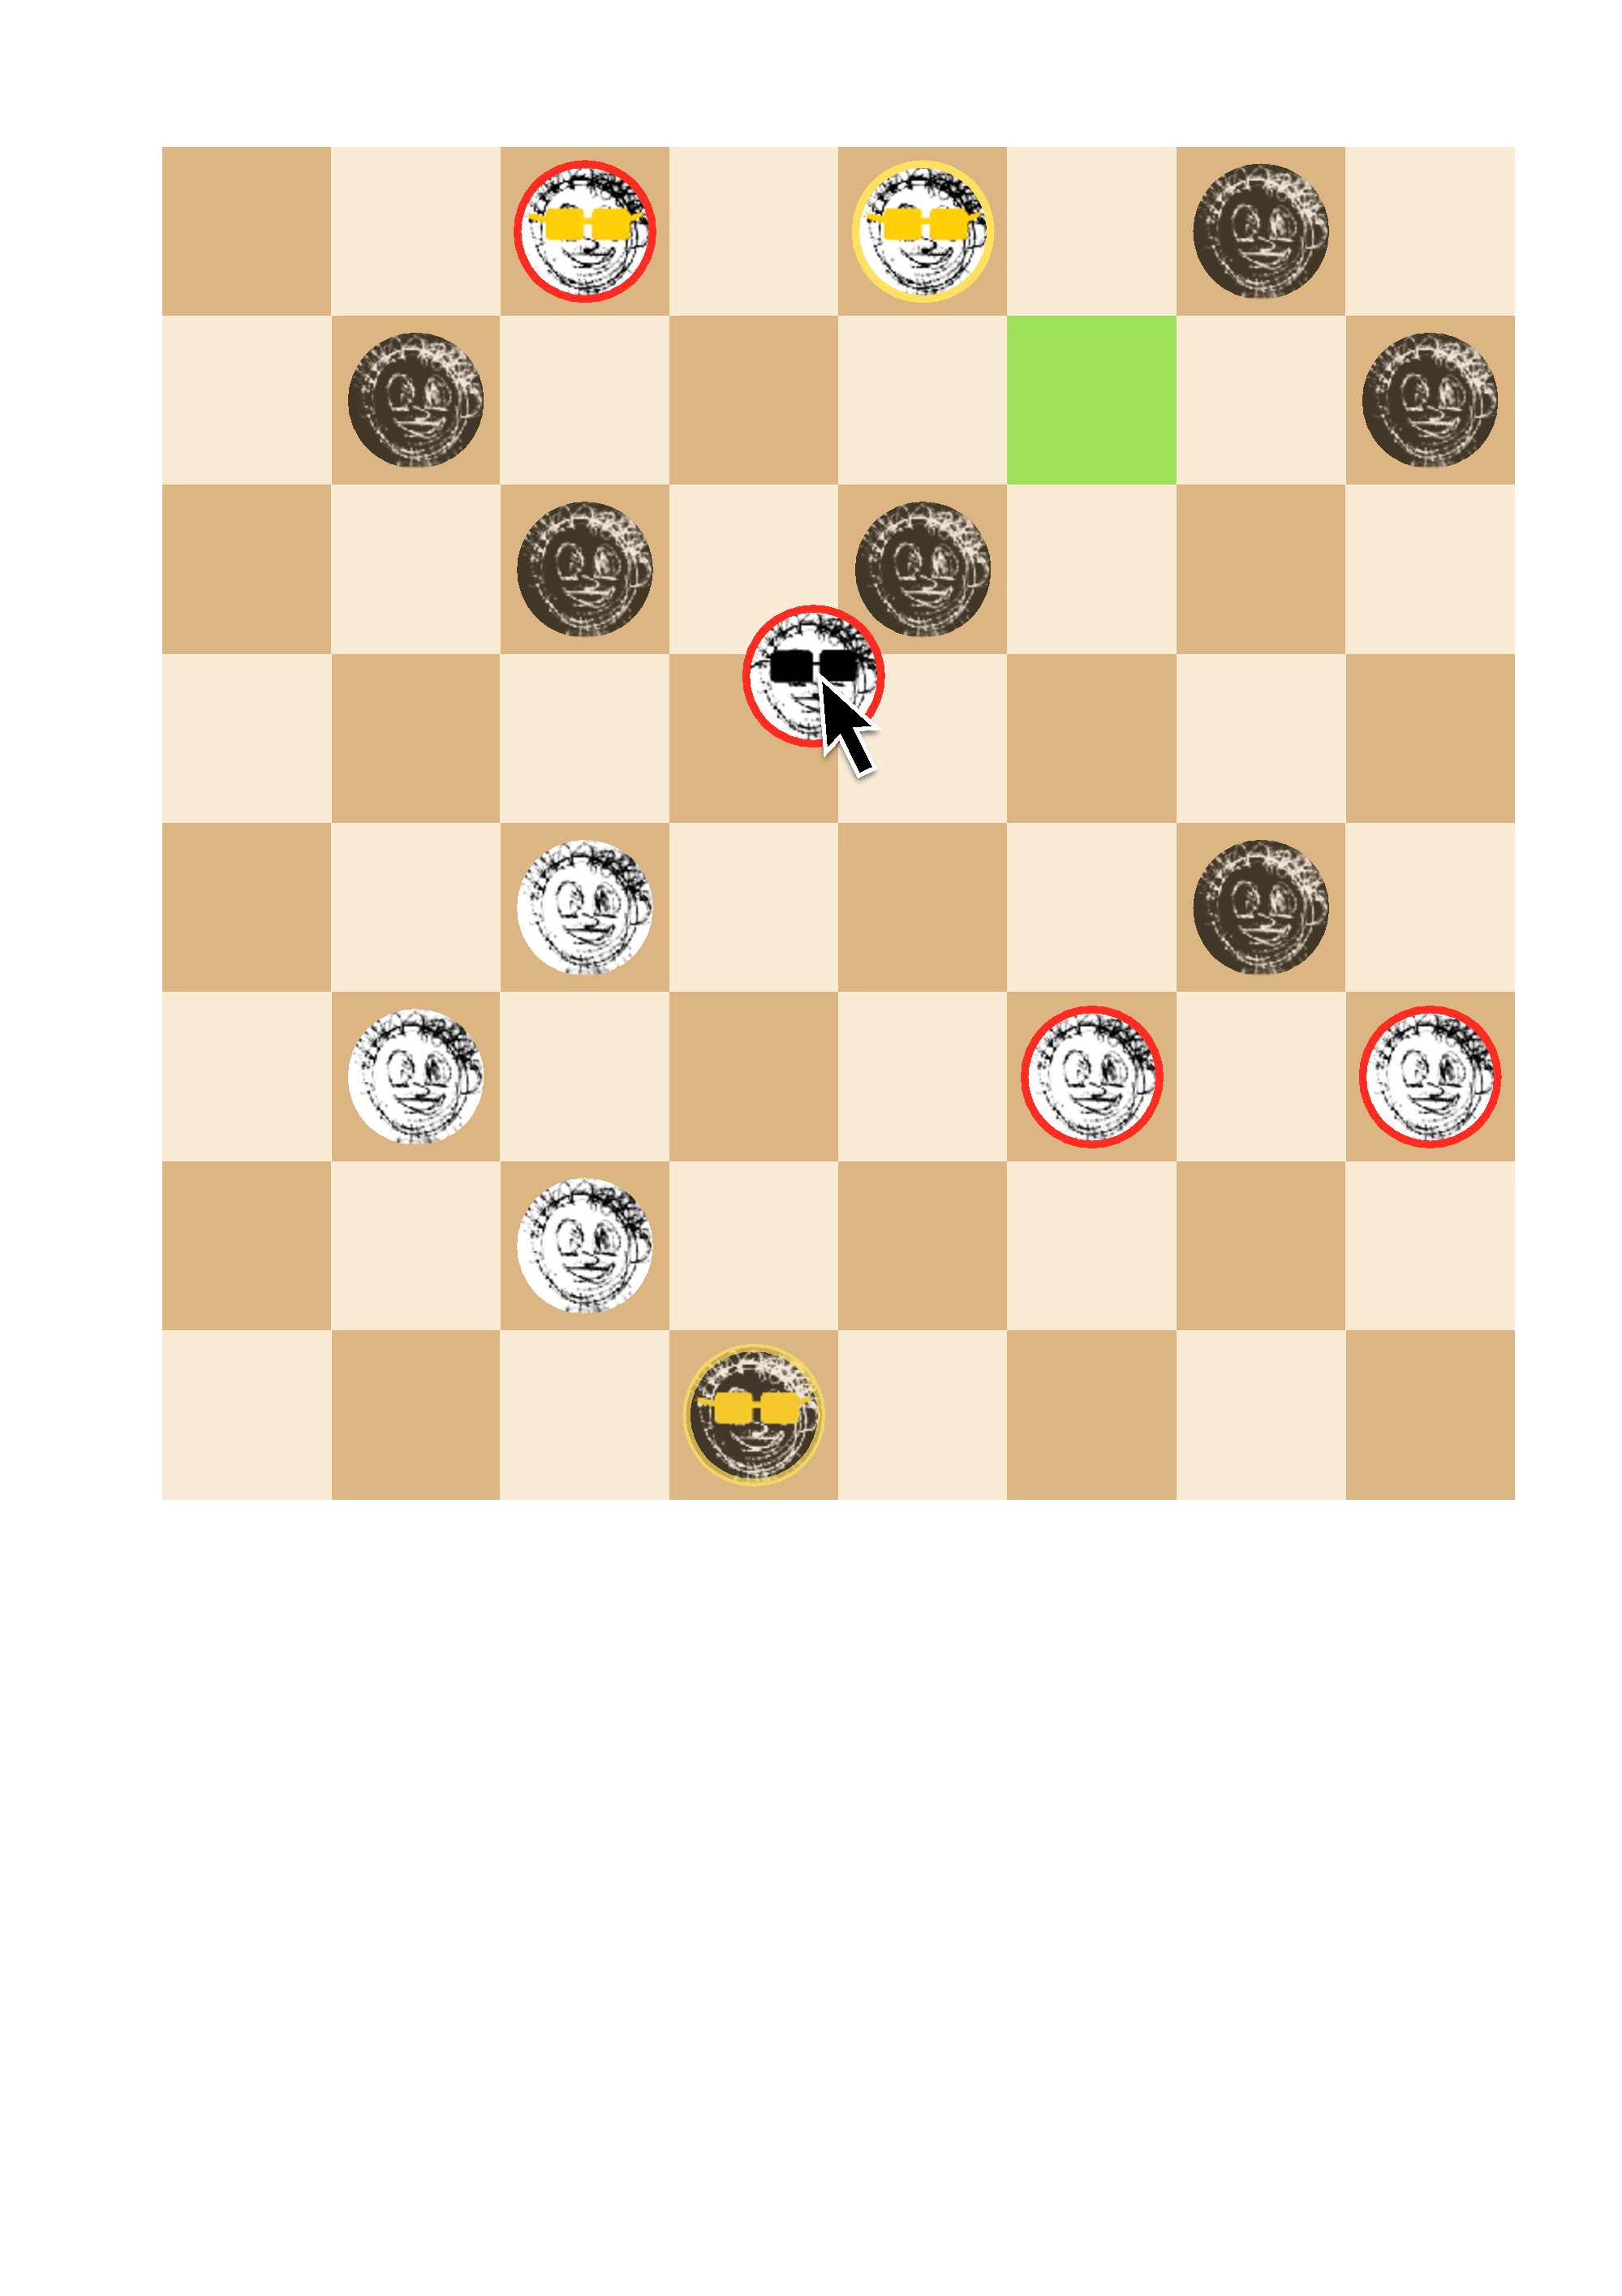
\includegraphics[width = 0.8\textwidth]{Figurer/Forside}
\end{figure}

\vspace{0.5 cm}

\begin{figure}[H]
    \centering
    
\includegraphics{Figurer/DTU3CMYK.eps}
\end{figure}

\pagenumbering{gobble}

\newpage
\section*{Abstract}
This paper describes a way to create a game of Checkers using \texttt{Java} and \texttt{JavaFX} for GUI and user input. In order to achieve this, two different versions of checkers were created, one simple and one advanced. Fundamentally, these two versions are quite similar, but the advanced version has far more features, and a more advanced code structure. First the functionalities are described, followed by details on how they were designed and implemented in both versions of the game. Finally, additional features that could have been implemented are listed.
%\section{Spørgsmål}


%\subsection{Spørgsmål: implementering}
%\begin{itemize}
%    \item Hvor ens er SimpDam og AvanceretDam? (overordnet) \CT 
    
%    \item Hvad har I gjort for at gøre spillet flydende/smooth at spille? (adv dam) \CT
    
%    \item Hvor mange ressourcer kræver spillet? (overordnet/begge)\CT
    
%    \item Hvordan håndhæver I model-view-control? (overordnet/begge)\CT
    
%    \item Hvilken platform har I brugt til view? (Swing, JavaFX) (overordnet) \CT
    
%    \item Hvordan håndteres FPS? (overordnet) \CT
    
%    \item Hvilke classes bruger spillet? simp \CT adv \CT 
    
%    \item Hvordan bruges I styles og CSS? (adv) \CT
    
%    \item Hvorfor instansierer I ikke så mange objekter? (overordnet) \CT
    
%    \item Hvorfor har View så meget kontrol? (MouseEvents) (overordnet/begge) \CT
    
%    \item Hvorfor er alt static? (overordnet/begge) \CT
    
%    \item Hvorfor er modellen et field i view klassen? (adv) \CT
    
%    \item Hvordan håndteres scenes? (adv) \CT
    
%    \item Er felterne knapper eller andre objekter? (begge) \CT
    
%    \item Hvorfor bruger I JavaFX shapes i modellen? (overordnet/begge) \CT
       
%    \item Hvordan håndteres user input? (musse klik) (simp) \CT (adv) \CT
    
%    \item Hvordan lagres brikker og tiles internt? (model) (simp) \CT (adv) \CT
    
%    \item Hvordan markeres kongebrikker? Billeder på billeder, eller udskift? (advdam) \CT
    
%    \item Hvordan og hvornår opdateres modellen? (simp) \CT (adv) \CT 
    
%    \item Hvordan lagres spillereglerne? (adv) \CT
    
%    \item Hvordan laves (spawnes) bræt og brikker? (simp) \CT (adv) \CT
    
%    \item Hvordan snappes brikker til tiles? (visuelt) (overordnet) \CT
    
%    \item Hvordan dræbes brikker? Bliver de slettet eller skjult? (simp) \CT (adv) \C
    
%    \item Hvordan dræbes fjender i comboer? (adv) \CT
    
%    \item Hvilke fields og methods bruges ved comboer? (adv) \CT
    
%    \item Hvordan håndteres, hvilke brikker, der må dræbes? (begge) \CT
    
%    \item Hvordan startes spillet? (method calls) (simp) \CT (adv) \CT
    
%    \item Hvordan sluttes spillet? (vinder, tie) (begge) \CT
    
%    \item Hvordan afgør spillet, at nogen har vundet? (adv) \CT 
    
%    \item Hvordan styres, hvis tur det er? (overordnet) \CT 
    
%    \item Hvordan afholder I den "forkerte" spiller fra at trække, når det ikke er deres tur? (overordnet/begge) \CT 
    
%    \item Hvordan styres et helt træk med en brik? (TLC, control, method calls). (simp) \CT (adv) \CT
    
%    \item Hvordan highlightes felter? (adv) \CT
    
%    \item Hvordan håndteres og opdateres score labels? (adv) \CT
    
%    \item Hvordan tilpasses billeder til brikken? (adv) \CT
    
%    \item Hvad sker der, hvis vi uploader et stort billede? (adv) \CT
    
%    \item Hvordan navngiver I methods og variable? (overordnet) \CT
    
%    \item Hvordan har I struktureret koden, så den er læsbar for andre? (overordnet) \CT
    
%    \item Hvordan håndteres abstraktionsniveau i kontrollen? (overordnet) \CT
    
%    \item Hvad er TopLevelControl? (overordnet/begge) \CT
    
%    \item Hvordan ved læseren af koden, hvordan en method virker/bruges? (comments) (overordnet) \CT
    
%    \item Hvordan sørger I for, at brikker ikke bevæger sig uden for brættet? (begge) \CT
    
%    \item Hvordan er save og load implementeret? (adv) \CT
    
   % \item Hvordan lagres data i en save file? (adv) \CT
    
  %  \item Hvordan forhindres fejl loading? (load uden save file) (adv) \CT
    
%    \item Hvordan skiftes mellem billeder af ikke-fokus brik, valgt brik, og kronet brik? (adv) \CT
    
%    \item Hvordan er rød og guld ring implementeret? (adv) \CT
    
%    \item Hvordan animeres spawn og død? (adv) \CT
    
%    \item Hvordan animeres flytning af brik? (adv, begge?) \CT
    
 %   \item Hvordan animeres AI flytning af brik? (adv) \CT
    
%    \item Hvordan animeres AI flytning af comboer? (adv) \CT
    
%    \item Hvor mange ressourcer bruger AI? (adv) \CT
    
%    \item Hvor hurtigt tager AI et træk? (adv) \CT
    
%     \item Hvad sker der når der skiftes tur? (simp) \CT (adv) \CT
    
%\end{itemize}

\subsection{Spørgsmål: evaluering}
\begin{itemize}
%    \item Hvordan endte I med den program struktur, I har? (historie om highlights) \CT
%    \item Hvordan holdt I styr på projektet? (Hvad er gjort, hvad skal implementeres, debugges). Logbog. \CT
%    \item Hvordan håndterede I versionskontrol? \CT
%    \item Debugging: Hvor sikkert er spillet? Hvilke sanisations har I på inputs? \CT
%    \item Hvad ville I implementere/debugge/forfine, hvis I havde mere tid? \CT
\end{itemize}

















%\section{Figurer}
\subsection{Figurer: design}

\begin{itemize}
    \item Figur med drag: smooth.
    
    \item Billeder/figur af brikker med ringe om: mandatoryKill(rød), crowned (gul) og en 30 \% gennemsigtig brik. Til design afsnit om visuelle indikatorer
    
    \item Highlight alm. træk.
    
    \begin{figure}[H]
        \centering
        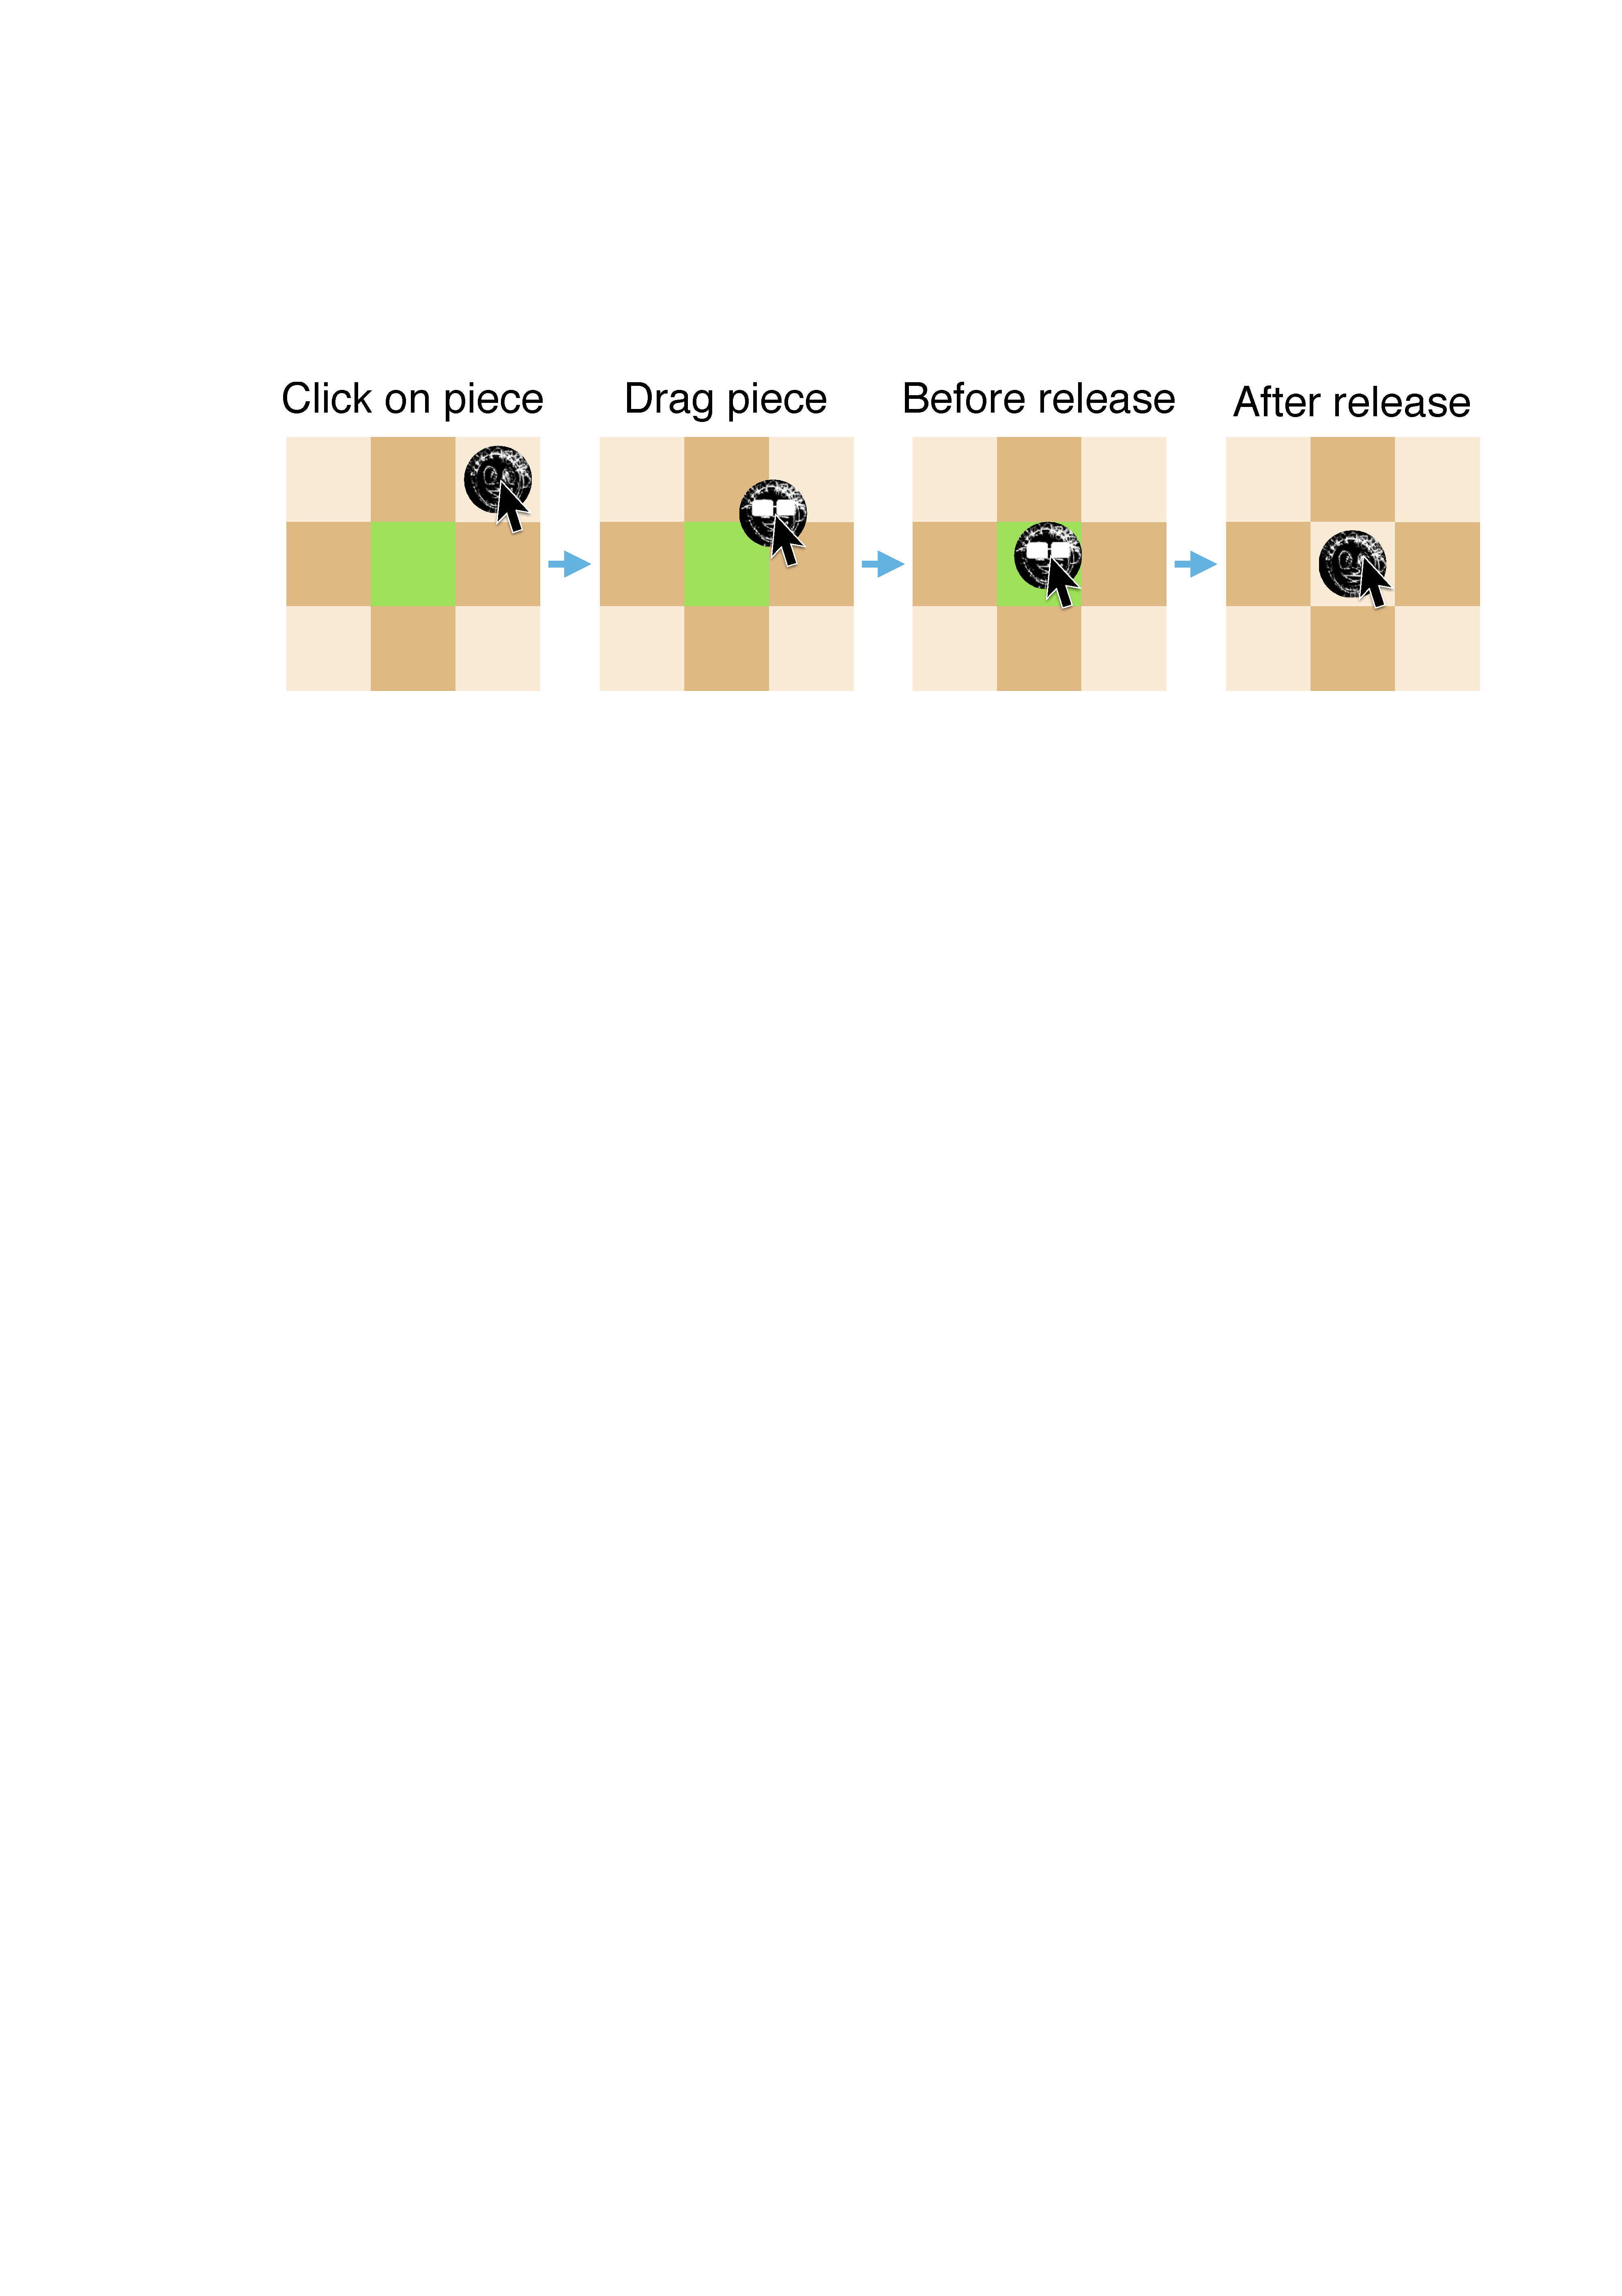
\includegraphics[width = \textwidth]{Figurer/MovePieceFigure}
        \caption{Caption}
        \label{fig:MovePieceFigure}
    \end{figure}

    \item Highlight combo.
    
    \begin{figure}[H]
        \centering
        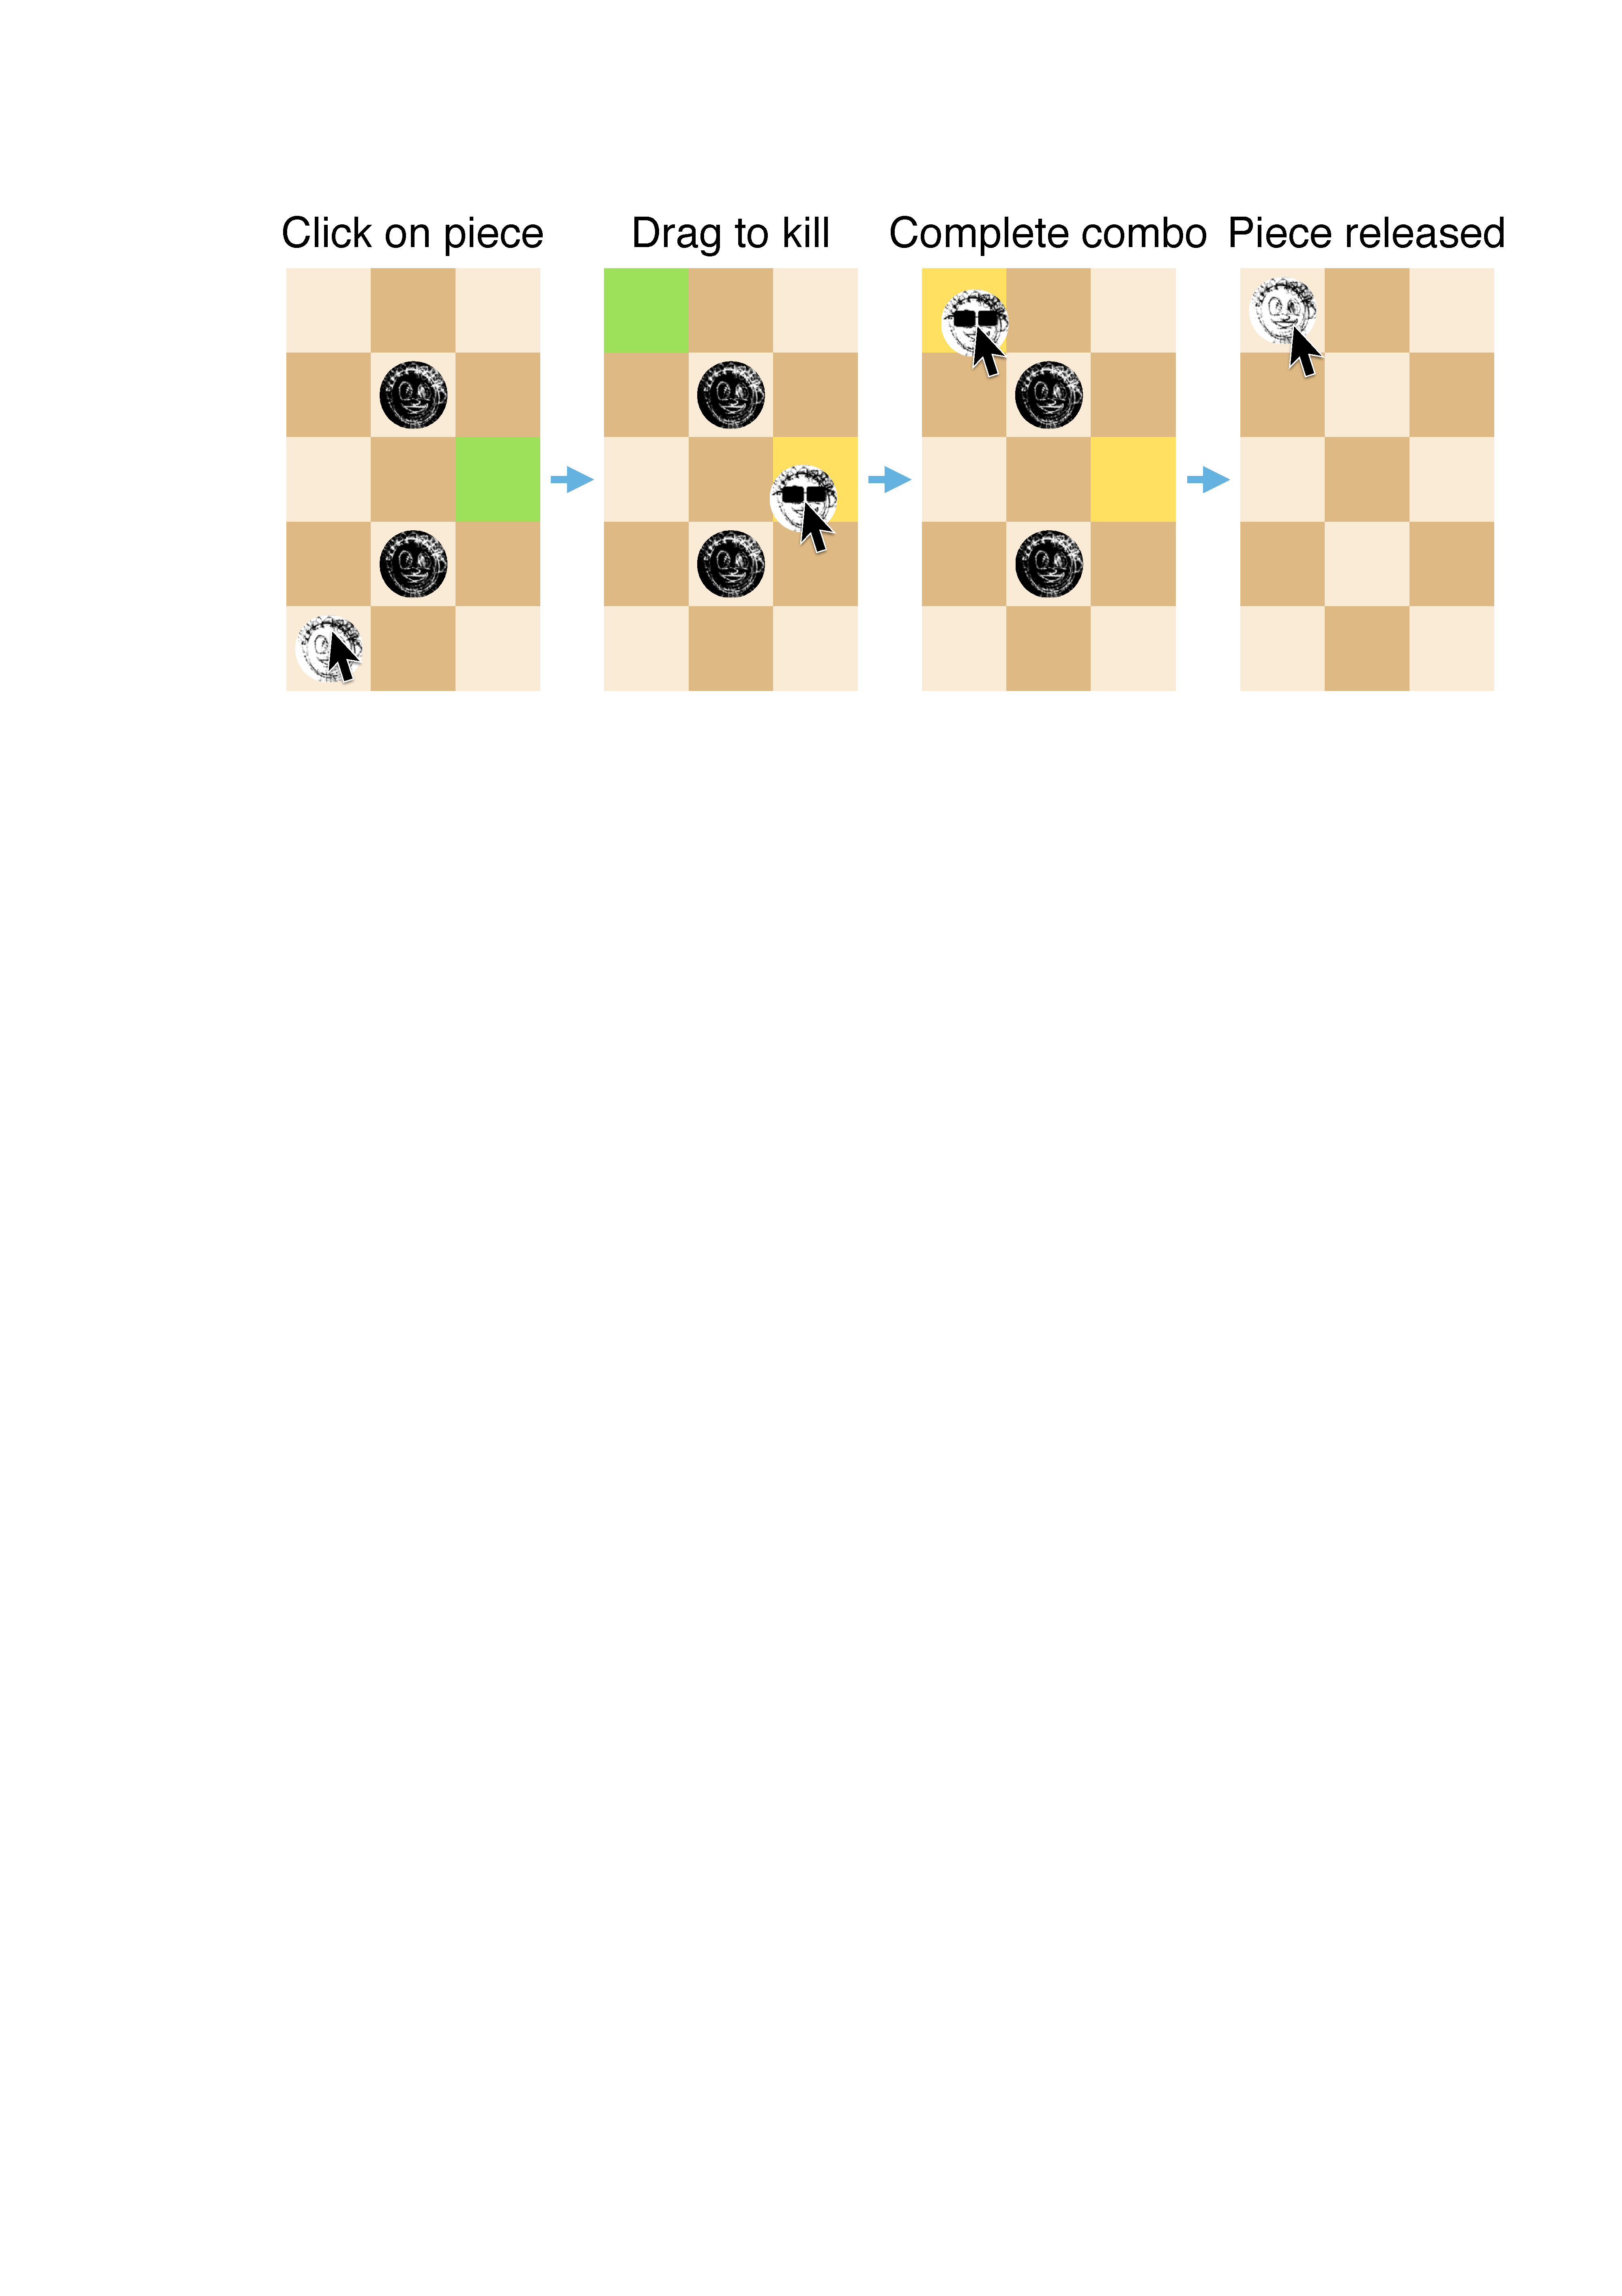
\includegraphics[width = \textwidth]{Figurer/ComboFigure}
        \caption{Caption}
        \label{fig:ComboFigure}
    \end{figure}
    
    \item Klasse diagrammer.
    
    \begin{figure}[H]
        \centering
        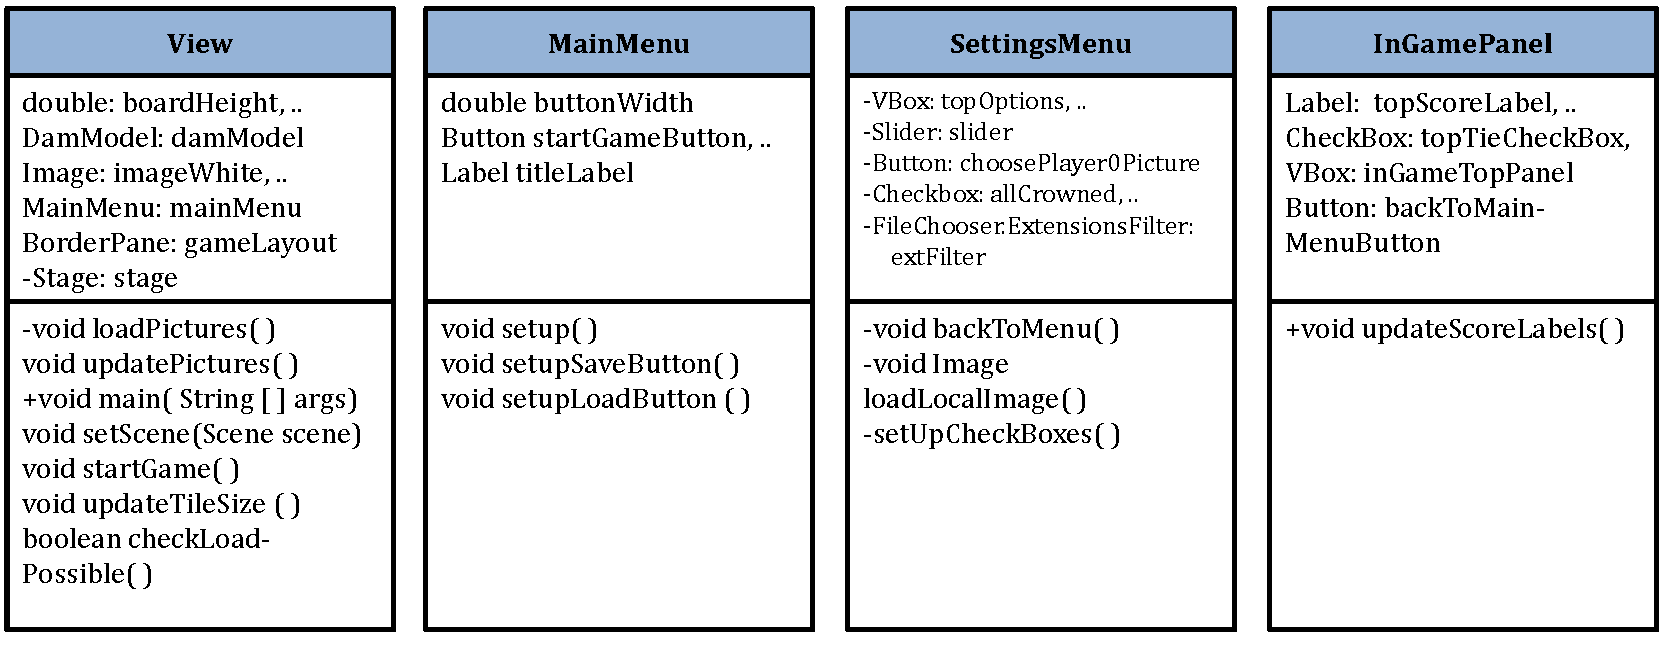
\includegraphics[width = 0.4  \textwidth]{Figurer/classesView.pdf}
        \caption{Caption}
        \label{fig:classesView}
    \end{figure}
    
       \begin{figure}[H]
        \centering
        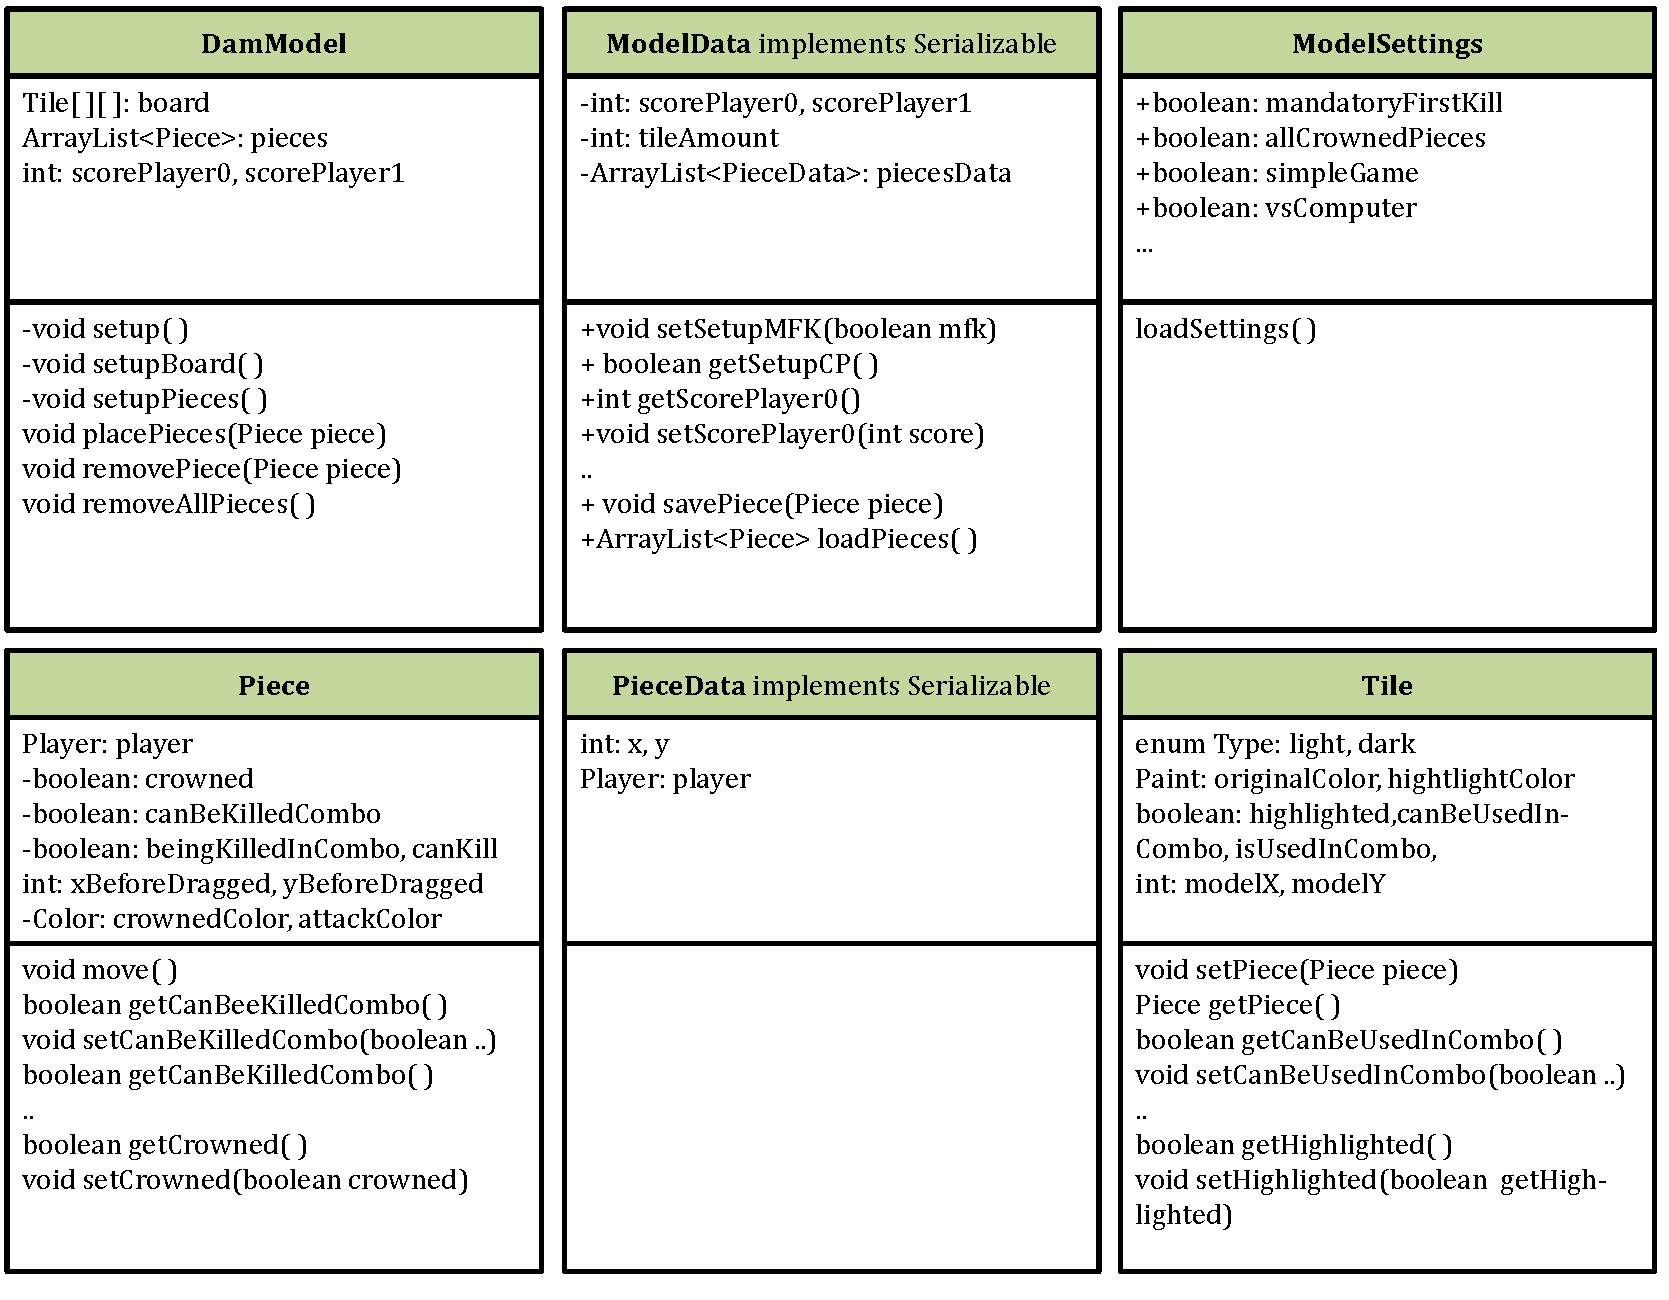
\includegraphics[width = 0.4  \textwidth]{Figurer/classesModel.pdf}
        \caption{Caption}
        \label{fig:classesModel}
    \end{figure}
    
       \begin{figure}[H]
        \centering
        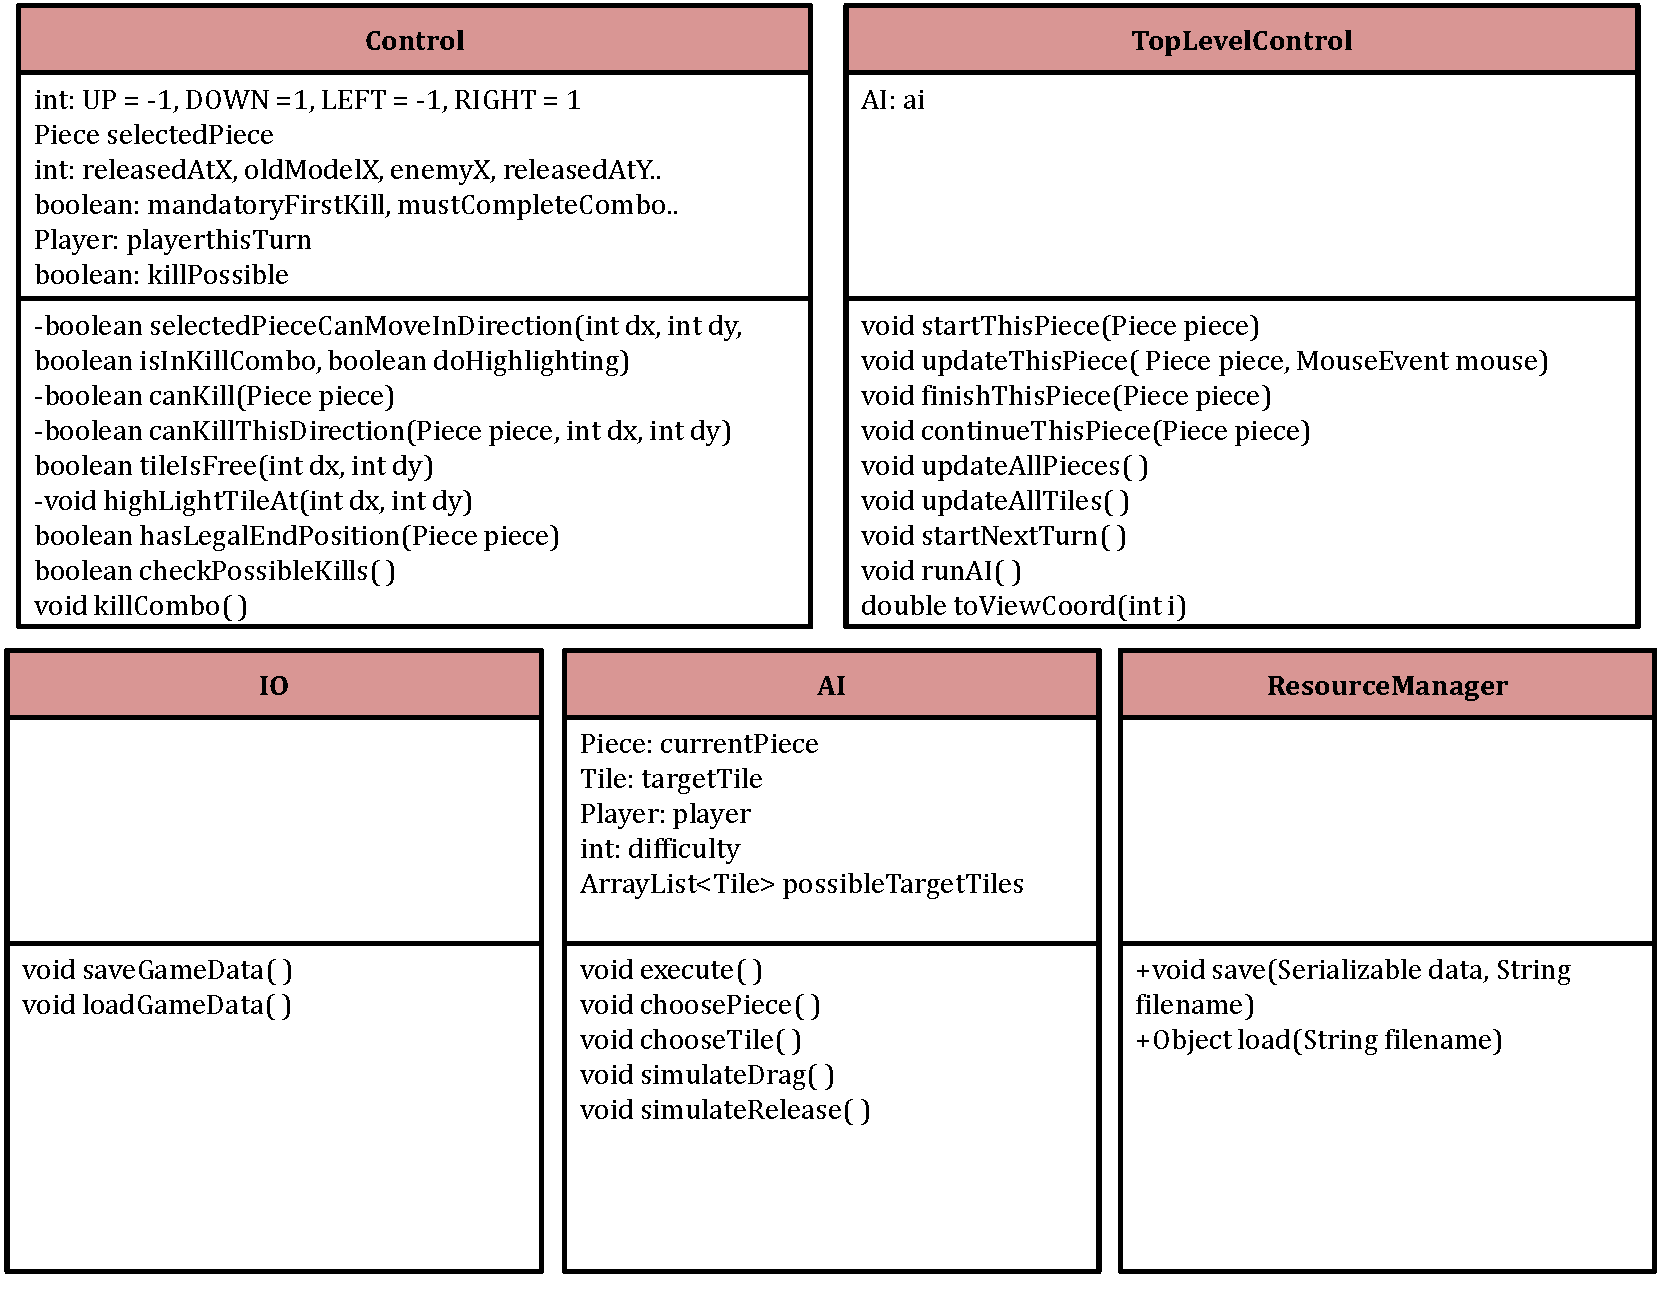
\includegraphics[width = 0.4  \textwidth]{Figurer/classesControl.pdf}
        \caption{Caption}
        \label{fig:classesControl}
    \end{figure}
    
    \item Model view control.
    
    \begin{figure}[H]
        \centering
        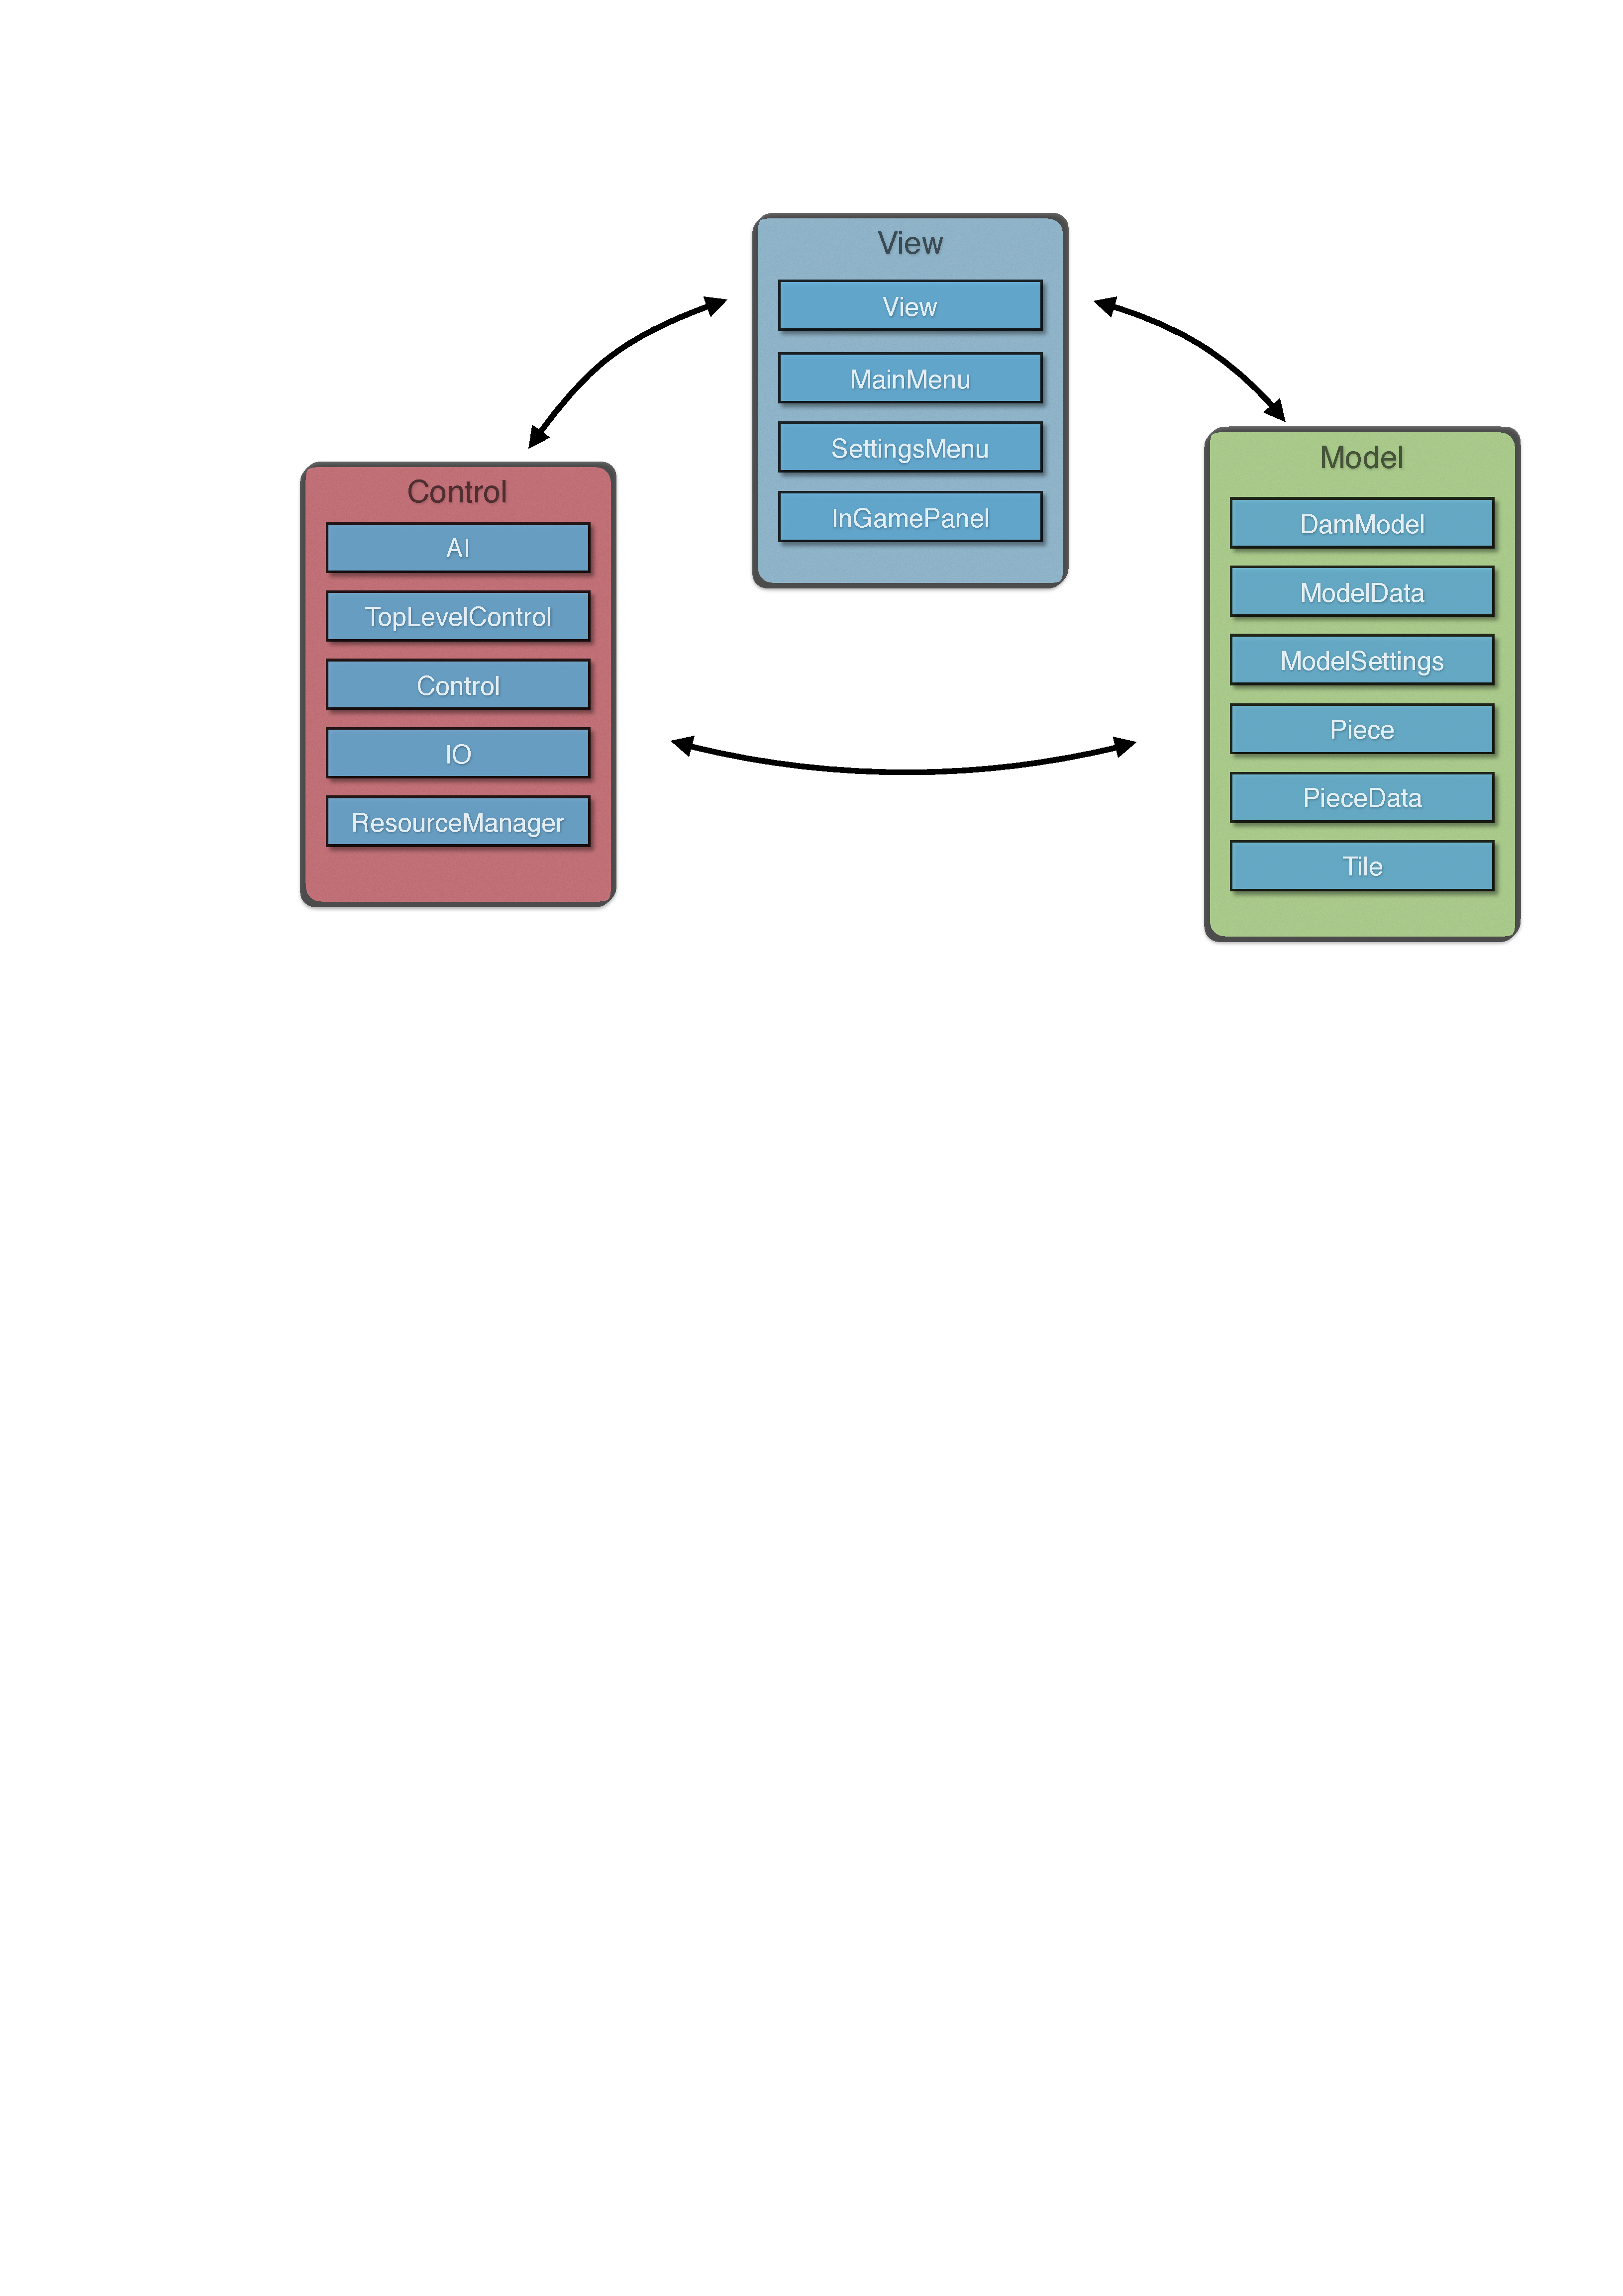
\includegraphics[width = 0.4 \textwidth]{Figurer/Model-View-Control}
        \caption{Caption}
        \label{fig:MVC}
    \end{figure}
    
    \begin{figure}[H]
        \centering
        \includegraphics[width = 0.4\textwidth]{Figurer/DefaultPieces}
        \caption{Caption}
        \label{fig:defaultPieces}
    \end{figure}

\item Start spil.
    \begin{figure}[H]
        \centering
        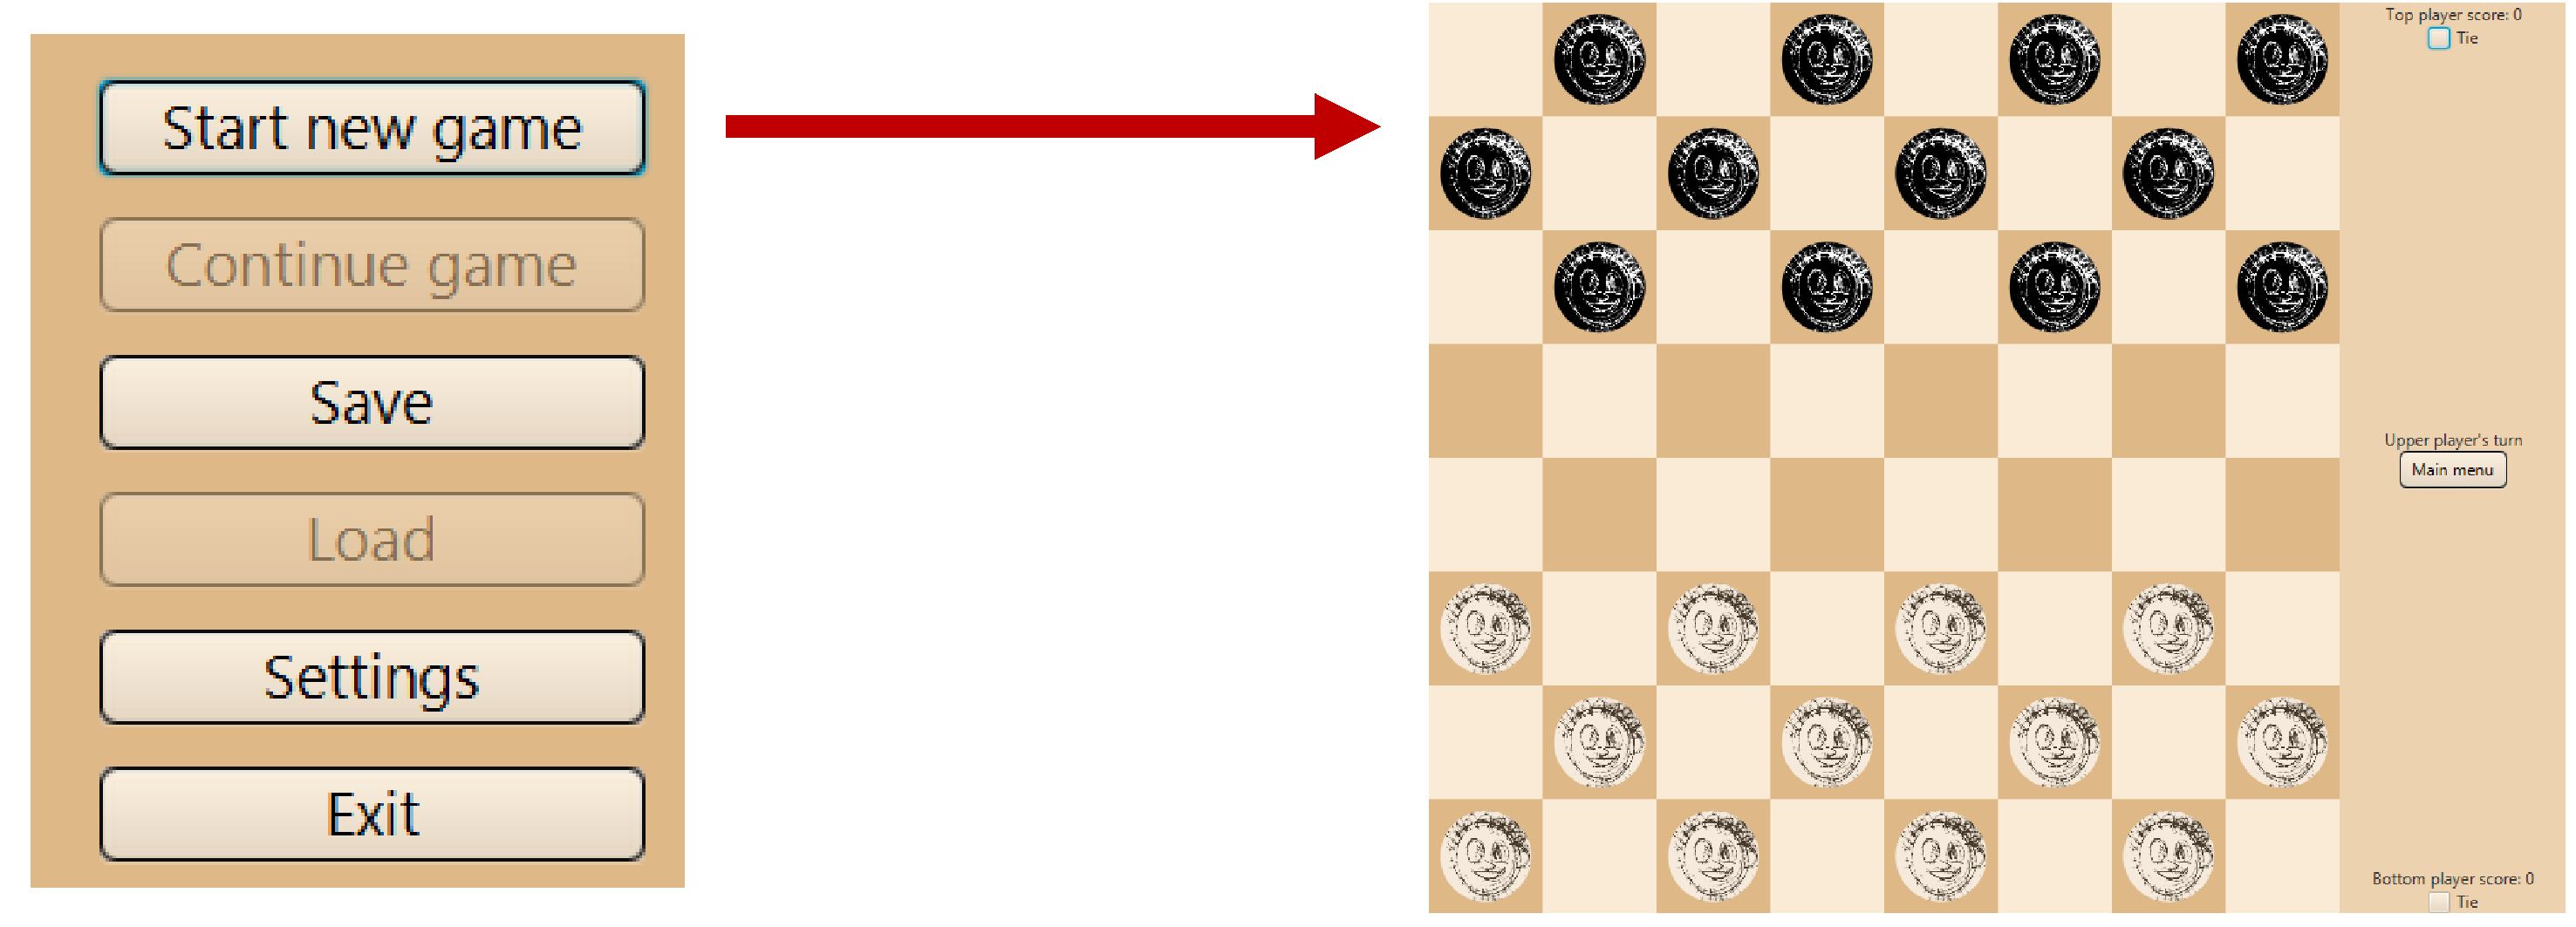
\includegraphics[width = 0.4  \textwidth]{Figurer/gameStart}
        \caption{Caption}
        \label{fig:gameStart}
    \end{figure}
\end{itemize}

\subsection{Figurer: implementering}

\begin{itemize}
    \item Control flow med methods.
\end{itemize}


\tableofcontents

\newpage
\pagenumbering{arabic}
\setcounter{page}{1}
\section{Ansvarsoversigt}
\vspace{-0.5cm}
\begin{figure}[H]
\centering
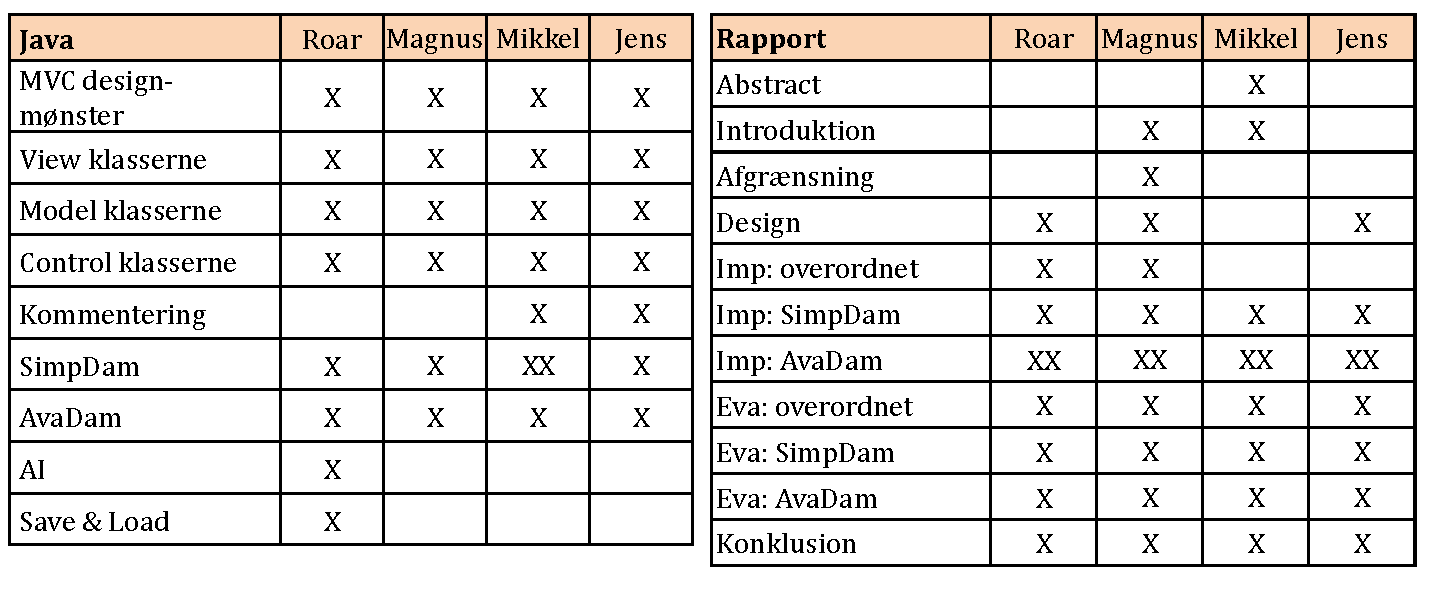
\includegraphics[width = 1.0\textwidth]{Figurer/ansvarsOversigt.pdf}
%\caption{Caption}
\label{fig:ansvarsOversigt}
    \end{figure}
    
\vspace{-0.5cm}
\section{Introduktion}

% Magnus
% Into, der svarer til deres intro omskrevet
I denne rapport dokumenterer vi designet og implementeringen af vores computerspil baseret på det klassiske brætspil dam. Der er forskellige regelsæt for dam, så vi tog udgangspunkt i reglerne fra Wikipedia\footnote{Wikipedia: \url{https://da.wikipedia.org/wiki/Dam_(br\%C3\%A6tspil)}} og Dansk Dam Forening\footnote{Dansk Dam:  \url{http://www.danskdam.dk/}}. De fleste implementerede regler er aktiverbare gennem en menu i spillet.\\

Vi har to endelige versioner af spillet: \\
\textbf{\textsc{SimpDam}:} En simpel version af dam med kun én brik til hver spiller og få regler. Brættets størrelse er skalérbart.\\

\textbf{\textsc{AvaDam}:} Et mere avanceret damspil med aktivérbare regler, et skalérbart brætstørrelse, animationer og features som highlights, comboer, spil mod computer og save/load.\\

\textbf{Struktur af rapport:} Af hensyn til læseren er rapporten struktureret, så design og implementering af \textsc{SimpDam} og \textsc{AvaDam} gennemgås separat. \textsc{AvaDam} bygger dog videre på \textsc{SimpDam}, så hvert kapitel indledes med et fælles afsnit. Vi har forsøgt at anvende model-view-control designmønstret under projektforløbet; dette ses også i rapportens opbygning. \\

%% MIKKEL %%
% Hvem er spillets målgruppe?
\textbf{Spillets målgruppe:} Vores dam spil er sat op til at være intuitivt at kontrollere og reglerne lette at tyde. Dette er gjort, så det henvender sig bedre til den forholdsvis nye dam-spiller, der allerede kender de basale regler. Spilleren har ikke nødvendigvis helt overblik over hvordan alle reglerne hænger samme, og der er derfor skabt en intuitiv brugergrænseflade der fortællere spilleren, på en simpel måde, hvilke mulige træk en given brik har. Vores spil henvender sig også til spilleren der ikke altid har nogen at spille sammen med, og har derfor implementeret en AI. Denne er lavet til ikke at være så udfordrende, da spillets målgruppe ikke er mester til dam.

\section{Afgrænsning}\label{sec:afgraensning}

% Magnus
\subsection{Grundlæggende del: \textsc{SimpDam}}
I den grundlæggende del konstruerede vi et simpelt damspil, hvor interaktionen med brugerne foregår via en grafisk brugergrænseflade implementeret med \texttt{JavaFX}. Brætstørrelsen $n \in \{3, .. , 100\}$ sættes af brugeren. Vi har vedhæftet to udgaver af \textsc{SimpDam}: En \texttt{.jar}-fil, hvor $n$ angives som en kommandolinjeparameter, når \texttt{.jar}-filen køres gennem terminalen. Samt en \texttt{Eclipse} projektfil med dertilhørende \texttt{.java}-filer, hvor $n$ efterspørges gennem konsollen i \texttt{Eclipse}.

% Magnus
\subsection{Avanceret del: \textsc{AvaDam}}

Det avancerede damspil har samme grundstruktur som det simple damspil, men vi har udvidet med en del ekstra features. De mest væsentlige features findes på figurerne \ref{fig:features1} og \ref{fig:features2}, og uddybes i afsnittene Design og Implementering. \\
\begin{figure}[H]
\centering
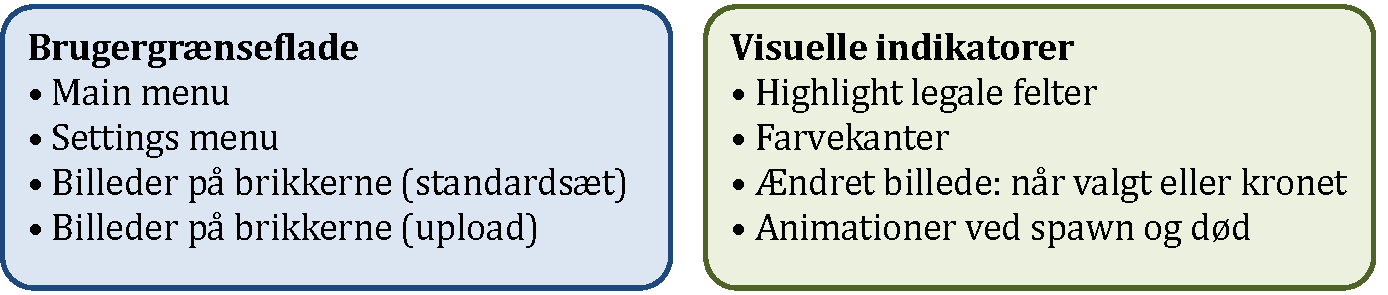
\includegraphics[width = 1.0  \textwidth]{Figurer/features1.pdf}
\caption{Yderligere implementeringer efter \textsc{SimpDam}. Del 1 af 2.}
\label{fig:features1}
\end{figure}

\begin{figure}[H]
\centering
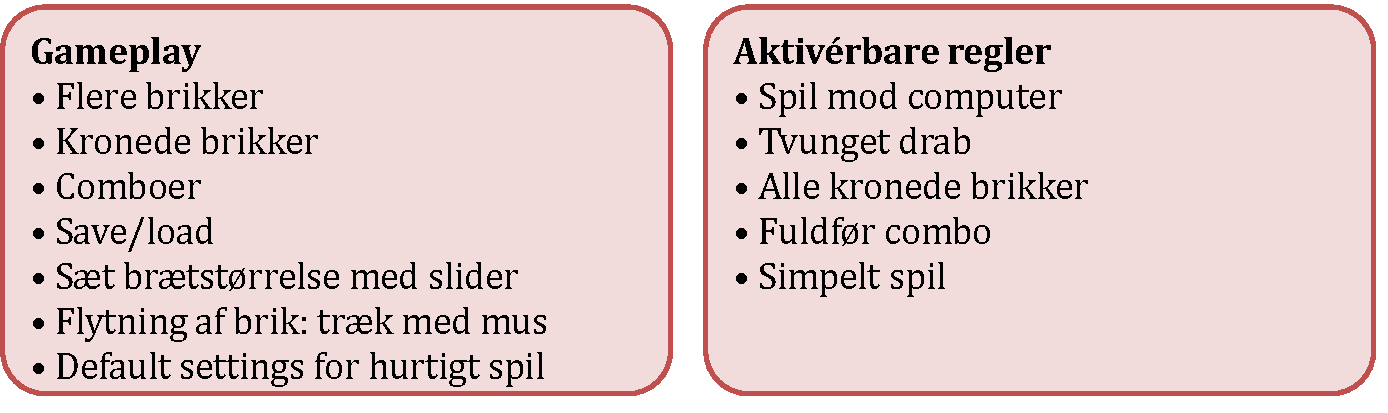
\includegraphics[width = 1.0  \textwidth]{Figurer/features2.pdf}
\caption{Yderligere implementeringer efter \textsc{SimpDam}. Del 2 af 2.}
\label{fig:features2}
\end{figure}


\section{Design}
\subsection{Model-view-control}\label{sec:designMVC}
% RR
%    \item Hvordan håndhæver I model-view-control?
%       &
%    \item Hvorfor har View så meget kontrol? (MouseEvents) ((Mouse events er i Piece tho))

Vi har så vidt muligt opdelt vores spil i de 3 hovedkategorier \textit{model}, \textit{view} og \textit{kontrol}.\footnote{Her tales ikke om specifikke klasser, men abstrakt om model-view-control designmønstret.} View står for at vise spillet i GUI'en og styre størrelsen af den viste GUI. Diverse menu'er er også placeret i view, hvilket gør at bruger input gennem menu'er går gennem view. Modellen består af spillets brikker samt brættet selv med dets felter. Kontrollen fortæller brugeren hvilke træk der kan foretages og tjekker om foretagede træk er gyldige. Selve spil logikken er placeret i kontrol. Én specifik konsekvens af at bruge \texttt{JavaFX} er at man automatisk har overført kontrol til alt der bruger \texttt{Shapes} og \texttt{Nodes}. Dette skyldes event listeners der nødvendigvis er placeret i klasserne selv. Dog er kontrollen styret ved at hver \texttt{Shape} og \texttt{Node} kalder metoder i kontrollen. 

\begin{figure}[H]
\centering
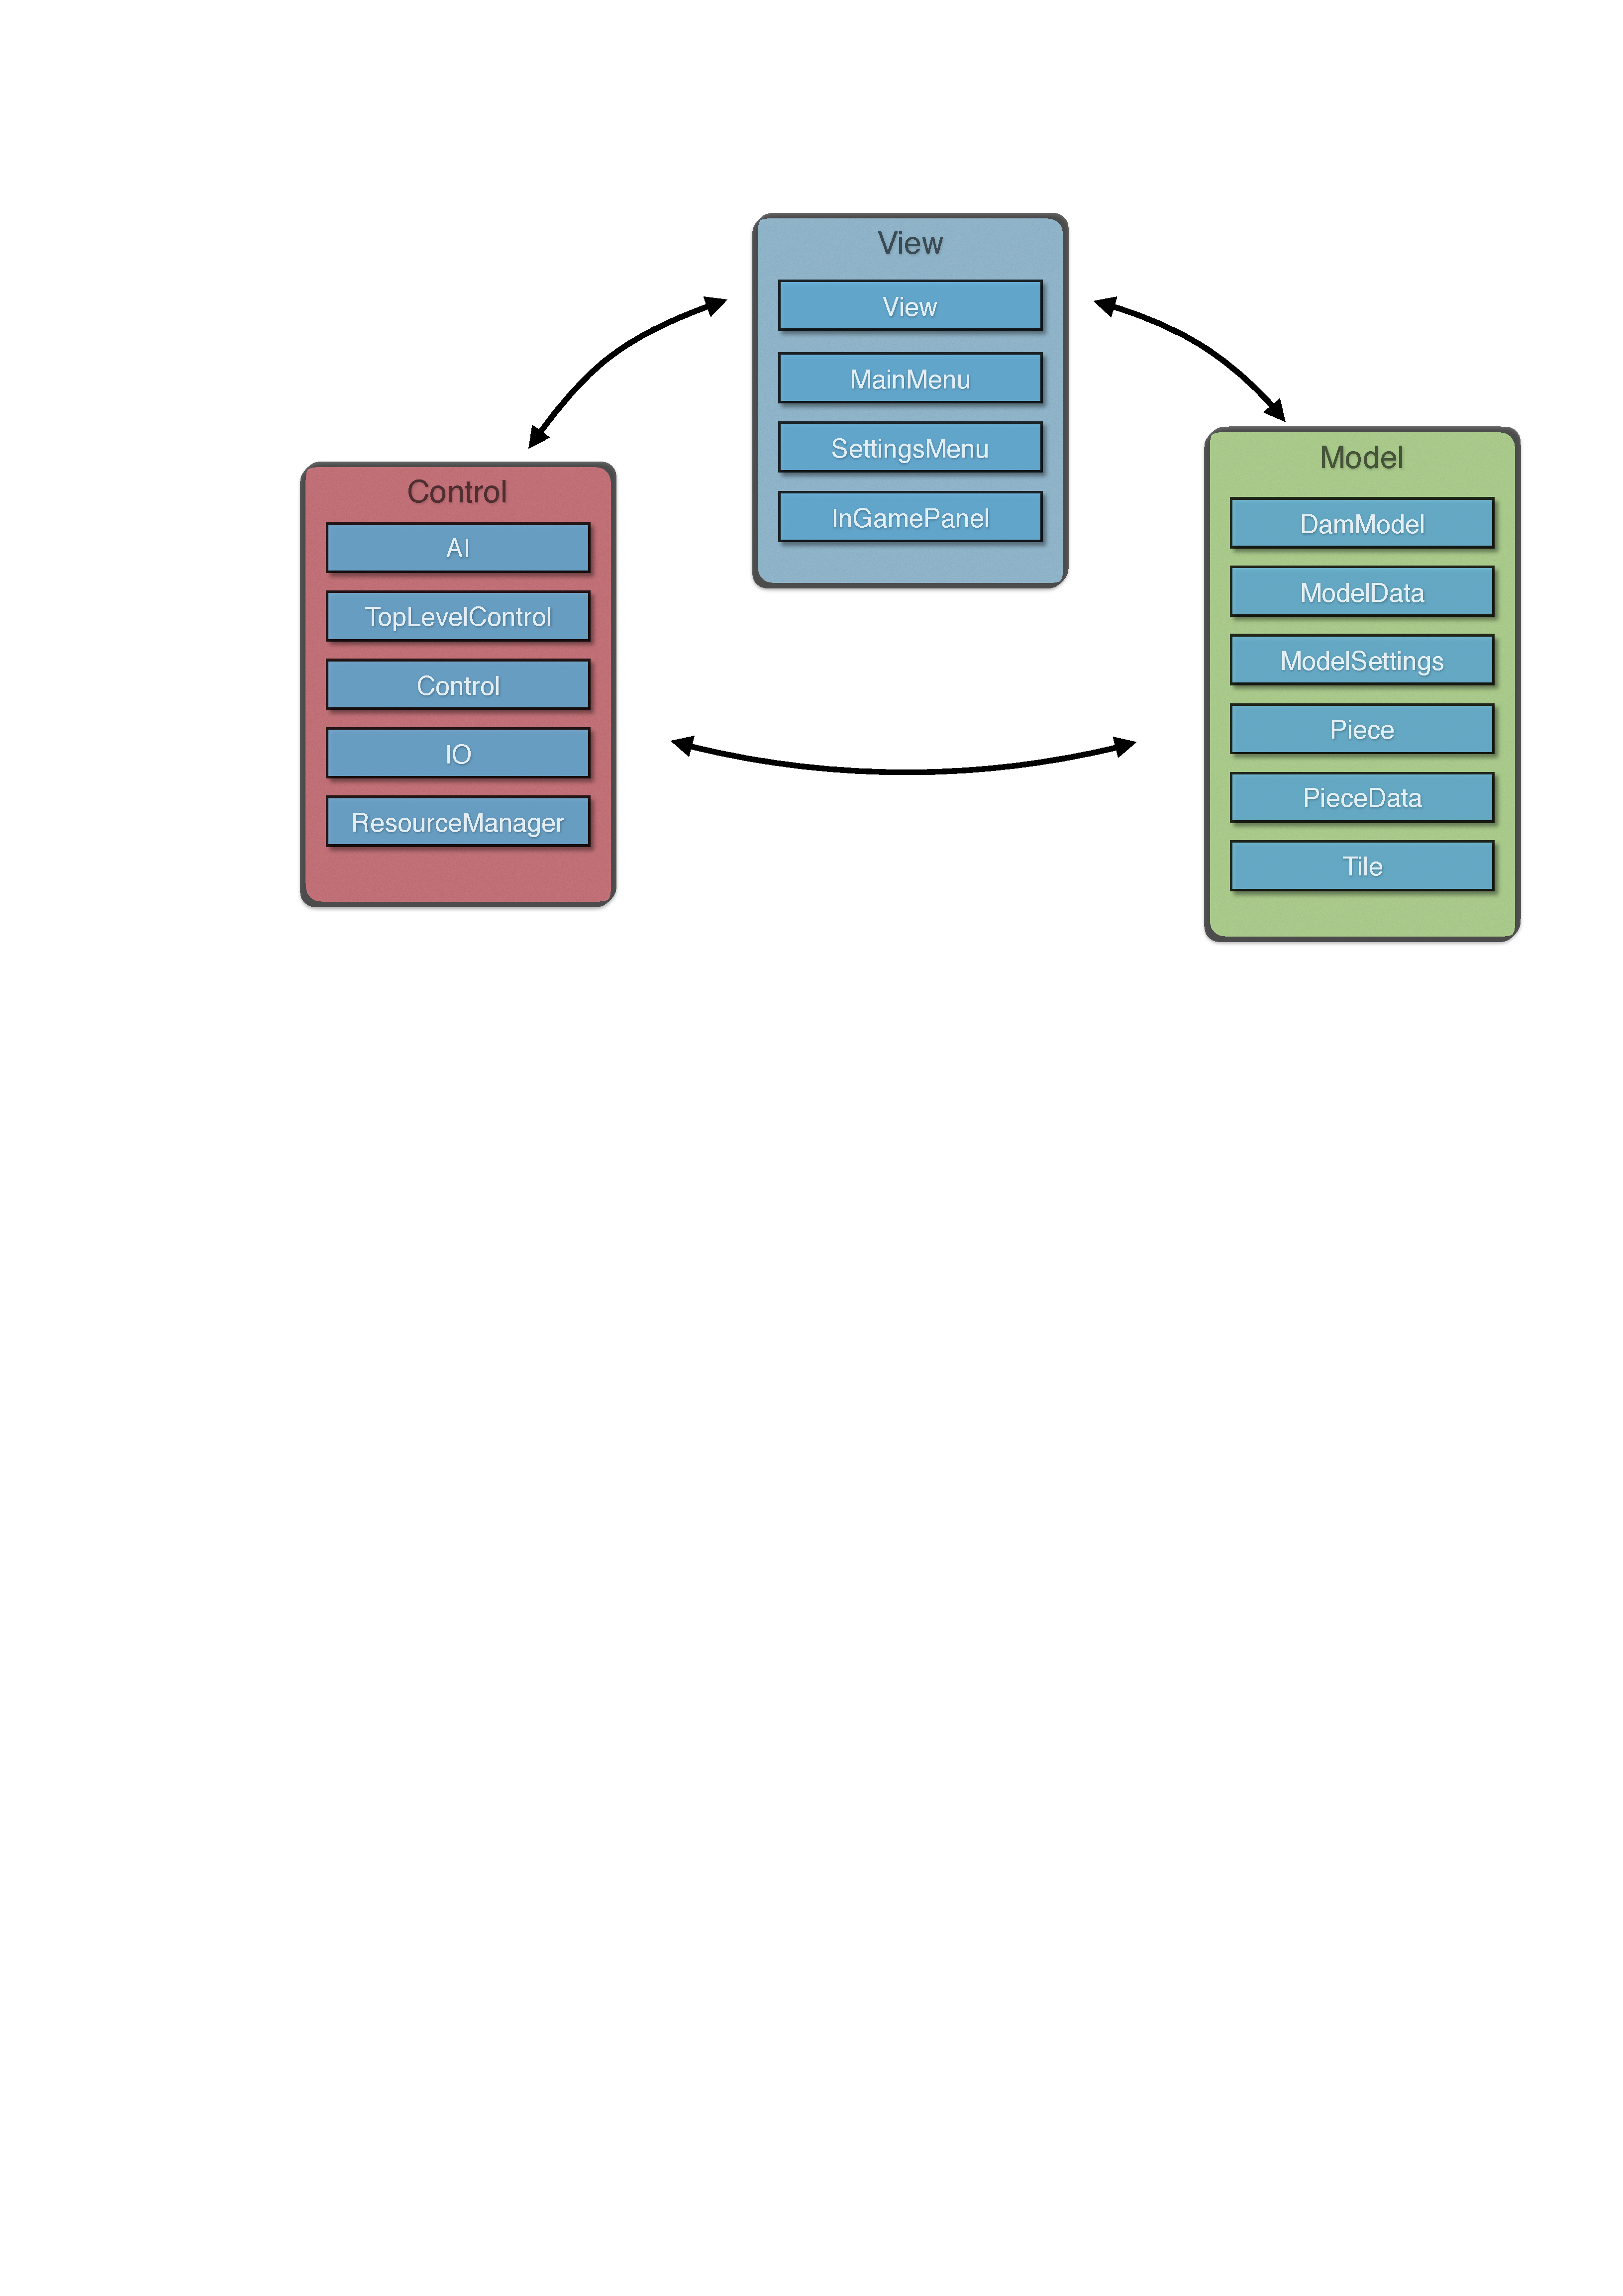
\includegraphics[width = 0.8  \textwidth]{Figurer/Model-View-Control}
\caption{Klasserne der bruges i programmet, delt op efter MVC designmøsntret.}
\label{fig:MVC}
\end{figure}


\subsection{Overordnet}\label{sec:designOverordnet}
% Magnus
% Hvordan startes spillet? 
\textbf{Start:} I \textsc{AvaDam} startes spillet ved at spilleren trykker \texttt{"Start new game"} i main menuen, som set i figur \ref{fig:gameStart}. Derefter oprettes et model objekt i \texttt{View} klassen. Brikker og felter oprettes som objekter af typerne \texttt{Piece} og \texttt{Tile}, der er fields i modelobjektet. I \textsc{SimpDam} startes spillet direkte, når programmet åbnes.

    \begin{figure}[H]
        \centering
        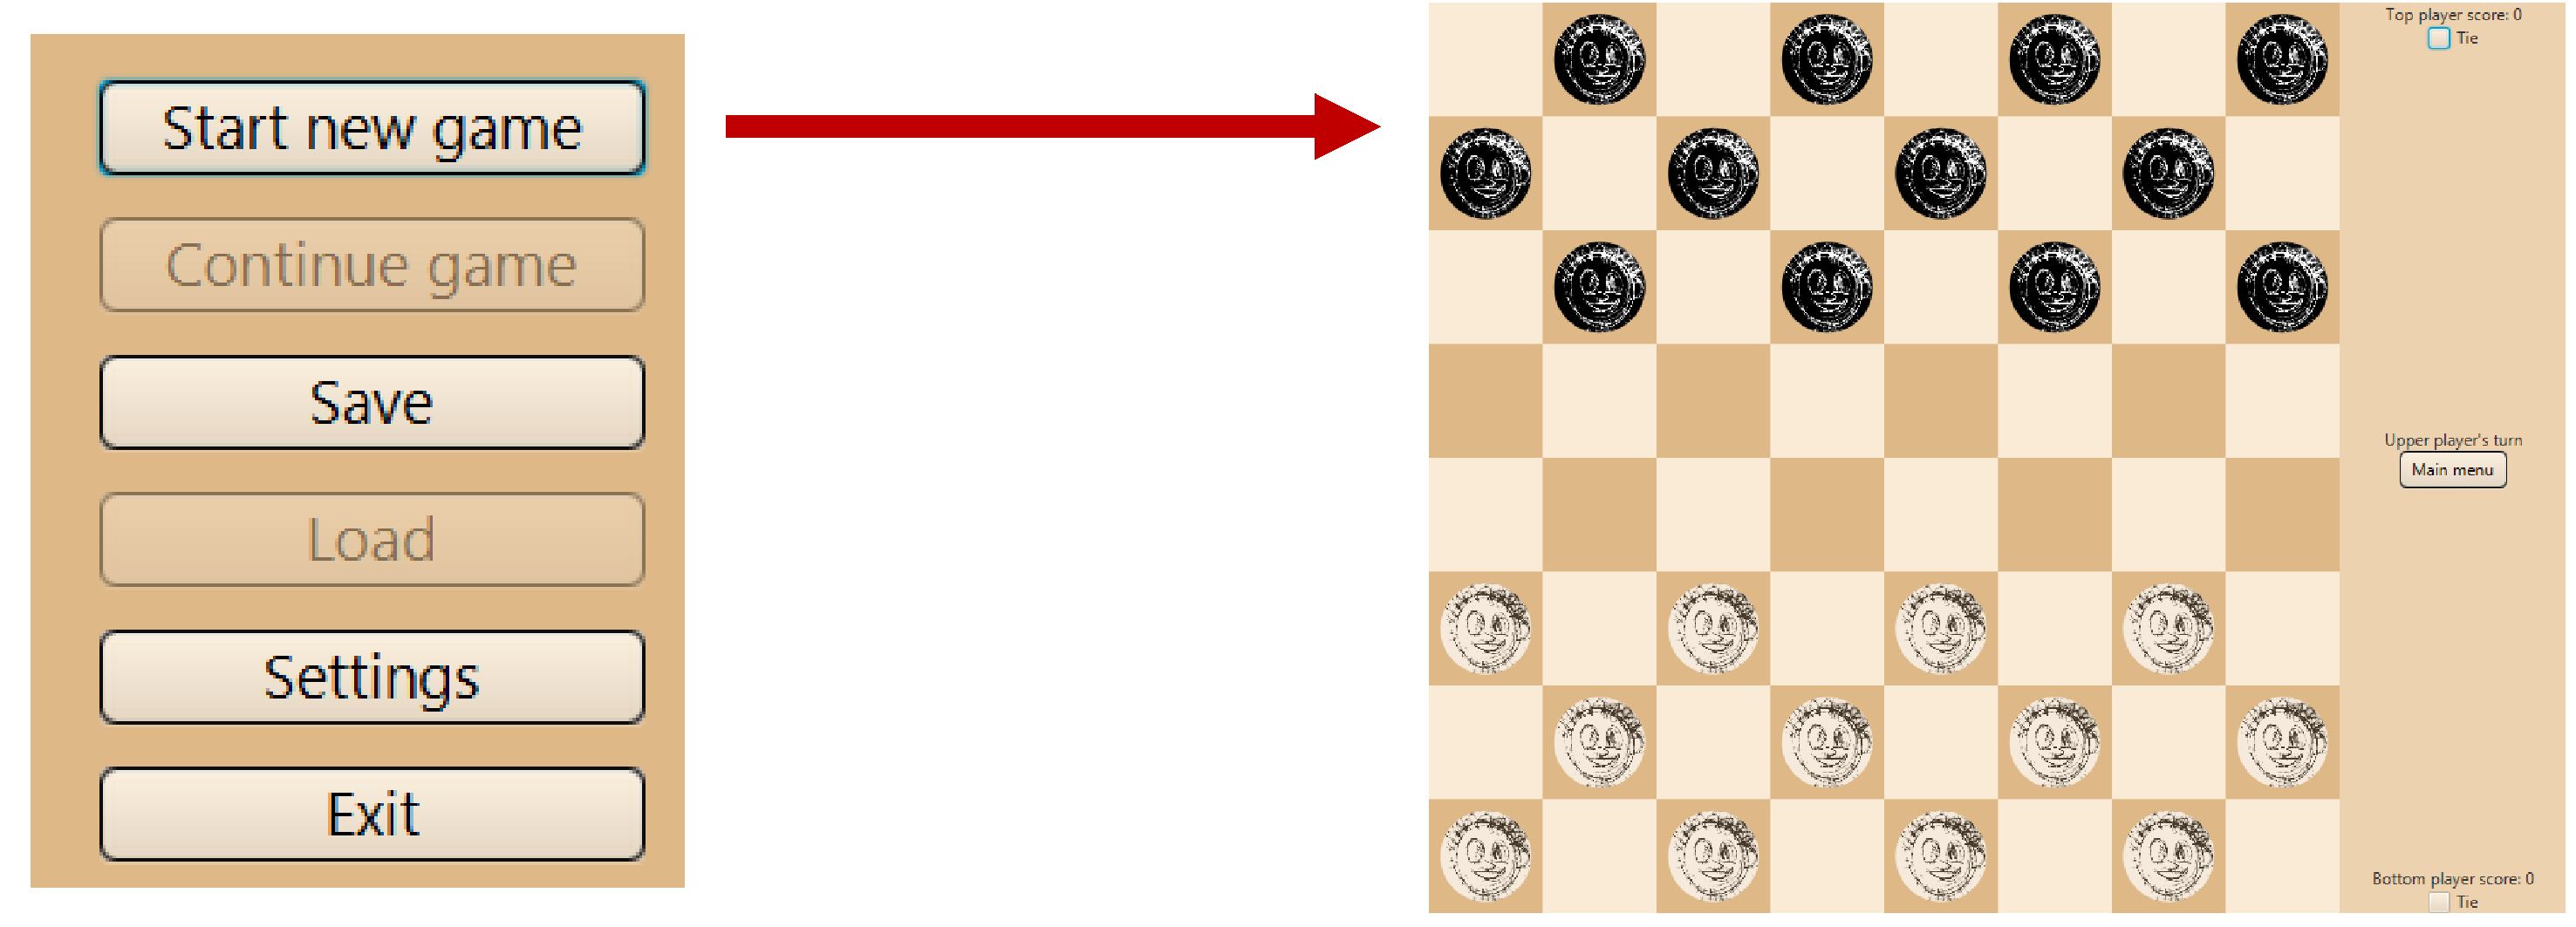
\includegraphics[width = 0.7  \textwidth]{Figurer/gameStart}
        \caption{Overgang fra main menu scenen til spil scenen når spillet startes. Her med standard størrelse 8x8.}
        \label{fig:gameStart}
    \end{figure}

% Magnus
% Hvordan ved jeg, hvis tur det er?
\textbf{Tur:} Spilleren får vink om, hvorvidt det er deres tur. I \textsc{SimpDam} kan du kun trække i dine brikker, når det er din tur. I \textsc{AvaDam} benyttes en del visuelle vink; Modstanderens brikker bliver lidt gennemsigtige. Når du trækker en brik, farves legale felter, du kan flytte til. I panelet til højre står også, hvilken spiller der har tur. Når der spilles mod en AI, animeres AI'ens træk. Disse features uddybes senere. En variabel, der indeholder hvis tur det er, lagres i en klassen \texttt{Control}, i field af typen \texttt{Player} (\texttt{enum} med \texttt{mulighederne Upper, Lower, None}).\\

% Magnus
% Hvordan flytter jeg en brik?
\textbf{Flytning af brik:} Brikker flyttes ved at trække musen, dvs.: Klik ned på brikken du vil flytte, træk til slutfeltet, slip musen. Når brikken tages op, opdateres fields i \texttt{Control}, der benyttes i senere metoder. Når brikken trækkes, tegnes brikken kontinuerligt, dvs. brikken følger med musen. Når spilleren slipper brikken over et felt, køres metoder gennem i klasserne \texttt{TopLevelControl} og \texttt{Control}\footnote{I \textsc{AvaDam} tjekkes også om et felt er en legal midlertidig destination i en combo}. Disse metoder tjekker om trækket var legalt.
\\

%   RR
% \item Kan man ombestemme sig, når man flytter brik? (før flyt er sket) Hvordan? (begge)
\textbf{Fortrydelse af valgt brik:} 
Så snart en brik er sluppet vil den enten få den nye position hvis det er et legalt træk, ellers sat tilbage på den originale plads. Dette gør det meget nemt at fortryde et træk da man kan slippe den hvor som helst, så længe det ikke indgår i et legalt træk. Ved at trækket var illegalt er det stadig den samme spillers tur. På den måde bliver det meget intuitivt og nemt at vælge en anden brik / vælge et andet træk. \\

% Magnus
% Virker spillet med touch screen?
\textbf{Touch screen:} Spillet virker ikke med touch screen, da touch screen mussetræk (dragging) og \texttt{JavaFX} ikke samarbejder optimalt. Vores program er afhængigt af at mussetræk påbegyndes og afsluttes, da vi anvender \texttt{setOnMouseClicked}, \texttt{setOnMouseDragged} og \texttt{setOnMouseReleased} fra \texttt{JavaFX}. Med touch screen kan man med hurtige og samtidige mussetræk forvirre \texttt{JavaFX}: \texttt{MouseClicked} kan forekomme uden \texttt{MouseReleased}.\\

% Magnus
% Kan man bruge keyboard til at spille spillet?
\textbf{Keyboard:} Keyboardet kan bruges i begrænset omfang til spillet. Når brugeren er i spillet, fås main menuen frem ved at trykke escape. Når brugeren er i menuer, kan piletaster og space bruges til interaktion. \\

% Magnus
% Hvad er model og view koordinater?(originalt fra implementering)
\textbf{Model og view koordinater:} I modellen findes et array \texttt{Tile}$[\, \, \,][\, \, \,]$ \texttt{board}, der lagrer brættets felter. Indekserne i board i hhv. x- og y-retning kaldes model koordinater, dvs. feltet \texttt{board[0][7]} har model koordinaterne (0,7). Når feltet tegnes i scenen, sker det i stedet på dets view koordinater. View koordinaterne afhænger af variablene \texttt{sceneWidth} og \texttt{sceneHeight}, der sættes i \texttt{View}, når programmet åbnes. De afhænger af skærmens størrelse:
\begin{lstlisting}
static double boardHeight = (Screen.getPrimary().getBounds().getHeight() - 100);
\end{lstlisting}
dvs. alle shapes, der tegnes, er skaleret i forhold til skærmens størrelse. Det gør spillet uafhængigt af skærmens opløsning, og således spilbart på de fleste skærme.\\

 \begin{figure}[H]
        \centering
        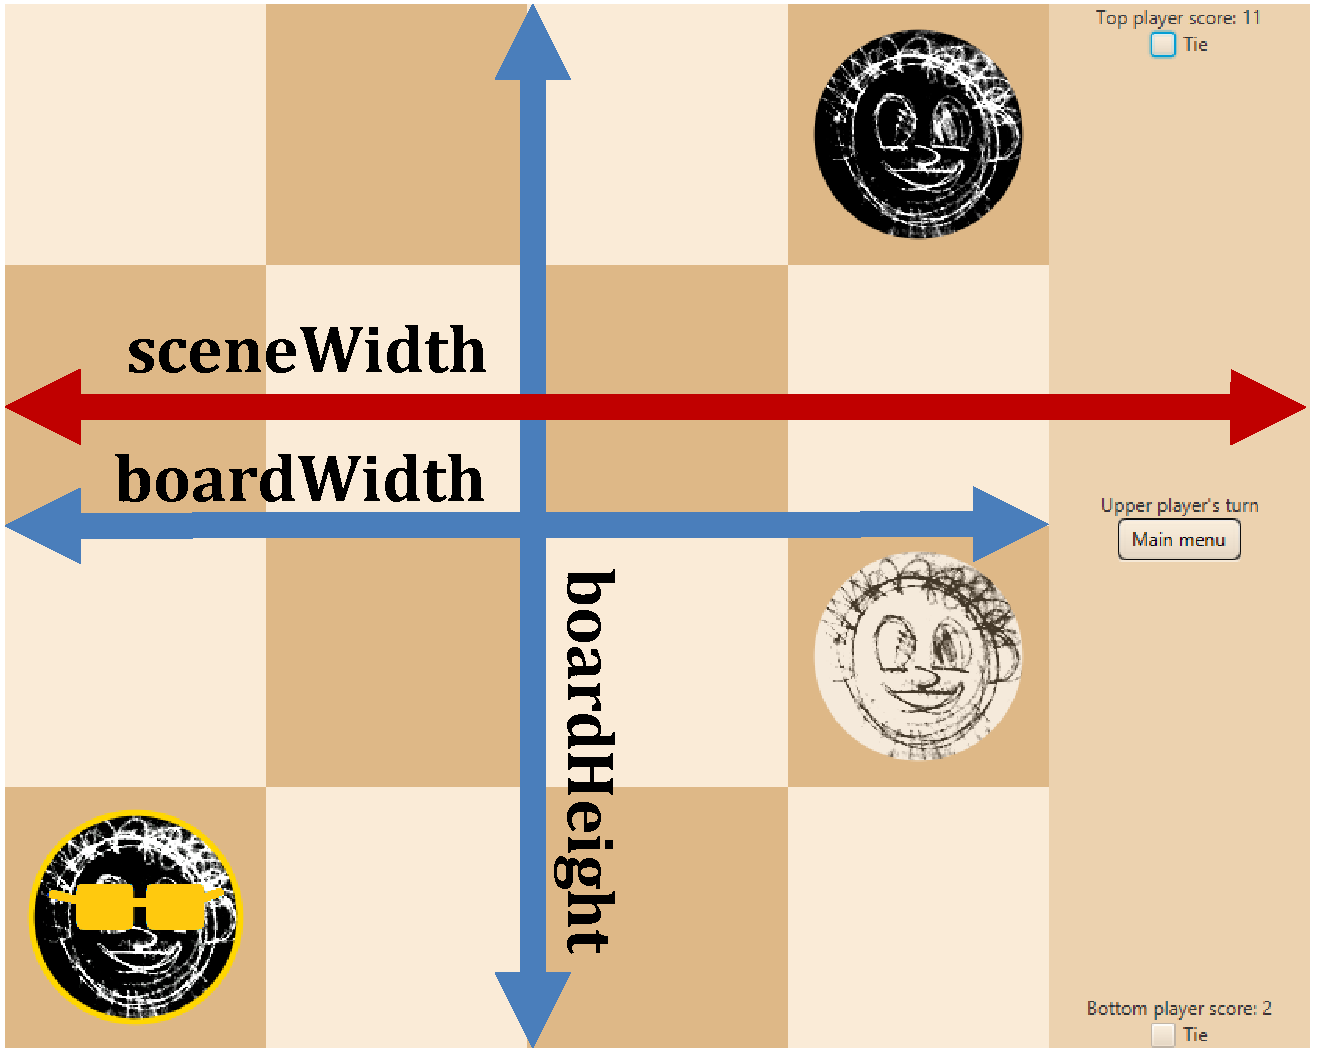
\includegraphics[width = 0.6  \textwidth]{Figurer/heightWidth.pdf}
        \caption{Visuel oversigt over størrelserne af \texttt{boardWidth}, \texttt{boardHeight} og \texttt{sceneWidth}.}
        \label{fig:heightWidth}
    \end{figure}

% Magnus
% Hvilke classes bruger spillet?
\textbf{Klasser:} Programmet bruger 15 klasser, fordelt i 3 kategorier: model, view og control. Klasserne gennemgås i detaljer i kategoriernes respektive afsnit, men i korte træk bruges klasserne i figur \ref{fig:MVC}. Ethvert felt på brættet er af typen \texttt{Tile}. Enhver brik er af typen \texttt{Piece}.

\subsection{\textsc{SimpDam}}\label{sec:designSimpDam}

%   RR
%    \item Hvordan må brikker flytte?

\textbf{Flytning af brikker:} 
I \textsc{SimpDam} skal en brik kun være i stand til at rykke diagonalt, og flytte ét felt af gangen. Hvis brikken kan dræbe skal den lande på feltet direkte efter fjenden og fjenden fjernes. En brik kan flytte som en kronet brik, både op og ned af brættet (stadig diagonalt). 
\\

%   RR
%    \item Hvordan ved jeg, hvilke legale træk en brik har?
\textbf{Visuelle indikationer:} 
\textsc{SimpDam} har ingen visuelle indikationer om legale træk. Brugeren flytter sin brik; hvis det går godt får brikken den nye position, hvis det går dårligt får brikken den gamle position. Spillet tager udgangspunkt i at spilleren kender til legale træk.
\\

%   RR
%    \item Hvordan ændrer jeg brætstørrelse? (terminal)
\textbf{Ændring af brætstørrelsen:} 
Hvis spillet køres ved at køre \texttt{.jar}-filen direkte vil man få standardstørrelsen på 8x8 felter. Hvis man vælger at køre filen gennem terminalen via \texttt{"java -jar SimpDam.jar"} vil man blive spurgt om at indtaste et tal mellem 3 og 100 hvor man derigennem vælger størrelsen af brættet. I tilfældet af illegalt input vil man få en fejlbesked og spillet startes med standardstørrelsen. 
\subsection{\textsc{AvaDam}} \label{sec:designAvaDam}
%Jens
%Er der instruktioner i hvordan spillet spilles?
\textbf{Brugervejledning:} \textsc{AvaDam} har ingen direkte brugervejledning i hvordan dam spillet spilles. Det antages at brugeren er kendt med dam, og specifikt danskdam.dk's regelsæt\footnote{Dansk Dam Forenings officielle hjemmeside: \url{http://www.danskdam.dk/}}, da det er dette spillet håndhæver. I alle tilfælde er spillets gang præsenteret på en intuitiv måde (fx via visuelle vink) så en uvidendende bruger højst sandsynligt hurtigt lærer de basale regler af spillet, blot ved at spille. \\

%Jens
%Hvilke regelsæt benyttes?
\textbf{Regelsæt:} \textsc{AvaDam}s regler tager udgangspunkt i det regelsæt der er redegjort af Dansk Dam Forening. Den eneste undtagelse af dette er hvorvidt en combo \textit{skal} fuldføres eller kan stoppes undervejs. Her er Dansk Dam Forenings regelbeskrivelse tvetydige og reglen er derfor blevet indført som en valgfri mulighed i spilindstillingerne.  \\

% Magnus
% Hvordan ved spilleren inde i spillet, hvilke regler der er på?
\textbf{Aktiverede regler:} Der er mange mulige regler i dam. De grundlæggende regler er altid aktive; Hvert felt kan kun have én brik stående. Brikker kan kun flytte diagonalt. Spilleren kan ikke slå sine egne brikker ihjel. \textsc{AvaDam} har dog yderligere regler, der kan aktiveres gennem menuen i checkbokse. De kan genkendes inde i spillet gennem visuelle vink. De aktivérbare regler er kort:

\begin{figure}[H]
    \centering
    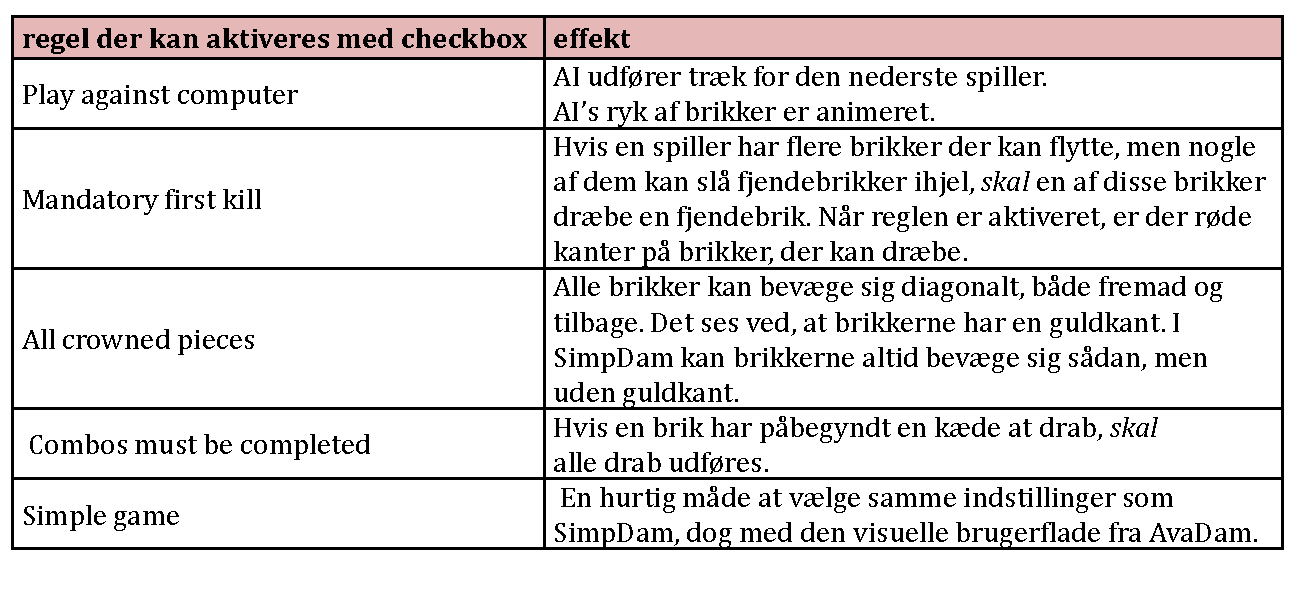
\includegraphics[width = 1.0 \textwidth]{Figurer/aktiveredeRegler.pdf}
    \caption{Aktivérbare regler i det \textsc{AvaDam}, og deres tilhørende effekt på spillet.}
    \label{fig:aktiveredeRegler}
\end{figure}

% Magnus
% Hvad betyder pointene?

\textbf{Score:} I \textsc{AvaDam} får hver spiller point for at flytte en brik (+1 point), og yderligere 9 point for at slå en fjendebrik ihjel. Pointene lagres i modellen \texttt{DamModel} i static fields. Scorene vises i panelet til højre for brættet.\\

%Jens 
%Nedenstående fire spørgsmål er placeret under samme kategori: visuelle indikatorer
%\item Hvordan ved jeg, hvilke legale træk en brik har?
%\item Hvad er forskellen på grøn og gult highlight?
%\item Hvad betyder kantfarverne? rød + gul.
%\item Hvordan genkender jeg en kronet brik?

\textbf{Visuelle indikatorer:} For at holde brugeren opdateret på spillets gang og for at håndhæve spillets regler, er der designet tre typer visuelle indikatorer; farvede kanter på brikker, farve fremhævning af felter og gennemsigtighed af brikker. 
\begin{enumerate}
    \item For at klargøre hvilken spillers tur det er bliver den ikke-aktive spillers brikker gjort 30\% mere gennemsigtige.
    
    \item For at vise særligt gældende regler/egenskaber for bestemte brikker, farveslægges disse brikkers kanter. En kronet brik, får en gyldengul kant når de bliver kronet. Hvis indstillingen \texttt{"Mandatory first kill"} er valgt, får aktive-spillers brikker, som kan udføre et drab, ændret kantfarve til rød. Hvis en brik har rød kant, er det den eneste brik der kan rykkes. Hvis flere brikker har rød kant vælges frit mellem disse. Indikationerne ses bl.a. på forsidens figur. 
    
    \item For at vise hvilke legale træk der kan tages med en valgt brik, bliver samtlige mulige legale felter fremhævet med én af to farver. Felter fremhævet med lysegrøn repræsenterer mulige felter hvor trækket kan afsluttes, se figur \ref{fig:MovePieceFigure}. \begin{figure}[H]
        \centering
        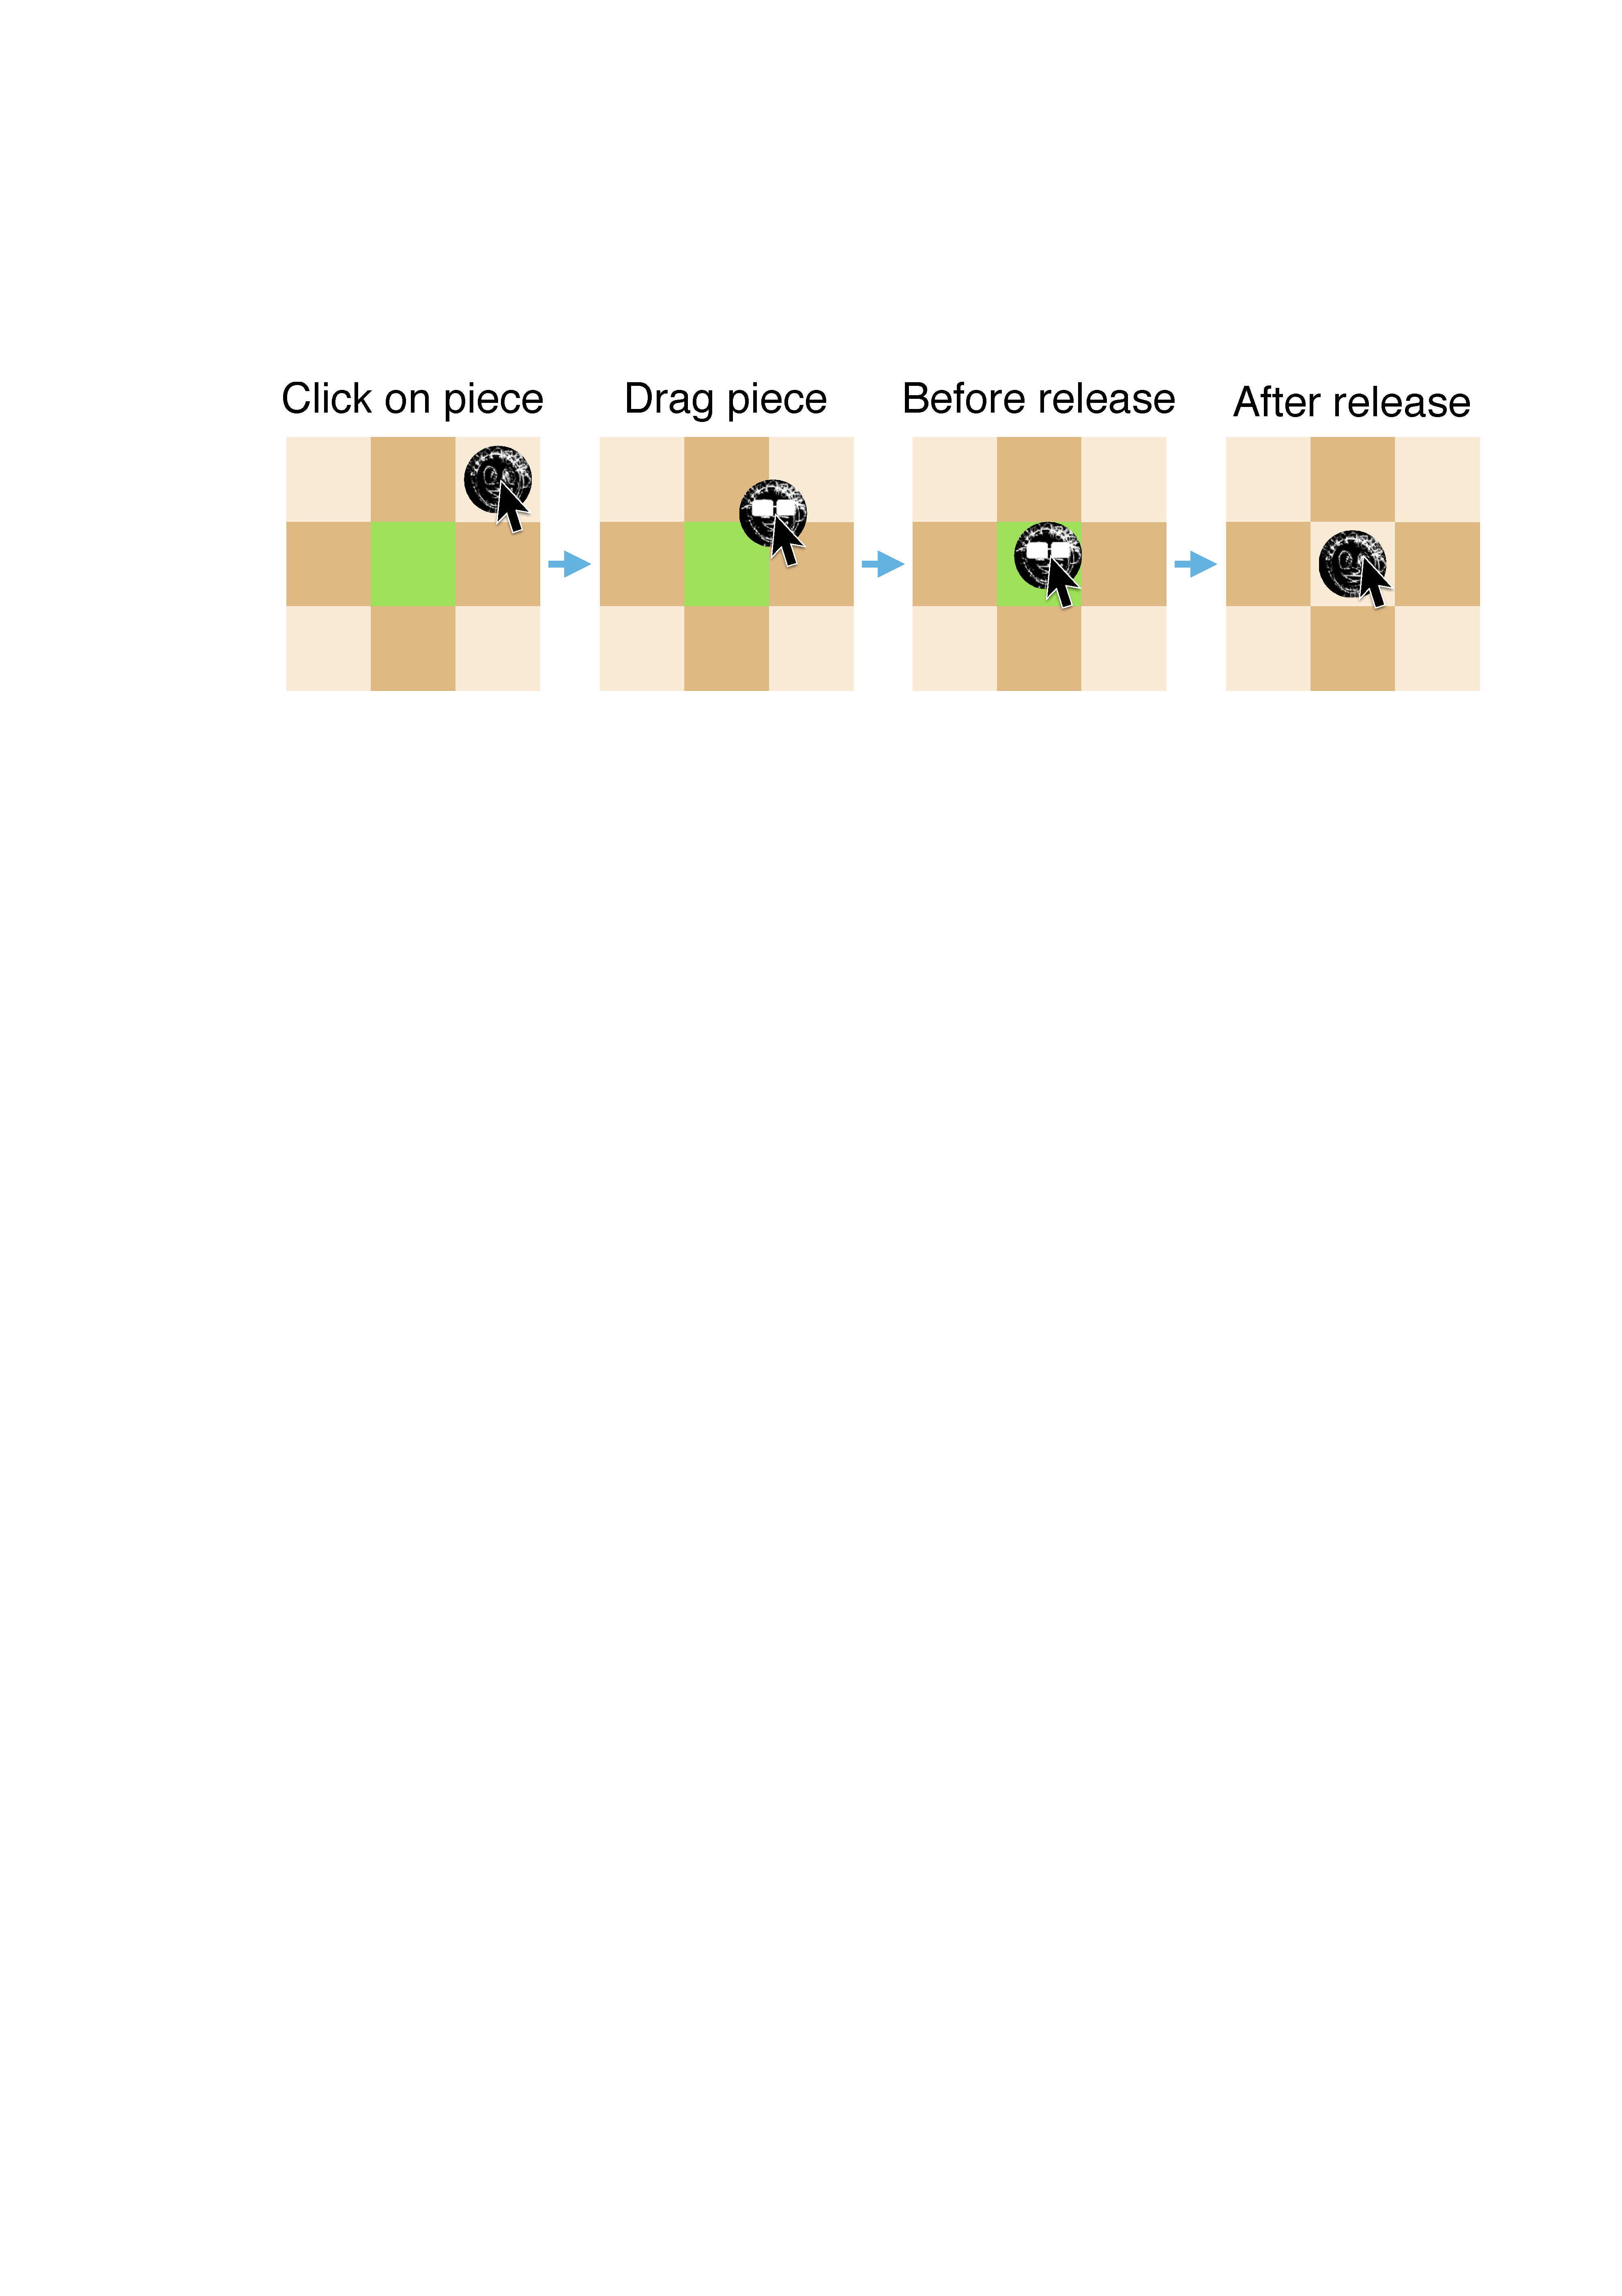
\includegraphics[width = \textwidth]{Figurer/MovePieceFigure}
        \caption{Illustration over hvordan legale felter fremhæves med lysegrøn farve når en brik vælges.}
        \label{fig:MovePieceFigure}
    \end{figure}

    Hvis trækket involvere et drab, vil et grønt felt skifte farve til gyldengul, når den markeres over. Dette indikere at en combo er påbegyndt. Hvis det ud fra det nyligt markeret gule felt er muligt at lave endnu et drab med samme brik, vil dette korresponderende felt nu lyse op med grønt - og således foreslå et nyt legalt afslutningsfelt. Spilleren kan nu vælge at fortsætte sin combo eller at afslutte den på det gule felt ved at slippe musemarkøren\footnote{I spilindstillingerne kan færdiggørelsen af en combo gøres obligatorisk}. Spilleren fortætter comboen ved at markere det nye grønne felt og dermed gøre det gult. Til slut, før musemarkøren slippes, viser de gule felter den rute som brikken "bevæger" sig over i løbet af trækket. Se nedenstående figur \ref{fig:ComboFigure}.
     \begin{figure}[H]
        \centering
        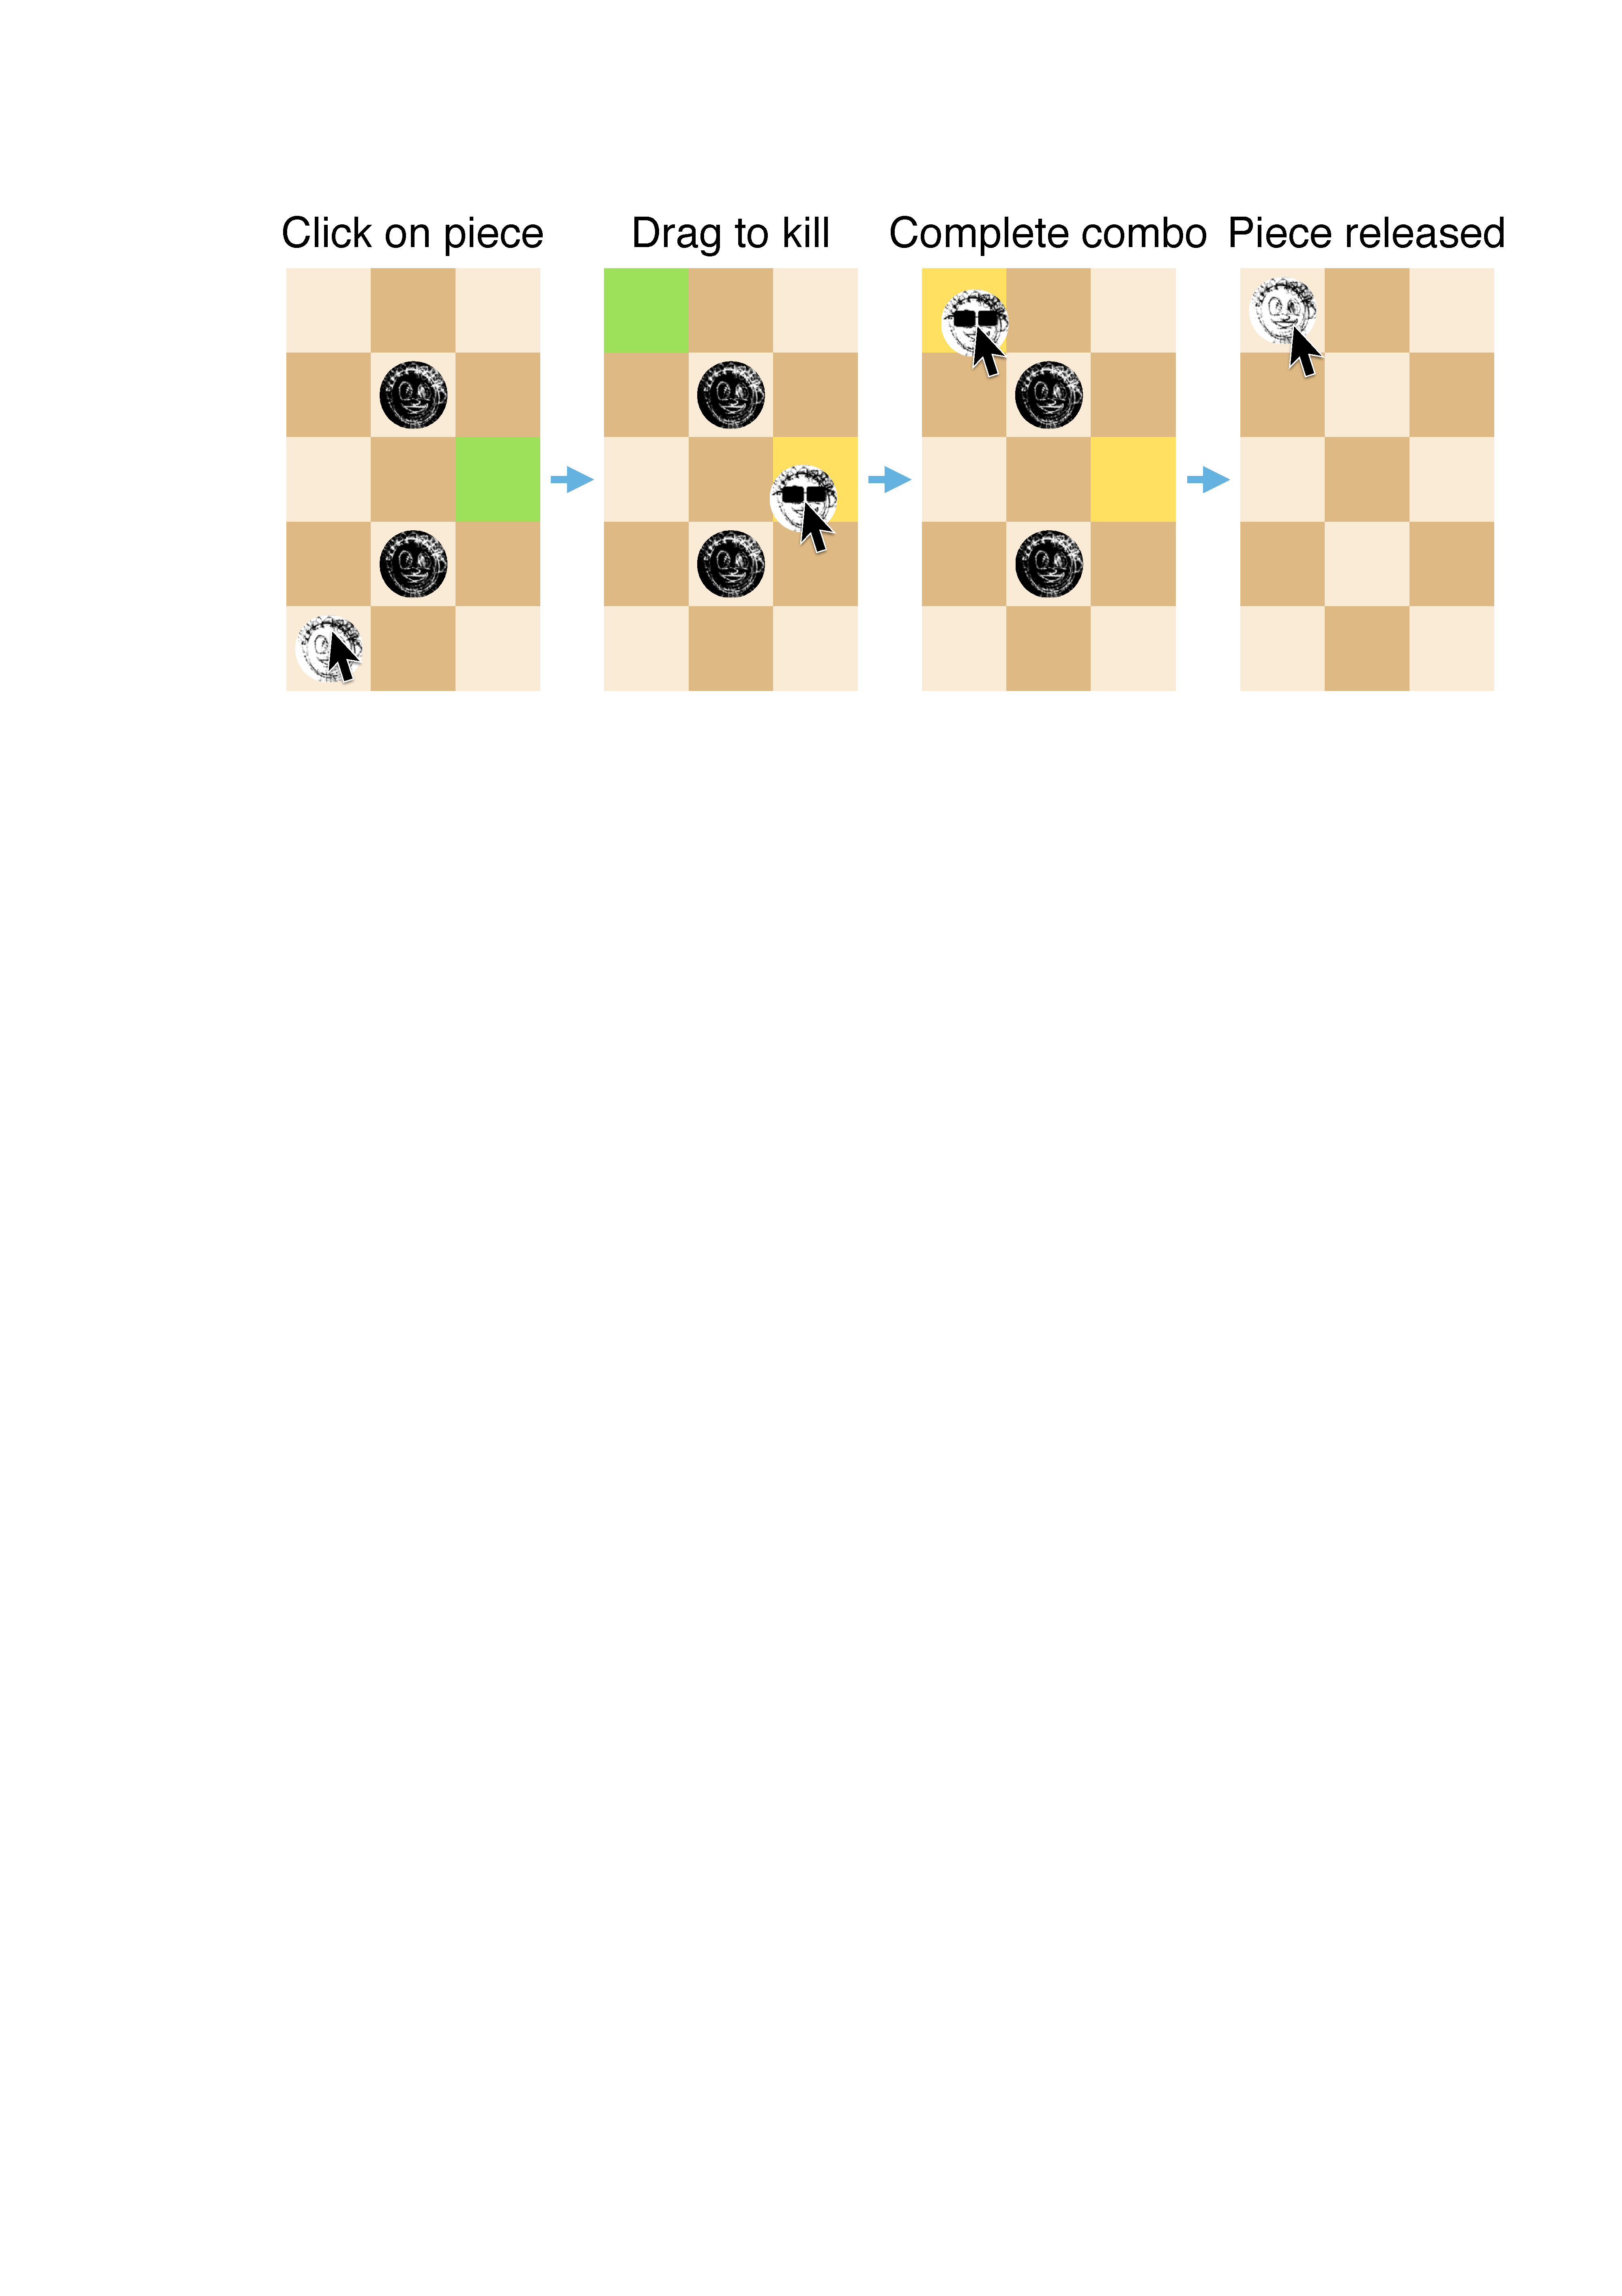
\includegraphics[width = \textwidth]{Figurer/ComboFigure}
        \caption{Figur over hvordan udførelsen af en combo bliver indikeret og udført.}
        \label{fig:ComboFigure}
    \end{figure}
\end{enumerate}
  
%Jens
%Hvordan ændrer jeg brætstørrelse? (slider)
\textbf{Brætstørrelse:} Inde i spilindstillingerne findes en slider som kan justere størrelsen af brættet. Denne effekt træder først i kraft når en nyt spil startes.\\

% Magnus
% Hvordan skalerer spillet på større/mindre skærme? (begge)
% Er resizing muligt undervejs? (advdam)
\textbf{Skalering på skærme og resizing:} Da størrelsen af vores tegnede shapes er baseret på view koordinater, der skaleres efter scenens størrelse, skaleres spilvinduet efter programbrugerens skærmstørrelse (eller egt. opløsning). Til forskel fra \textsc{SimpDam}, er der i \textsc{AvaDam} forskel på scenens vidde og højde; panelet med score og uafgjort knapper til højre er dog også skaleret efter skærmens højde. Det er ikke muligt at ændre vinduets størrelse ved at trække i vinduets hjørne. \\

%   RR
%   \item Hvad er gjort for at gøre spillet underholdende? (advdam)
\textbf{Underholdning i spillet:} 
For at bringe yderligere underholdning ind i spillet er der tilføjet at brugeren kan skifte billeder (samt gifs) for hvert holds brikker. Eksempler på disse billeder ses i figur \ref{fig:ShowcasePieces}. Vi har også introduceret forskellige spilleregler for at indføre variation.
\\
\begin{figure}[H]
    \centering
    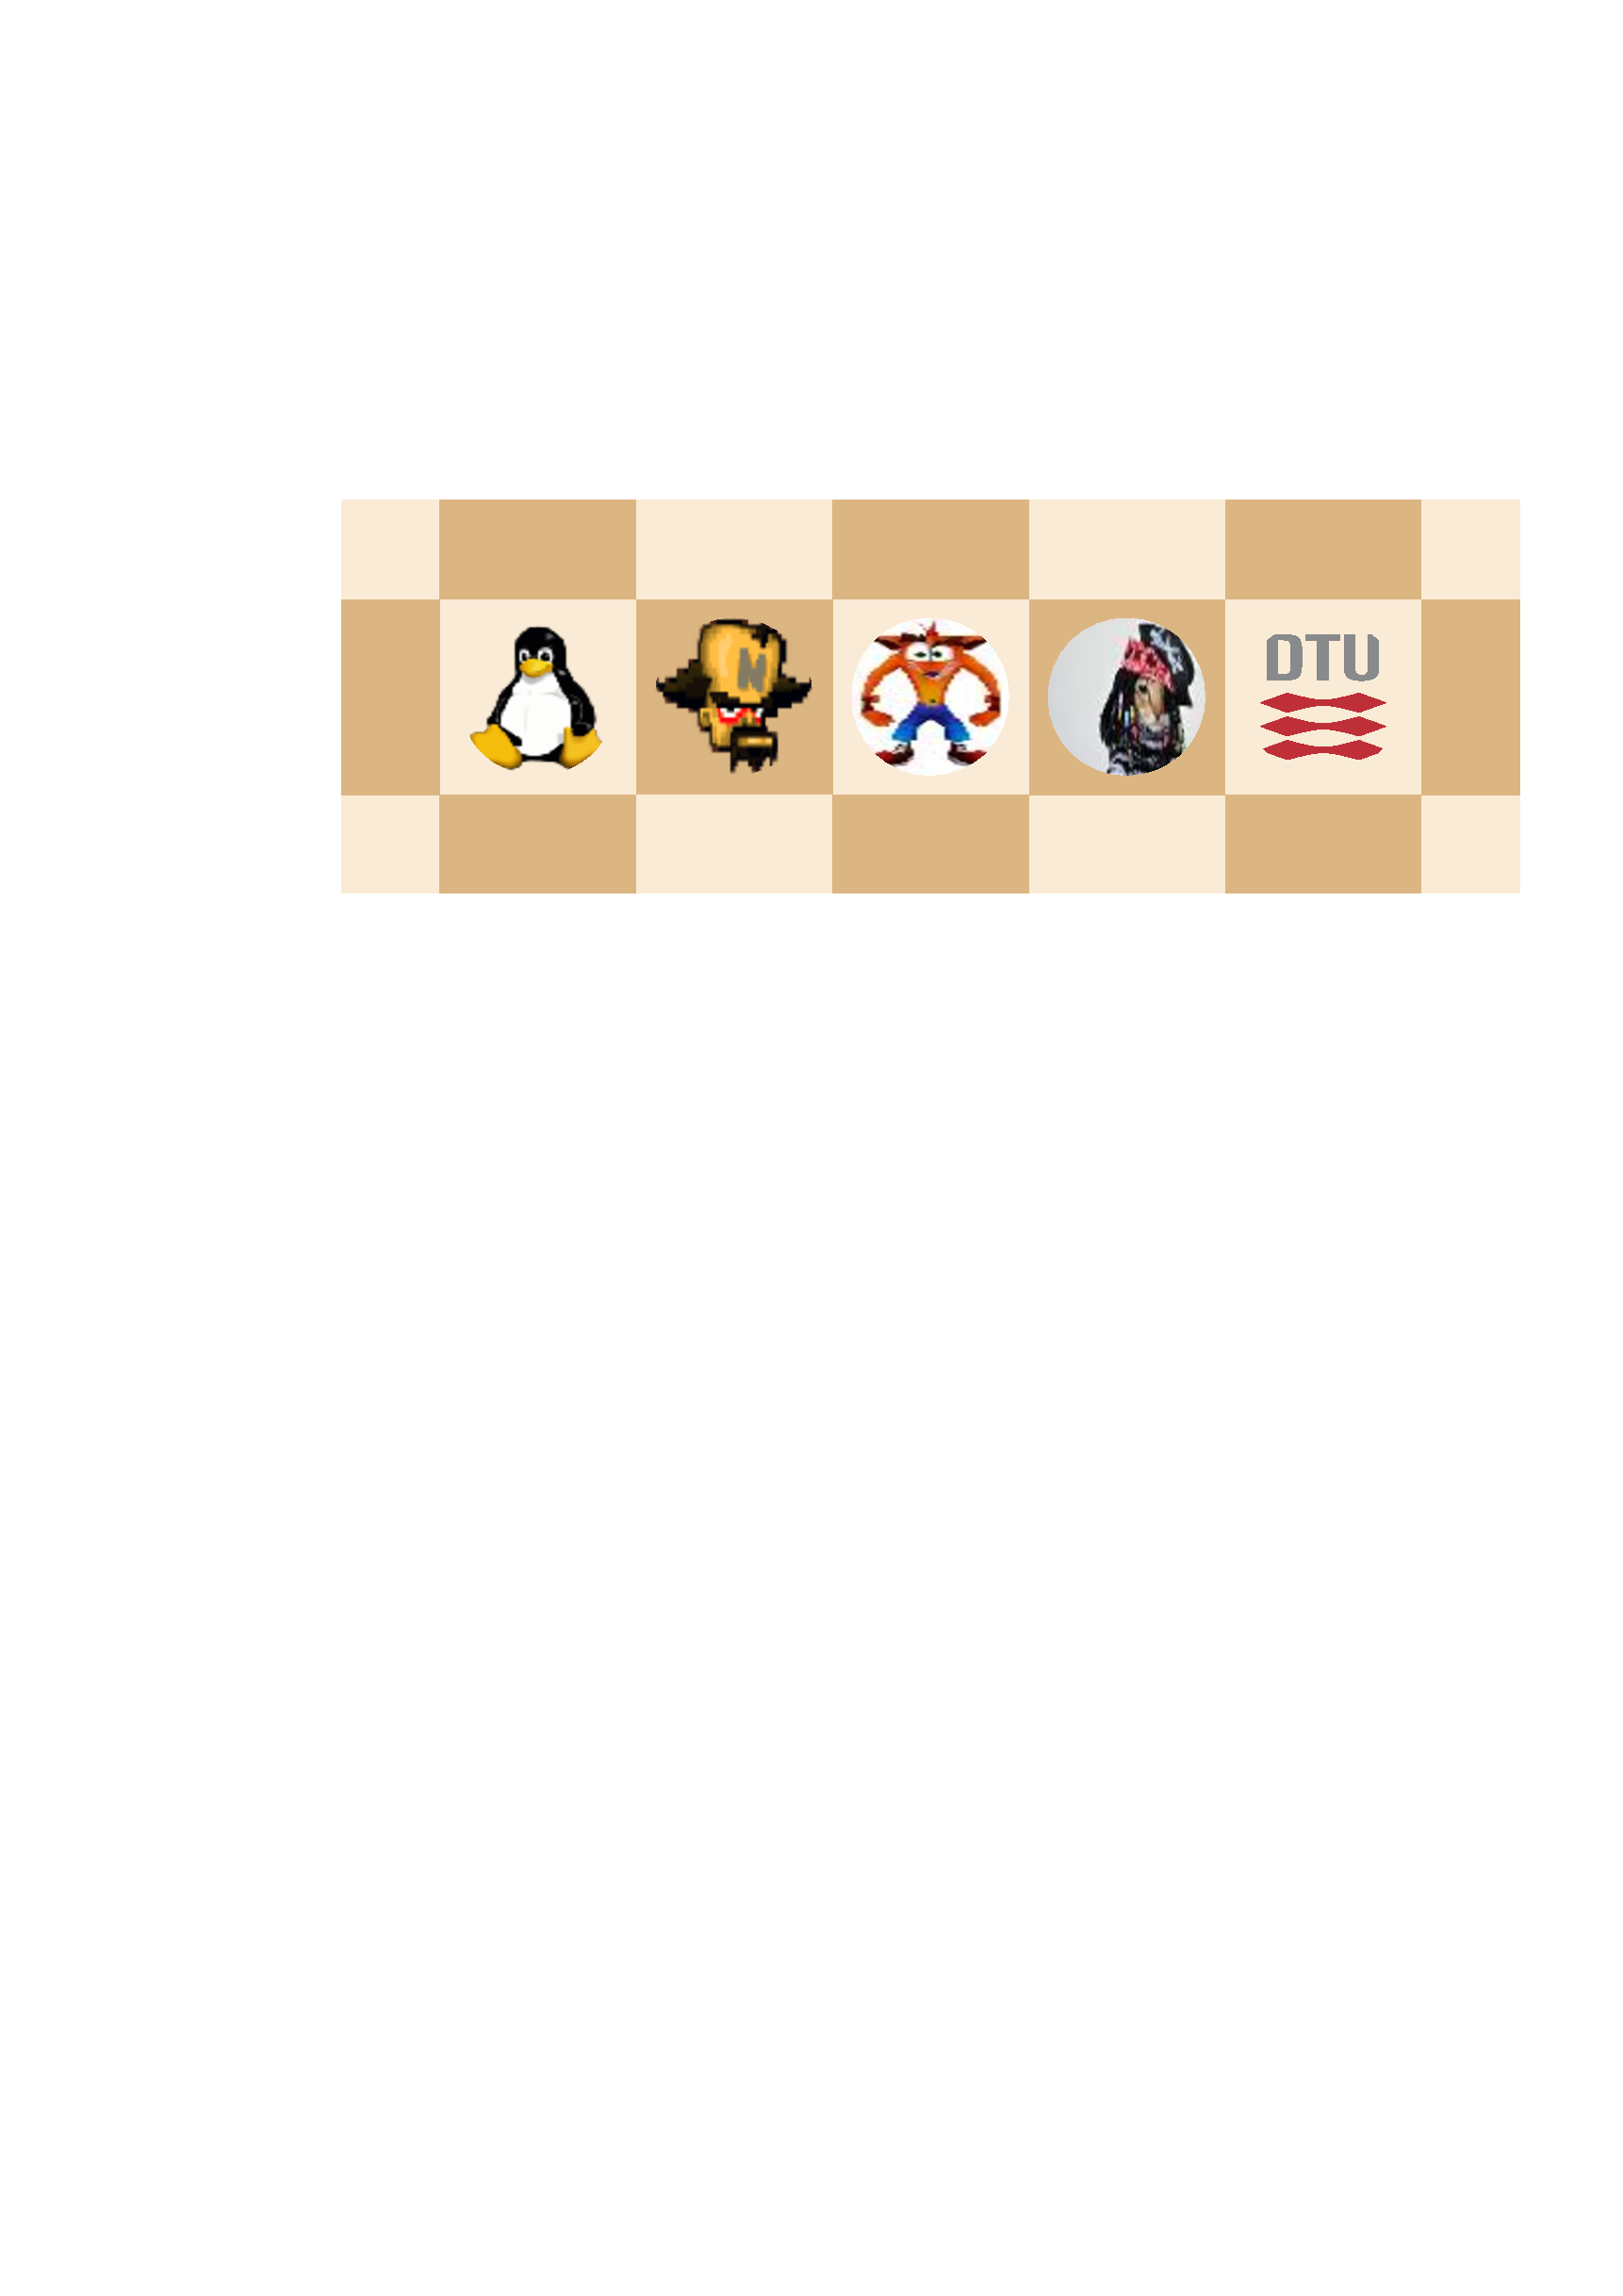
\includegraphics[width = 0.9 \textwidth]{Figurer/ShowcasePieces.pdf}
    \caption{Eksempler på billeder, spilleren kan uploade til sine brikker. Når spilleren vælger et billede, vil det bliver vist på alle spilleren brikker. Billedtyper understøttet: \texttt{.png, .jpeg, .gif, .jpg,  .bmp}.}
    \label{fig:ShowcasePieces}
    \end{figure}

%Jens
%Hvilke typer billeder kan jeg uploade? (gif, transparent)
\textbf{Tilpasselige brik-billeder:} Det er i spilindstillings menuen muligt at ændre på billederne brugt til begge holds brikker. Knapperne under \texttt{"Choose custom images"} åbner en \texttt{FileChooser} hvis tilladte extensions er: \texttt{ .png, .jpeg, .gif, .jpg,  .bmp}. Det valgte billede bliver gemt som et nyt objekt af typen \texttt{Image}. Herfra bliver billedet brugt til at danne et nyt objekt af typen \texttt{ImagePattern}. Dette format kan anvendes som et \texttt{Fill} i et \texttt{JavaFX Shape}. Det nye billede træder i kraft, når brugeren starter et nyt spil.\\

% Magnus
% Hvordan markeres kongebrikker? Billeder på billeder, eller udskift? (advdam)
\textbf{Kronet brik billede:} Hvis brugeren beholder standardbillederne på sine brikker, markeres kronede brikker yderligere ved udskiftning af billedet. Dette ses i figur \ref{fig:defaultPieces}. Den kronede brik har et guldbriller på! Dette er opnået ved at udskifte billedet på brikken, så hvis der uploades selvvalgte billeder, tilføjes der kun guldkant på brikken.  \\

\begin{figure}[H]
    \centering
    \includegraphics[width = 1.0\textwidth]{Figurer/DefaultPieces}
    \caption{Oversigt over standardbrikkerne for de to hold. Fra venstre til højre er det: Standard, valgt, kronet, kan dræbe og ikke valgbar.}
    \label{fig:defaultPieces}
    \end{figure}

%R  R
%   \item Hvad er gjort for at gøre spillet rart i gameplay? (advdam)
\textbf{Tilfredstillelse i spillet:} 
For at gøre spillet mere tilfredsstillende at spille er der tilføjet at brikker følger musen mens man flytter den, for at gøre hele oplevelsen mere virkelighedstro. Når man placerer en brik snapper den automatisk til feltets centrum.
\\

%   RR
%   \item Hvordan animeres spawn og død? 
\textbf{Animationer for spawn og død:} 
En brik spawnes ved at skaleres fra en prik med radius 0 til dens egentlige størrelse. Dette sker hver gang man går ind i spillet, uanset om det er et nyt spil eller et fortsat spil. En brik dræbes/fjernes ved at skaleres dem ned fra dens egentlige størrelse til en prik med radius 0. Dette sker hver gang en brik bliver dræbt. Målet med animationerne er at give en mere flydende overgang for spilleren. Pludselige ryk i brikker kan virke fejlfyldt og derfor uønsket.\\


% Magnus
% Hvad er begrænsningerne for spillet? (RAM) (advdam)
\textbf{Ressourcebegrænsninger for spillet:} Spillet virker ikke overvældende ressourcekrævende. Selv når spillet kører 50 gange 50 felter, og vi uploader gifs til brikkernes overflade, er det smooth. Ved 100 gange 100 felter med gifs er det ikke smooth, men spilbart. \\

%Jens
%Hvad gør continue knappen?
\textbf{Continue knappen:} Continue knappen skifter fra menuen tilbage til det spil der er i gang med at blive spillet.  \\

%   RR
%   \item Hvordan spiller jeg mod computeren?
\textbf{Spille mod AI:} 
Hvis man vil vælge at spille mod spillets AI gøres det gennem \texttt{"Settings"} menuen via checkboxen \texttt{"Play against computer"}.\\

%Jens
%Hvordan udløser jeg et uafgjort spil?
\textbf{Uafgjort spil:} Til højre i spil panelet findes to tie-checkboxes, én for hver spiller. Hvis begge er markeret afsluttes spillet og en besked i midten af brættet vises som fortæller at spillet er slut og endte uafgjort. \\
%   RR

%   \item Hvordan gemmer jeg og loader et spil?
\textbf{Loading af spil:}
Når spillet startes tjekkes om der findes en gyldig gemt fil. Hvis der findes en gyldig gemt fil vil \texttt{"Load"} knappen i main menu blive aktiv, hvis ikke vil den være inaktiv og først aktiveres igen når man gemmer spillet gennem \texttt{"Save"} knappen. Antaget at der findes en gyldig gemt fil og at man trykker på \texttt{"Load"} fra main menu, vil man blive dirigeret ind i spillet genereret fra den gemte fil. \\

% Magnus
% Er der lyde med? Hvorfor/hvorfor ikke?
\textbf{Lyde:} Vi eksperimenterede med lyde i tidligere versioner af programmet (baggrundsmusik, lyde ved drab), men det blev senere nedprioriteret. Vi har dog fået et indblik i, hvordan lyde kan tilknyttes events.

\section{Implementering}
\subsection{Overordnet}\label{sec:ImpOverordnet}

% RR
%   \item Hvilken platform har I brugt til view? (Swing, JavaFX) 
\textbf{GUI platform:} 
Spillet er lavet ved brug af \texttt{JavaFX} frem for \texttt{Java Swing}. Dette var en beslutning helt fra starten, da \texttt{JavaFX} forventes at erstatte \texttt{Swing} og at \texttt{JavaFX} har nemmere tilgang til event listeners. \\

% RR
%   \item Hvorfor bruger I JavaFX shapes i modellen? 
\textbf{JavaFX Shapes:} 
Klasserne \texttt{Piece} og \texttt{Tile} nedarver hhv. \texttt{Ellipse} og \texttt{Rectangle} fra \texttt{JavaFX Shapes}. Dermed har alle brikker og felter nem adgang til bruger input gennem event listeners. Eventuelle egenskaber som \texttt{Fill} og \texttt{Stroke} kan også bruges uden yderligere implementation. 
\\

% RR
%    \item Hvordan håndteres FPS?
\textbf{FPS (Frames Per Second): } 
Spillet opdaterer kun modellen, når der er bruger-input. GUI'en udnytter \texttt{JavaFX}'s Application til at styre opdatering af billedet. Ved ikke at opdatere modellen 30-60 gange i sekundet bliver hele spillet mindre ressourcekrævende. I stedet bliver metoder kaldt af listeners fra de implementerede \texttt{JavaFX Nodes} og \texttt{Shapes}. \\

% RR
%    \item Hvor mange ressourcer kræver spillet?
\textbf{Computer ressourcer:} 
Som tidligere nævnt er opdateringen af modellen kun igangsat når nødvendigt, hvilket sparer mange ressourcer. Dog skal hele brættet og alle brikker initialiseres når spillet starter. Dermed er spillets ressourceforbrug klart størst når et nyt spil startes, hvorefter det bruger størstedelen af tiden i en tilstand med lavt ressourceforbrug. 
\\

% \item \item Hvorfor er alt static?
\textbf{Static:} 
Vi har valgt at bruge static fields og metoder, eftersom vi ikke initialiserer fx \texttt{Control} og \texttt{TopLevelControl} klasserne. Med denne brug af static bliver tilgangen til kontrol betydeligt simplere. Det gør dog grupperne af klasser i model-view-control designmønstret mindre uafhængige.
\\

% RR
%Hvordan håndteres abstraktionsniveau i kontrollen?
%   &
%Hvad er TopLevelControl?
\textbf{Abstraktionsniveauer i Kontrollen:} 
Programmets kontrol er delt op i to klasser: \texttt{Control} og \texttt{TopLevelControl}. Klassen \texttt{Control} indeholder metoder der kigger direkte på brættet og brikkernes positioner. For at bruge \texttt{Control} mest hensigtmæssigt, blev TopLevelControl indført som mellemmand. I \texttt{TopLevelControl} findes metoder kaldes på særlige tidspunkter i løbet af en spillers tur. Ved at have denne opdeling, kan brikkerne bruge de højere abstraktionsniveauer i kontrollen uden at tage sig af hvad der sker mellem \texttt{TopLevelControl} og \texttt{Control}. 
\\

% RR
%    \item Hvordan bruges model og view koordinater? 
\textbf{Model og view koordinater:} 
I spillet bruges 2 sæt koordinater: \textit{Model} koordinater og \textit{View} koordinater. Model og view koordinater er til for at styre brikkernes aktuelle placering på skærmen (view koordinater) og brikkernes (samt felternes) placering på brættet (model koordinater). Oversættelsen fra det ene koordinatsæt til det andet bruger metoderne \texttt{toModelCoord} og \texttt{toViewCoord}: 

\begin{lstlisting}
static double toViewCoord(int i) {
	return i * tileSize + tileSize / 2; }

static int toModelCoord(double d) {
	return (int) (d / tileSize); }
\end{lstlisting}

Ved at bruge model koordinater undgås meget forvirring og datamanipulation i kontrollen. Hoveddelen af spillets logik foregår i model koordinater, som oversættes til view koordinator når brikker skal flyttes. Disse to sæt af koordinater bidrager til adskillelse mellem Model og View, i MVC designmønstret. \\


% RR
%    \item Hvordan navngiver I methods og variable?
\textbf{Navngivning af fields og metoder:} 
Vi har stilet efter bruge forklarende navne til variable. Dette har været et udfordrende element når vi løbene har redigeret kode i løbet af projektet \footnote{Eksempelvis har mange metoder fået tilføjet funktionalitet undervejs i projektet. Så skulle metodens navn opdateres!}. Hvis en metode returnerer en boolean har vi så vidt muligt også gjort metodenavnet til en udsagn som den returnerede booleanværdi svarer på om er sand eller falsk. Hvis metoder har større funktionalitet (hvis det fx er en \textit{mutator}) er et passende navn fundet med en mere dybdegående forklaring i dens deskription. \\

% RR
%Hvordan ved læseren af koden, hvordan en method virker/bruges? (comments)
\textbf{Metode deskriptioner:} 
Hver metode har en deskription som gør at man udefra nemt kan se hvad metoden gør samt hvilke parametre den forventer og hvilken returværdi den tilbageleverer. Et eksempel er givet ved:

\begin{lstlisting}
/**
* Chooses a piece for the AI to move.
*/
\end{lstlisting}

%   RR
%   \item Hvor ens er SimpDam og AvanceretDam? 
\textbf{Forskel på \textsc{SimpDam} og \textsc{AvaDam}:} 
\textsc{SimpDam} var en af de tidligere versioner af spillet. \texttt{Control} klassen i \texttt{SimpDam} tager udgangspunkt i en anden fremgangsmåde end \texttt{Control} i \textsc{AvaDam}. Når en brik slippes i \textsc{SimpDam}, tjekkes om det var et legalt træk. I \textsc{AvaDam} tjekkes først alle legale træk. Når en brik slippes, tjekkes om det var én af de fundne (legale) pladser. Metoden i \textsc{SimpDam} lægger ikke op til indføre comboer. Så vi har fulgt en anden tilgang i \textsc{AvaDam}. Andre forskelle er mere åbenlyse: \textsc{AvaDam} har  menuer, visuelle indikationer, indstillinger og et sidepanel.\\

% RR
%Hvordan afholder I den "forkerte" spiller fra at trække, når det ikke er deres tur?
%   &
% Hvordan styres, hvis tur det er? 
\textbf{Spillerens tur:} 
I klassen \texttt{Control} findes et field som indeholder hvem den nuværende spiller er. Dette er implementeret ved at bruge en enumeration placeret i brikken selv: 

\begin{lstlisting}
enum Player {
	Upper, Lower, None; }
\end{lstlisting}

Derved kan der kun ske interaktion, hvis brikken der skal flyttes har samme værdi som fieldet \texttt{currentPlayer} i klassen \texttt{Control}. Dette field skifter værdi hver gang en tur afsluttes. Ved at have en spiller type \texttt{"None"} kan spillet gøres inaktivt og dermed gøre at brikker ikke kan flyttes hvis spillet er vundet, tabt eller uafgjort. Dette medfører også at der bliver brugt minimale ressourcer hvis en spiller prøver at tage fat i modstanderens brik. 
\\

% RR
%   \item Hvordan snappes brikker til tiles? (visuelt)
\textbf{Når brikker slippes:} 
Ved brug af model og view koordinater kan en brik nemt placeres i midten af det valgte felt. Dette håndhæves ved heltalsdivisionen i oversættelsen fra view til model og tilbage til view koordinater igen.  \texttt{toViewCoord} metoden forskyder samtidig positionen med halvdelen af størrelsen af felters længde, eftersom at brikker bliver placeret med hensyn til centrum. På den måde kan brikker også placeres nemt i felternes centrum uafhængig af brikkens radius.
\\

\subsection{\textsc{SimDam}}\label{sec:ImpSimp}
\subsubsection{View}
%% MIKKEL %%
% Hvad sker der når spillet startes
\textbf{Setup af spillet:} 
\texttt{View} klassen indeholder \texttt{main} metoden som iværksætter programmet, så programmet starter fra \texttt{View}. I \texttt{View} bliver metoden start kørt, der sætter en \texttt{Stage} op. Der skabes et \texttt{Layout root} i form af et \texttt{BorderPane}, og en \texttt{Scene}. \texttt{DamModel} instantieres, og tilføjes til \texttt{root}. Størrelsen af \texttt{stage} sættes efter \texttt{root}, og \texttt{stage} vises. Højden og bredden af \texttt{root} sættes ud fra højden af computerens skærm, så den automatisk tilpasses enhver computer. Højden og bredden kan sættes ud fra den samme parameter, da brættet er kvadratisk.\\ 

%% MIKKEL %%
% Hvordan håndteres user input?
\textbf{User input:} I \textsc{SimpDam}  håndteres bruger input på to forskellige måder. Først sætter brugeren et tal som parameter når spillet eksekveres gennem kommandoprompten. Hvis dette tal opfylder $n \in \{3, .., 100\}$, bliver det brugt til at sætte antallet af felter. \texttt{tileAmount} er antallet af felter der er i hver dimension af brættet. \texttt{tileAmount} bliver sendt videre til modellen. Størrelsen af felterne (\texttt{tileSize}) sættes ud fra \texttt{tileAmount} og bredden af scenen. 
Derefter opsættes GUI'en, hvorefter brugeren interagerer med spillet gennem denne GUI. Her kan man trække i pieces med musen, hvilket bliver håndteret med event listeners. Når en brik bliver flyttet, køres metoden \texttt{dragThisPiece} i klassen  \texttt{TopLevelControl}. Ved brug af \texttt{dragThisPiece} sættes brikkens position til musens position, såfremt musen er indenfor brættet. I x-retningen kontrolleres dette ved følgende stykke kode:

\begin{lstlisting}
if (mouse.getSceneX() > piece.getRadiusX()
	&& mouse.getSceneX() < View.tileAmount * tileSize - piece.getRadiusX()) {
	    piece.setCenterX(mouse.getSceneX());
}
\end{lstlisting}

I y-retningen sker det på en tilsvarende måde. \\
Når man slipper en brik, køres metoden \texttt{finishThisPiece} i \texttt{TopLevelControl}, der kører metoden \texttt{isLegalMove} i \texttt{Control}. \texttt{isLegalMove} checker, om brikken er sluppet over et legalt felt, og returnerer en boolean. Hvis det var et legalt træk, bliver det efterladte brik tildelt denne nuværende position. Hvis trækket er illegalt, bliver brikken sat tilbage til hvor den var før flytningen.

\subsubsection{Model}
%% MIKKEL %%
% Hvordan laves (spawnes) bræt og brikker?
% Hvordan lagres brikker og tiles internt?
Når \texttt{DamModel} instantieres, kører den metoden \texttt{setup}. Denne skaber brættet og brikkerne.\\

\textbf{Bræt:} Felterne der udgør brættet gemmes i et \texttt{Tile}$[\, \, \,][\,\,\,]$ \texttt{board}. Klassen \texttt{Tile} indeholder fields for dens koordinater på brættet, samt om det er et lyst eller mørk felt og om feltet er optaget. Her er også metoderne \texttt{getOccupied} og \texttt{setOccupied}, der vedrører om et felt er optaget. Brættet sættes op ved metoden \texttt{setupBoard} i klassen \texttt{DamModel}. \texttt{setupBoard\texttt} laver felter med skiftende farve, og tilføjer dem til \texttt{board}.

\begin{figure}[H]
\centering
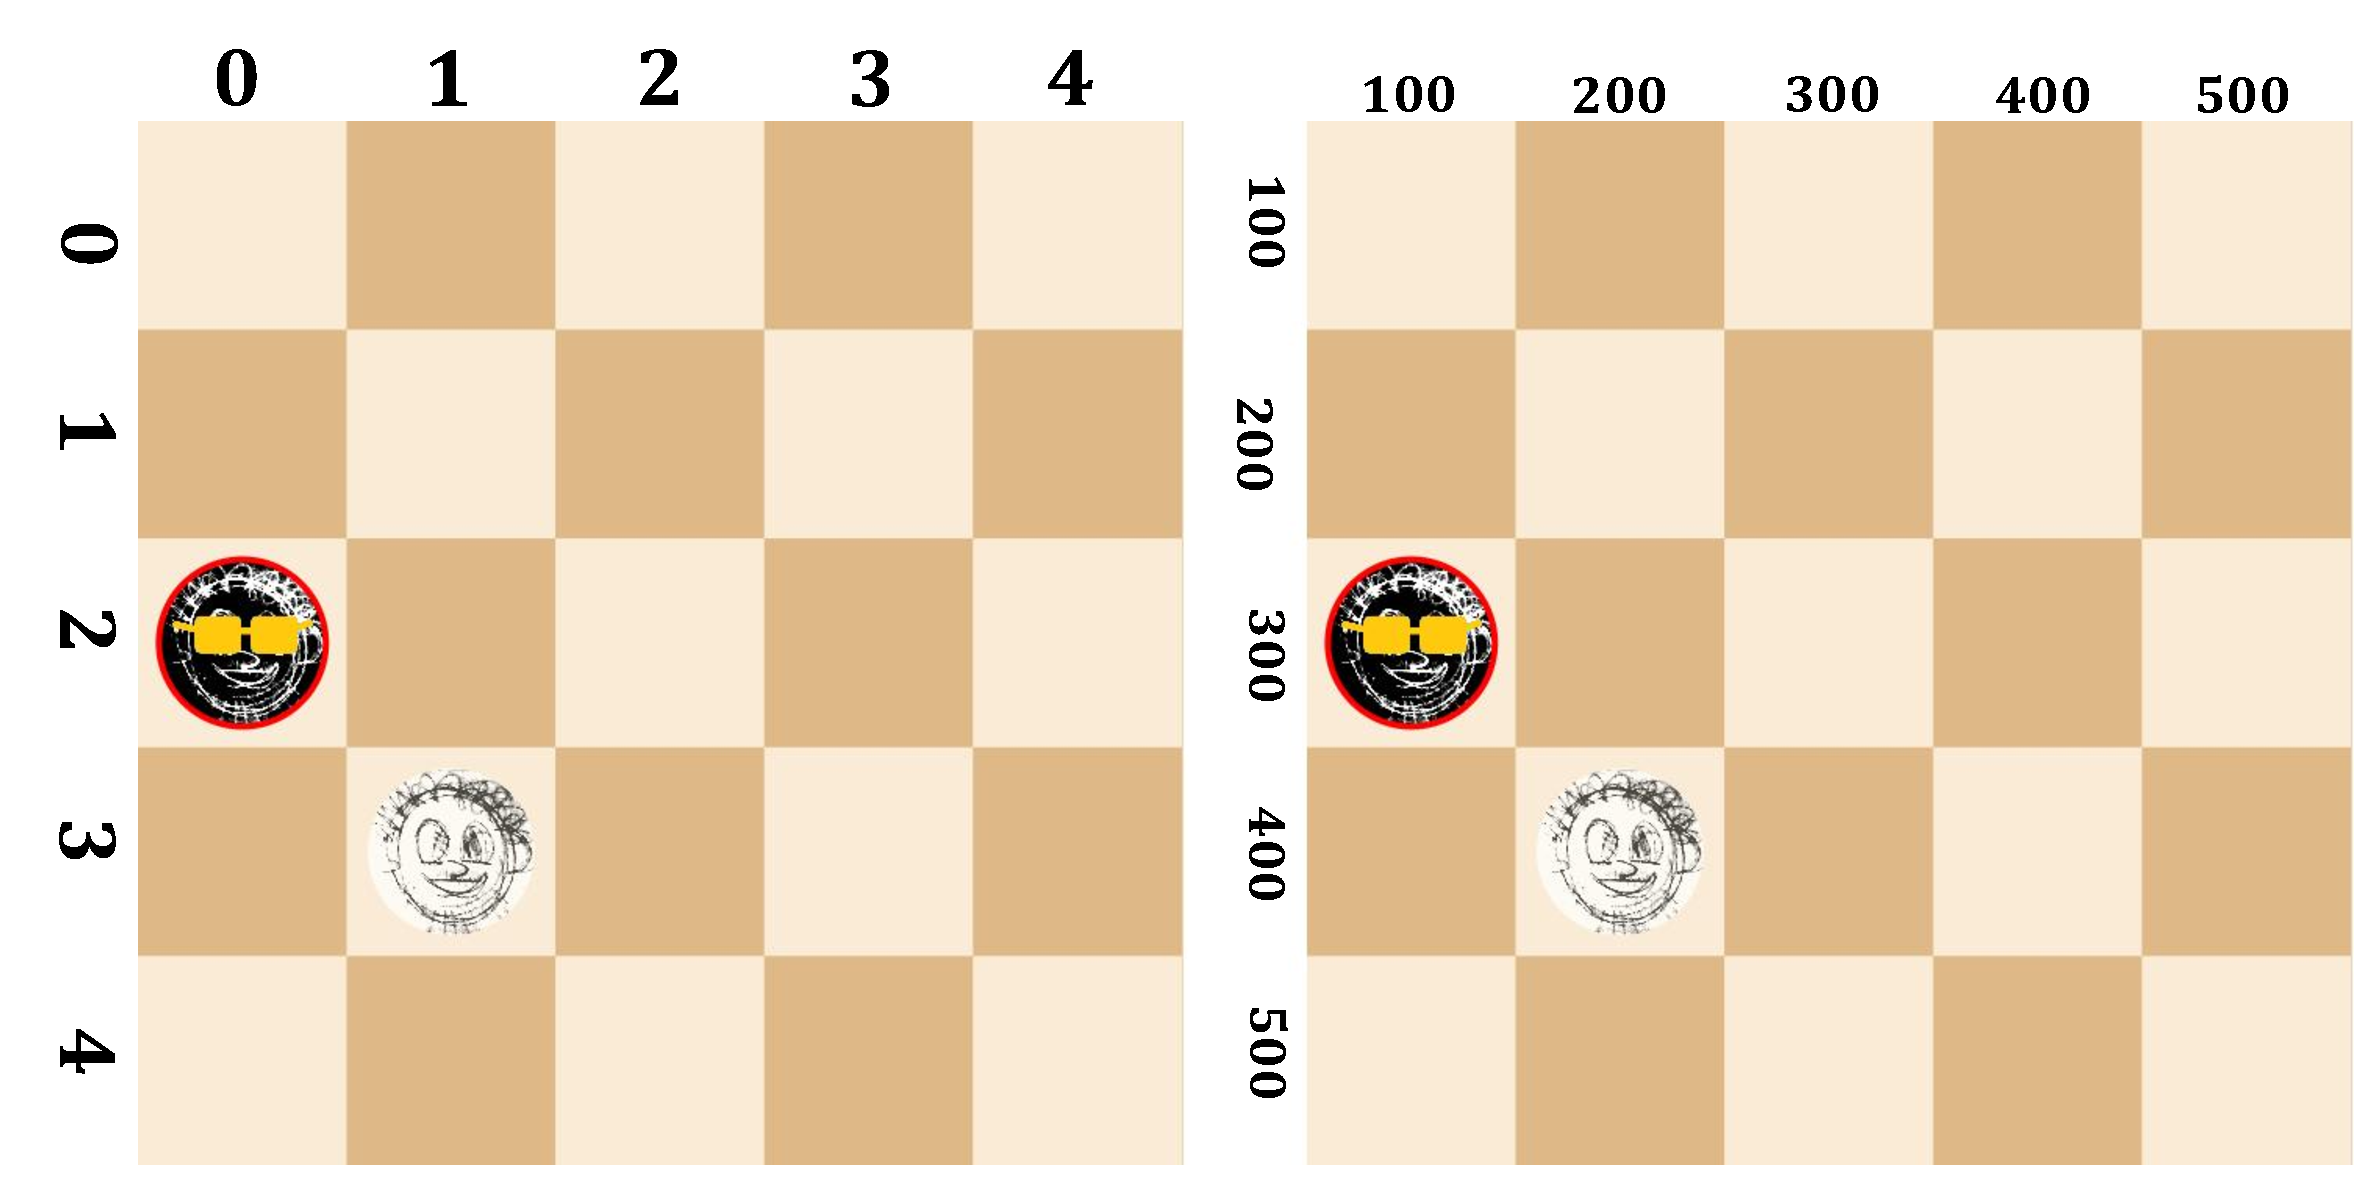
\includegraphics[width = 0.8 \textwidth]{Figurer/modelCoordViewCoord.pdf}
\caption{Model koordinater sammenlignet med View koordinater. Bemærk, at View koordinater varierer fra skærm til skærm, og koordinaterne her svarer blot til én computers koordinater.}
\label{fig:modelCoordViewCoord}
\end{figure}

% Mikkel
\textbf{Brikker:} Brikkerne lagres i en \texttt{ArrayList<Piece> pieces}.

Klassen \texttt{Piece} indeholder fields for sine koordinater på brættet, koordinater på skærmen, hvilken spiller den tilhører, dens farve og størrelse (radius). I \texttt{Piece} findes også metoden \texttt{move}, der håndterer flytning af brikken. Brikkerne sættes op ved metoden \texttt{setupPieces}. \texttt{setupPieces} kører metoden \texttt{placePiece}, og skaber to \texttt{pieces}, i hvert deres hjørne af brættet, og sætter deres hold. Deres positioner bliver sat ud fra \texttt{tileAmount}, så de står i hjørnerne uafhængigt af størrelsen af brættet. Metoden \texttt{placePiece} tager et objekt af typen \texttt{Piece}, og tilføjer det til \texttt{ArrayListen pieces}. Derudover tilføjer \texttt{placePiece} brikken til layoutet, og gør brikkens felt optaget.

\subsubsection{Control}

%% MIKKEL %%
% Hvordan og hvornår opdateres modellen?
% Hvordan dræbes brikker? Bliver de slettet eller skjult?
\textbf{Opdatering af modellen:} Brættet opdateres af metoden updateBoard i klassen \texttt{Control}. Når en brik er blevet flyttet, sætter \texttt{updateBoard} det brikkens nye felt optaget, og det tidligere felt frit.

Når en brik dræbes, køres metoden \texttt{removePiece} fra \texttt{DamModel}. \texttt{removePiece} sletter den dræbte brik fra \texttt{ArrayListen pieces}, fjerner brikken fra \texttt{Layoutet root}, og sætter brikkens tidligere felt til frit. Herefter skiftes fieldet \texttt{turnPlayer} værdi til den anden spiller. \texttt{turnPlayer} starter med at være \texttt{Player.Upper}, svarende til spilleren med de sorte brikker.\\

%% MIKKEL %%
% Hvordan styres et helt træk med en brik
\textbf{Legalt træk:} Når en brik slippes, køres metoden \texttt{isLegalMove} i klassen \texttt{Control}. \texttt{isLegalMove} afgør om trækket var legalt ved brug af metoderne i figur \ref{fig:tjekliste}:


\begin{figure}[H]
\centering
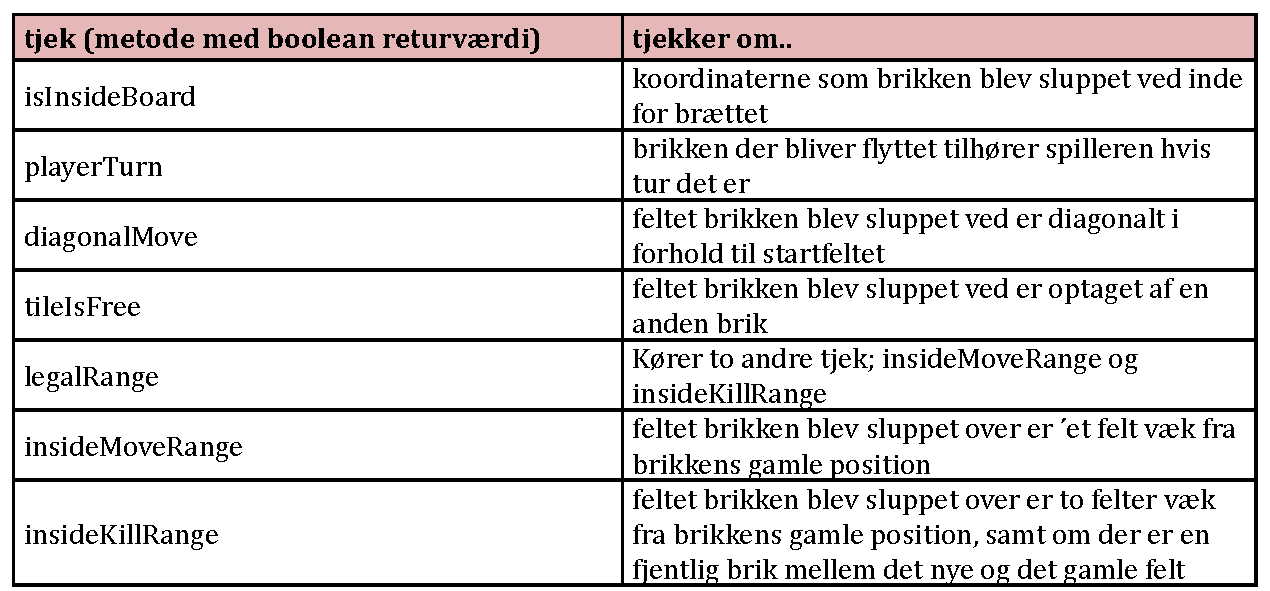
\includegraphics[width = 1.0  \textwidth]{Figurer/tjekliste.pdf}
\caption{Alle de forskellige tjek der bliver kørt i \texttt{isLegalMove}, og hvad de tjekker.}
\label{fig:tjekliste}
\end{figure}

De fleste at metoderne i figur \ref{fig:tjekliste} er accessors, der returnerer booleans. Metoden \texttt{insideKillRange} adskiller sig ved ikke blot at returnere en værdi, men også at være en mutator. Først tjekkes, om feltet mellem slutfeltet og startfeltet er optaget. Hvis dette er sandt, køres et \texttt{for-loop} over \texttt{ArrayListen pieces}, indtil der findes en brik med de feltets koordinater. Denne bliver nu gemt som \texttt{enemyPiece}. Derefter tjekkes, om strækningens længde er legal, og om \texttt{enemyPiece} tilhører fjendens hold. Dette tjek bliver gemt i en boolean \texttt{killPossible}. 

Hvis alle de tjeks i figur \ref{fig:tjekliste} er sande sættes boolean \texttt{moveIsLegal} til sand, så må brikken flyttes. Brættet opdateres.


\subsection{\textsc{AvaDam}}\label{sec:ImpAva}
\subsubsection{View}

\begin{figure}[H]
\centering
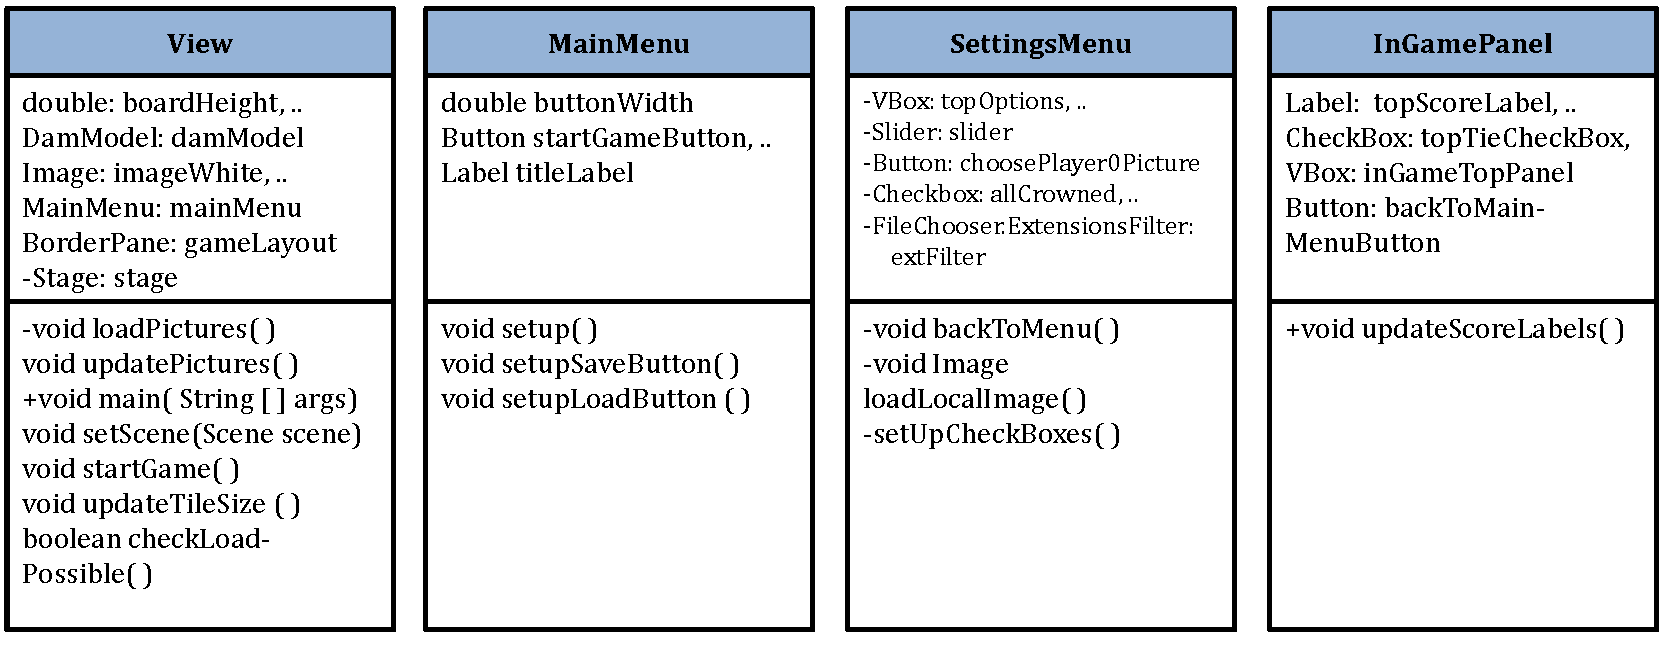
\includegraphics[width = 1.0  \textwidth]{Figurer/classesView.pdf}
\caption{Klassediagram over de klasser der bliver brugt i View-delen af MVC designmønstret.}
\label{fig:classesView}
\end{figure}

%   RR
%\item Hvordan startes spillet? (method calls)
\textbf{Spil startes:} 
Det første der sker når programmet startes, er at de forskellige scener bliver sat op og main menu scenen (\texttt{mainMenuScene}) bliver hæftet til \texttt{JavaFX Applications}'s \texttt{Stage}. I hver scene hæftes de brugte Layouts og modeller. Da \texttt{mainMenuScene} er den første aktive scene, startes spillet altså i main menuen. Derfra har man fri adgang til indstillinger og spillet selv. Ved at trykke på \texttt{"Start new game"} knappen bliver \texttt{gameScene} gjort aktivt og spillet startes med de valgte indstillinger (eller standard indstillinger hvis intet er valgt). \\

Knappen \texttt{"Start new game"} kører metoderne \texttt{startGame}, \texttt{setScene(gameScene)} og \texttt{resetValues} fra henholdsvis \texttt{View} og \texttt{Control} klasserne, hvilket sørger for at spil modellen dannes, spillets scene vises og nødvendige in-game værdier bliver nulstillet. På den måde er knappens funktion uafhængig af om den trykkes når spillet startes, eller efter adskillige spil, da modellen altid startes på ny. 

\begin{figure}[H]
\centering
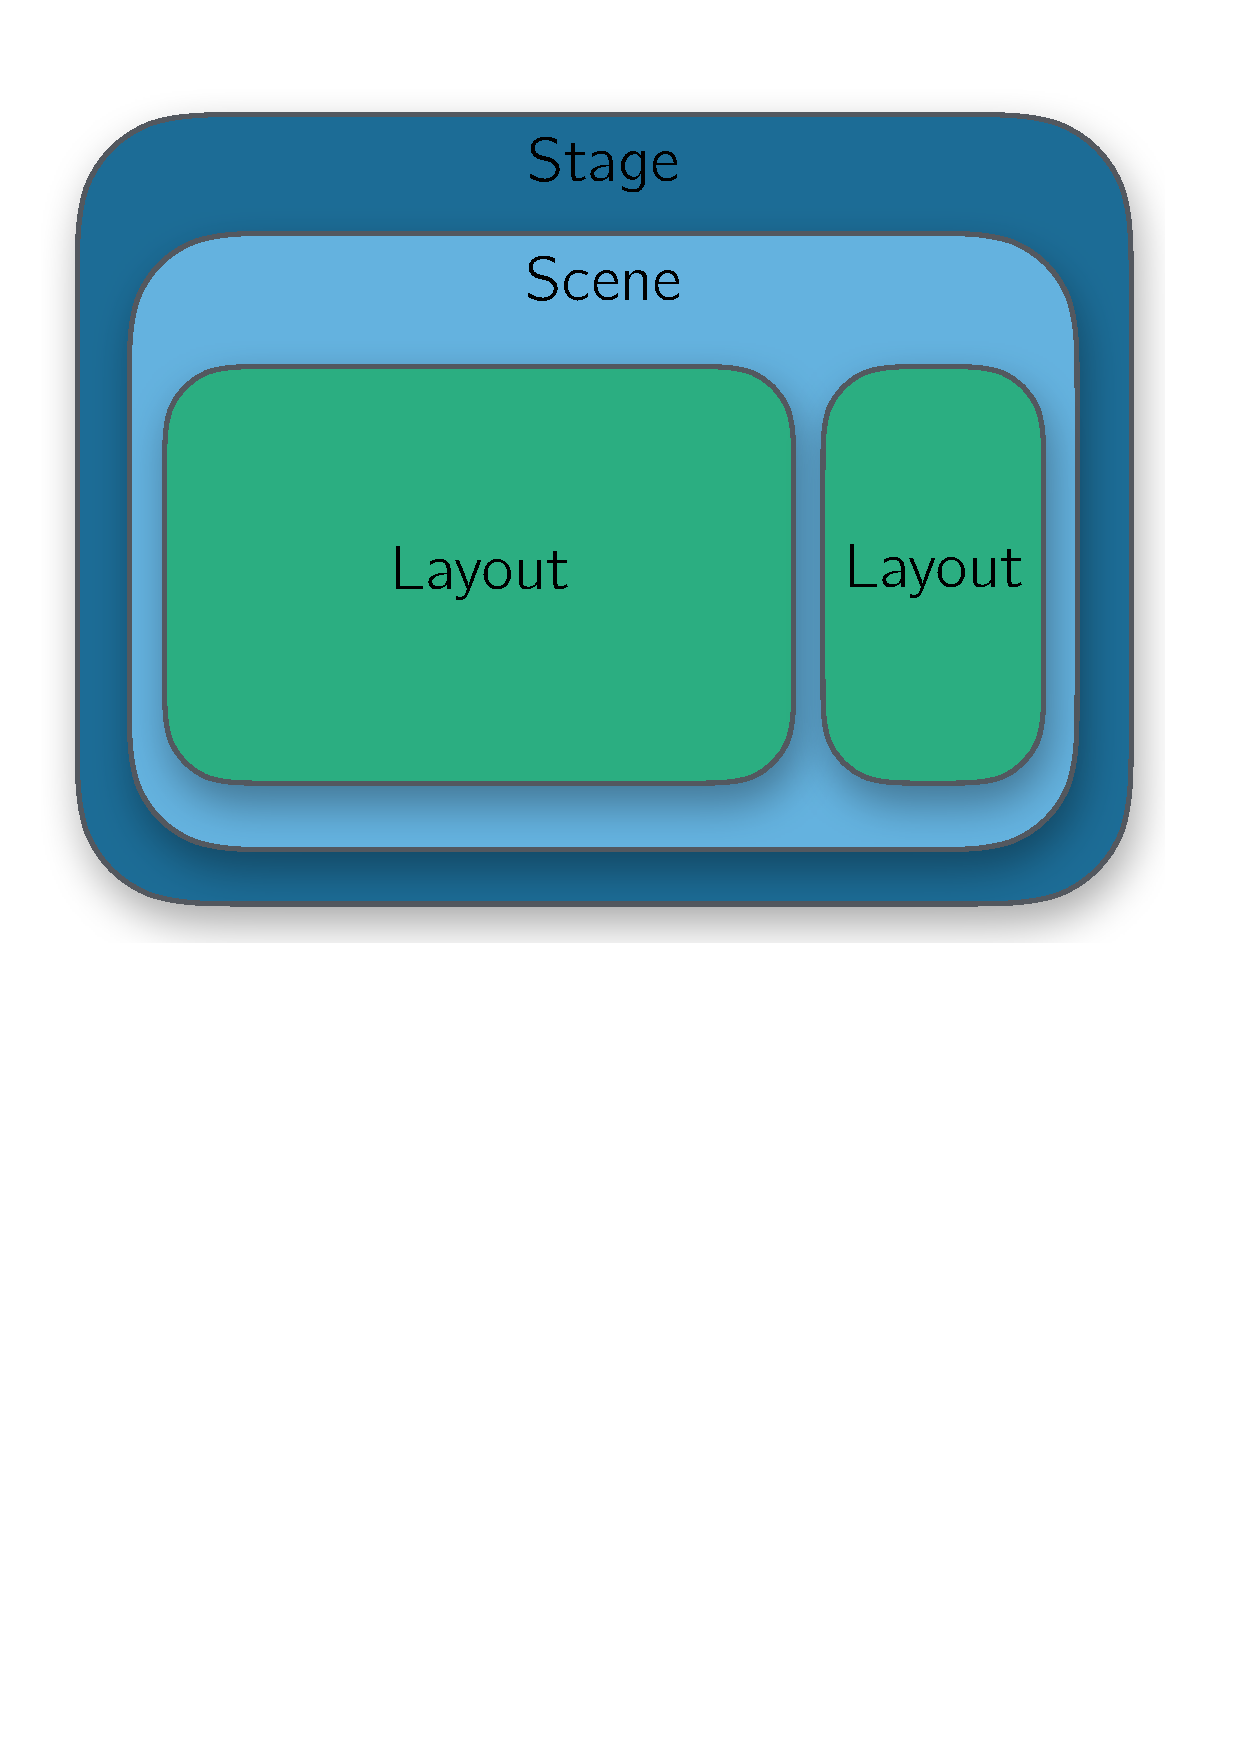
\includegraphics[width = 0.5\textwidth]{Figurer/GUI.pdf}
\caption{Forhold mellem Stage, Scene og Layout i JavaFX.}
\label{fig:GUI}
\end{figure}

%   RR
%\item Hvordan håndteres brug af scenes?    
\textbf{Scenes:} 
Vi bruger følgende scenes: \texttt{mainMenuScene}, \texttt{settingsScene} og \texttt{gameScene}. Hver scene repræsenterer et segment af programmet, og for at skifte fra fx menuen med indstillinger til main menu, skiftes fra \texttt{settingsScene} til \texttt{mainMenuScene} direkte i \texttt{JavaFX Applications}'s \texttt{Stage} via \texttt{stage.setScene(mainMenuScene)}. Scenen kan også fra andre klasser ved brug af \texttt{View.setScene(Scene scene)}.\\

%Jens
%Hvordan bruges I styles og CSS?
\textbf{Cascading Style Sheets:} Stilen og udseende af de tre forskellige scener: \texttt{gameScene}, \texttt{settingsScene} og \texttt{mainMenuScene}, bliver sat af tre korresponderende \texttt{.css} filer med tilsvarende navne via fx \texttt{.getStyleSheets().add("GameScene.css")}. Ved brug af stylesheets bliver bla. skriftyper og størrelser, baggrundsfarve, tekstfarve mm. indstillet. Syntaksen og formen af \texttt{.css} filer gør det nemt at ændre hele sceners udseende hurtigt og bidrager til høj fleksibilitet og overskuelighed til programmets udseende. CSS er især brugbart til større programmer.\\

%Jens
%Hvordan håndteres user input?
\textbf{Bruger input:} Al interaktion med brugeren af programmet håndteres gennem listeners som sætter gang i forskellige events. \texttt{JavaFX} har som standardindstilling listeners til piletasterne og mellemrum aktiveret. Dette gør menunavigering nemmere, da mellemrum bla. sætter gang i et \texttt{setOnKeyPressed()} event for en markeret knap, og piletasterne skifter mellem hvilken knap der er markeret. Udover dette har vi gjort brug af fire yderligere forskellige slags listeners. Den første er tilføjet til \texttt{gameScene} og \texttt{settingsScene}; en \texttt{setOnKeyPressed} listener der, hvis den trykkede knap er Esc, skifter den viste scene ud med hovedmenuen. De sidste tre er til museinteraktionenerne pressed, dragged og released, som bliver brugt til at flytte brikker. Disse listeners aktiveres i \texttt{Piece}-klassens konstruktør under metoden \texttt{move}.
\begin{lstlisting}
void move() {
    setOnMousePressed(mouse -> {
        startThisPiece(this);
    });
    setOnMouseDragged(mouse -> {
        updateThisPiece(this, mouse);
    });
    setOnMouseReleased(mouse -> {
        if (hasLegalEndPosition(this)) {
            finishThisPiece(this);
            startNextTurn();
        } else {
            continueThisPiece(this);
    	}
        updateAllPieces();
        updateAllTiles();
        runAI();
    });
}
\end{lstlisting}
De kaldte metoder ovenfor findes i \texttt{Control} og \texttt{TopLevelControl}. \\

% Magnus
% Hvordan skiftes mellem billeder af ikke-fokus brik, valgt brik, og kronet brik? (adv)
\textbf{Skift af billeder (valgt, kronet):} Når en brik trækkes med musen eller krones, opdateres brikkens billede. I \texttt{TopLevelControl} findes metoden \texttt{updateThisPiece}, der køres når en brik trækkes:
\begin{lstlisting}
static void updateThisPiece(Piece piece, MouseEvent mouse) {
// If not crowned, change between normal and chosen 
if (!piece.getCrowned()) {
piece.setFill(piece.player == Player.Upper ? blackChosen : whiteChosen); } } }
\end{lstlisting}

\texttt{blackChosen} og \texttt{whiteChosen} er \texttt{ImagePatterns} i \texttt{View} klassen, der repræsenterer billederne i figur \ref{fig:defaultPieces}.  \\

%% MIKKEL %%
% GULD RING???????
\textbf{Guld ring:} Guld ringen, der indikerer om en brik er kronet, sættes på to forskellige måder. Hvis en brik bliver kronet i sin konstruktør, bliver kantfarven sat til guld via fieldet \texttt{crownedColor}. Når en brik når til modstanderens bageste række, bliver brikken kronet via metoden \texttt{finishThisPiece}. Et eksempel på dette er: 

\begin{lstlisting}
if (selectedPiece.player == Player.Upper && releasedAtY == tileAmount - 1) {
	selectedPiece.setCrowned(true);
	selectedPiece.setFill(View.blackCrowned);
	selectedPiece.setStroke(Color.GOLD);
}
\end{lstlisting}

%% MIKKEL %%
% Hvordan er rød og guld ring implementeret?
\textbf{Rød ring:} Når en brik slippes, køres metoden \texttt{updateAllPieces}. \texttt{updateAllPieces} kører en række andre metoder, nogle af hvilke vil blive beskrevet nedenfor.

\begin{enumerate}
    \item Metoden \texttt{checkPossibleKills} hvis \texttt{mandatoryFirstKill} er sat til. \texttt{checkPossibleKills} kører et loop over alle brikker i \texttt{pieces}, og kører metoden \texttt{canKill} på dem.
    
    \item \texttt{canKill} tager imod et \texttt{Piece} og tjekker, om brikken kan dræbe i hver af de retninger der er tilgængelige for den gennem metoden \texttt{canKillThisDirection}.
    
    \item \texttt{canKillThisDirection} tager imod et \texttt{piece}, samt modelkoordinater \texttt{dx} og \texttt{dy}, der betegner hvilke koordinater der skal tjekkes, relativt til brikkens egne modelkoordinater. \texttt{canKillThisDirection} returnere en boolean, der er sand hvis der er en brik på feltet betegnet gennem \texttt{dx} og \texttt{dy}, hvor den fjendtlige brik er af et andet hold en den valgte brik, samt at feltet efter den fjendtlige brik er ledigt. 
    
    \item Hvis alle disse er sande, returnerer \texttt{canKillThisDirection} sand, og sætter \texttt{canKill} til true på den valgte brik gennem metoden \texttt{setCanKill}. 
    
    \item \texttt{setCanKill} tager en boolean som argument, og hvis denne er true, sætter den brikkens \texttt{stroke} til rød, gennem fieldet \texttt{killColor}. Hvis den tager imod boolean false, sætter den enten brikkens stroke til guld, hvis den er kronet, ellers sætter den stroke til transparent.
   
\end{enumerate}

% Magnus
% Hvordan animeres spawn og død? 
\textbf{Animation af spawn\footnote{Med begrebet spawn menes: Hændelsen hvor en ny brik bliver placeret på brættet.} og død:} Animationen af spawn og død er implementeret ved brug af \texttt{ScaleTransition}. Animationen sker når der skiftes scene. Brikker bliver markeret som kronet ved at deres \texttt{isCrowned} field opdateres, så animationen sker ikke, når brikker krones; det er samme brik. Animation af død er implementeret i klassen \texttt{DamModel}, da det er integreret i \texttt{removePiece} metoden, der først skalerer brikken ned (visualiserer død), derefter fjerner brikken fra dens tilhørende \texttt{tile} (via \texttt{setPiece(null)}), endeligt fjernes den visuelt fra skærmen via \texttt{getChildren().remove(piece)}.

\begin{figure}[H]
\centering
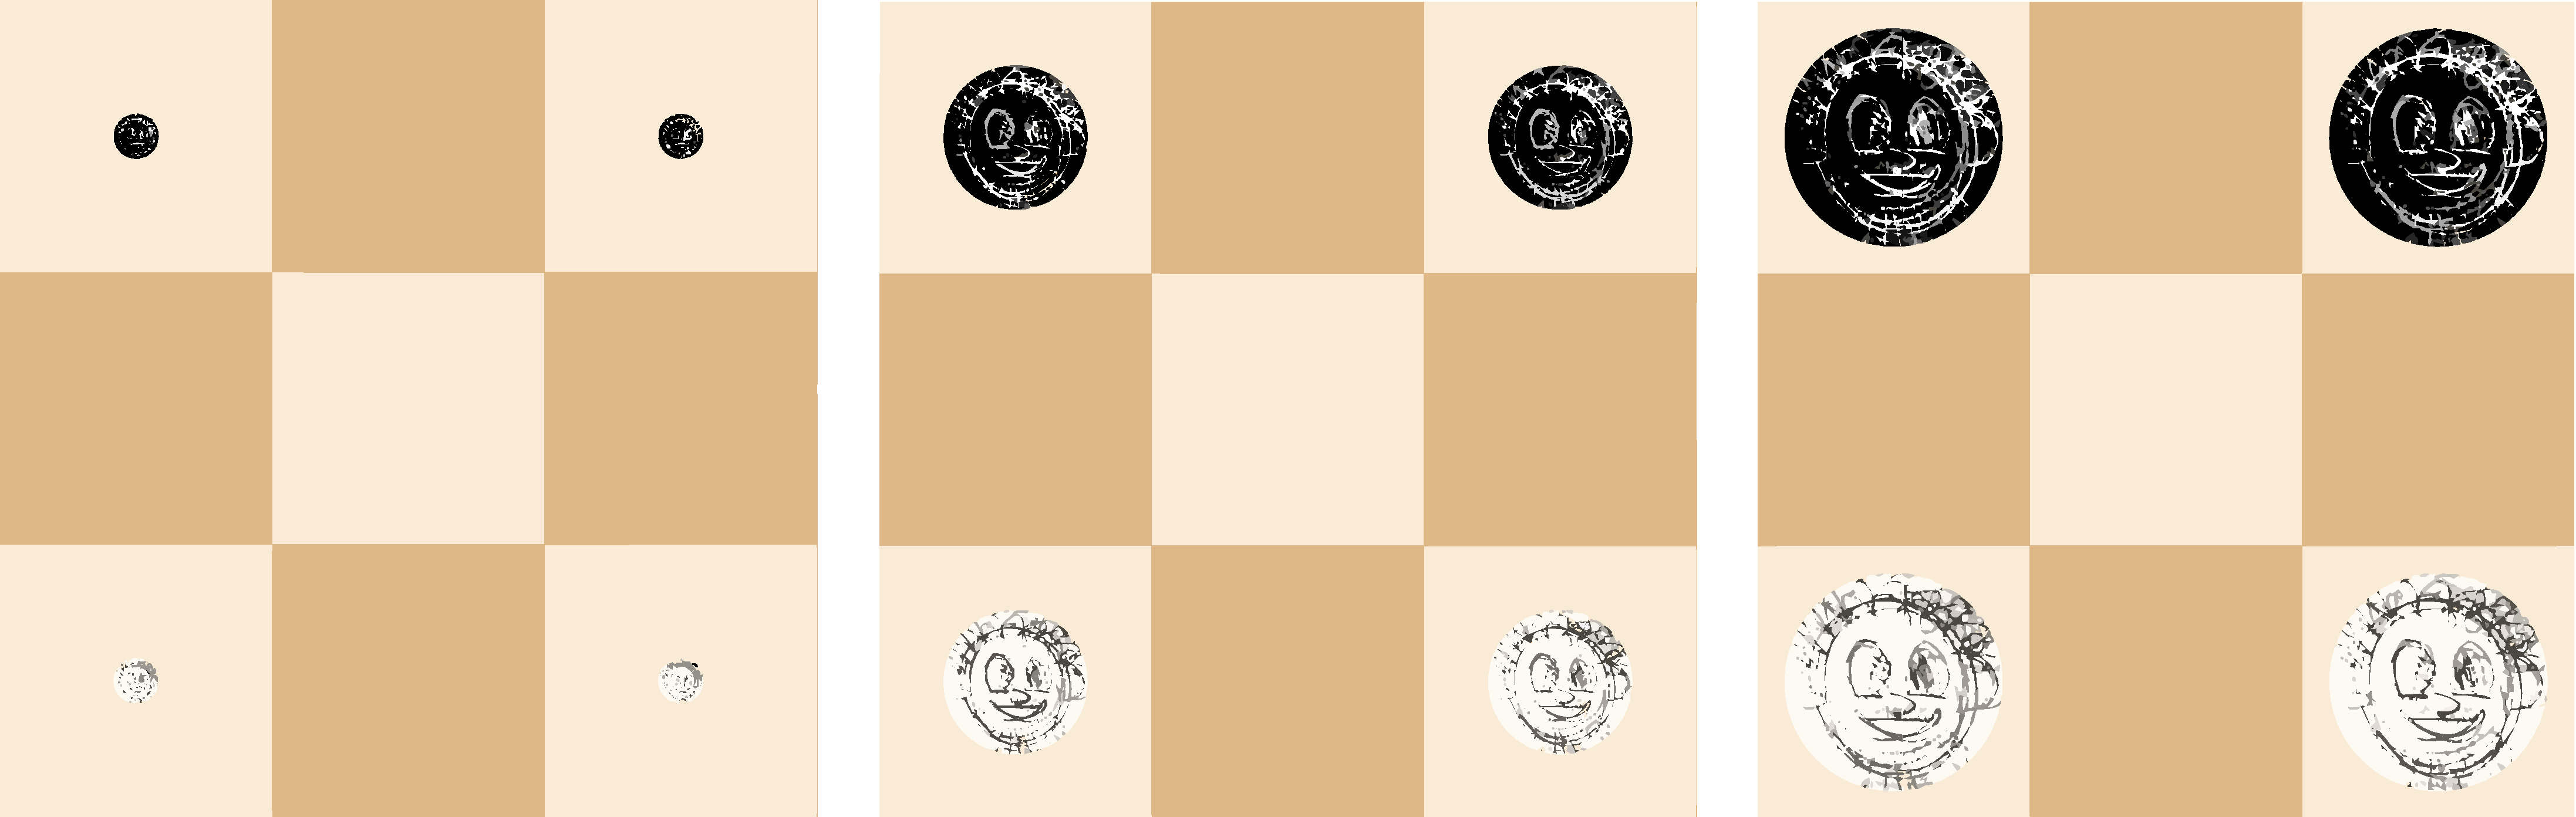
\includegraphics[width = 0.8  \textwidth]{Figurer/spawn.pdf}
\caption{Animation af hvordan brikker spawnes på brættet. Brikkerne skaleres fra et punkt op til deres aktuelle størrelse over et forløb på 600 millisekunder.}
\label{fig:spawn}
\end{figure}


\subsubsection{Model}
\vspace{-0.5cm}
\begin{figure}[H]
\centering
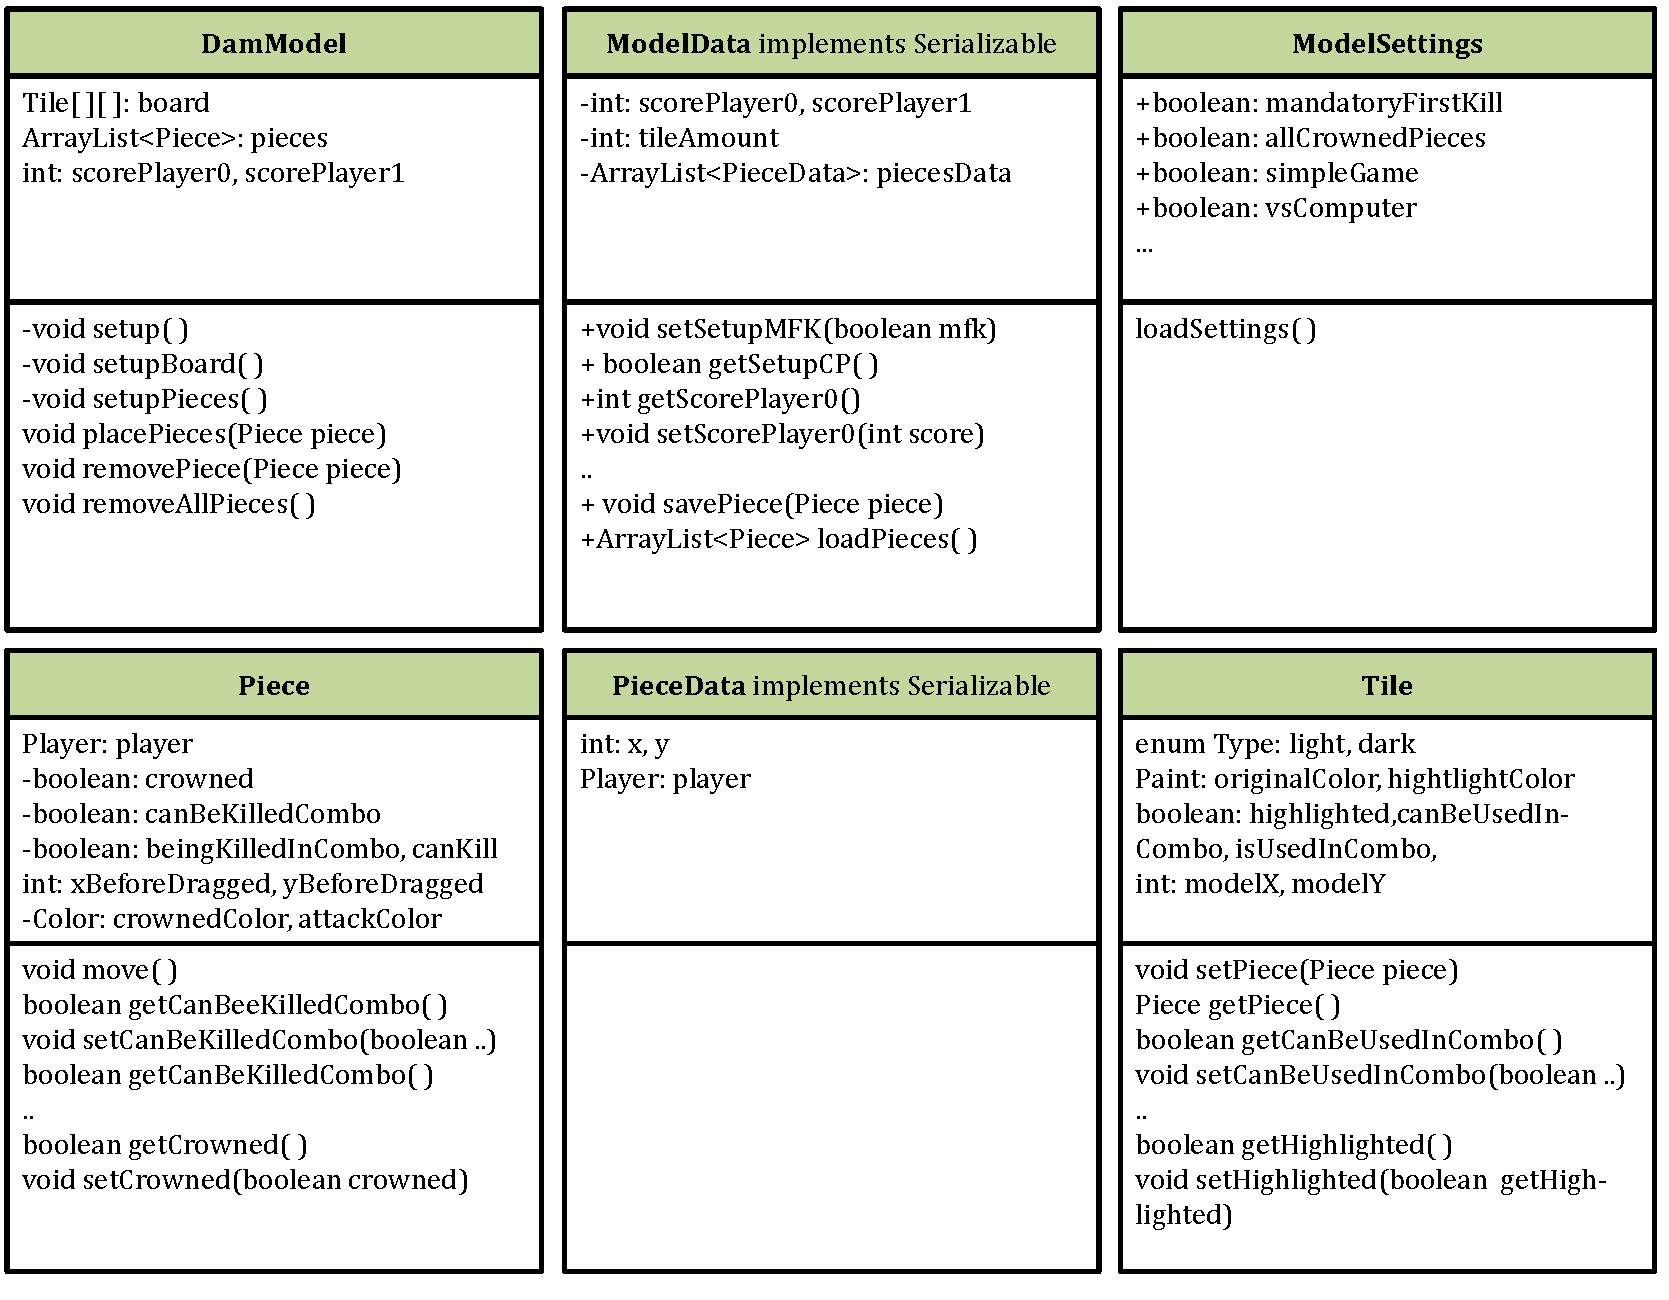
\includegraphics[width = 1.0  \textwidth]{Figurer/classesModel.pdf}
\caption{Klassediagram over de klasser der bliver brugt i Model-delen af MVC designmønstret.}
\label{fig:classesModel}
\end{figure}

%% MIKKEL %%
% BRÆT????
\textbf{Brættet:} I forhold til \textsc{SimpDam} er der tilføjet følgende booleans til felter af typen \texttt{Tile}: \texttt{highlighted}, \texttt{canBeUsedInCombo} og \texttt{isUsedInCombo}. I stedet for brug af et boolean \texttt{occupied}som i \textsc{SimpDam}, har hvert felt nu direkte forbundet med sin tilhørende brikken. Brættet lagres stadig i \texttt{Tile[][] board}. \\

%% MIKKEL %%
% Hvordan lagres brikker og tiles internt?
\textbf{Brikker:} \texttt{Piece} i \textsc{AvaDam} er en udbygning af \texttt{Piece} i \textsc{SimpDam}: Der er tilføjet følgende booleans:  \texttt{crowned}, \texttt{canKill}, \texttt{canBeKilledInCombo}, \texttt{beingKilledInCombo}. Udover disse har \texttt{Piece} også to farver \texttt{crownedColor} og \texttt{killColor}, der bruges til at sætte kantfarver, samt et felt \texttt{Player}. Vi har tilføjet en \texttt{player} \texttt{None}, svarende til at ingen må flytte brikker (fx når spillet er ovre.) Konstruktøren for brikken tager nu også imod om brikken er kronet. Brikker lagres stadig i ArrayListen \texttt{<Piece> pieces}, og fjernes som i \textsc{SimpDam}. \\

%% MIKKEL %%
% Hvordan lagres spilreglerne?
\textbf{Valgfri regler:} De valgfri regler kan ændres i Settings menuen. Klassen \texttt{ModelSettings} indeholder booleans svarende til disse regler, som set i \ref{fig:settingsMenu}. Når en \texttt{CheckBox} i settings menuen bliver trykket på, opdateres den tilsvarende boolean i \texttt{ModelSettings}. Nogle check boxes sætter flere værdier, såsom \texttt{mustCompleteCombo} der også sætter \texttt{mandatoryFirstKill} til sand (og gør dennes \texttt{CheckBox} inaktiv), da et drab er en combo med længden 1. \\

Når brugeren klikker \texttt{"Start game"}, bruges indstillingerne fra \texttt{ModelSettings} til konstruktørerne af bræt og brikker. Dette udføres af metoden \texttt{loadSettings}. 

Når sliderens værdi ændres i menuen med indstillinger, opdateres den tilknyttede label ved brug af følgende kode:
\begin{lstlisting}
slider.valueProperty().addListener((obs, oldVal, newVal) -> {
    sliderValueLabel.setText("" + (int) slider.getValue());
});
\end{lstlisting}

Dens værdi bliver overført til \texttt{tileAmount} når metoden \texttt{setup} bliver kørt i \texttt{DamModel}, hvor den bliver overført til \texttt{tileAmount} gennem \texttt{slider.getValue}. 

\begin{figure}[H]
\centering
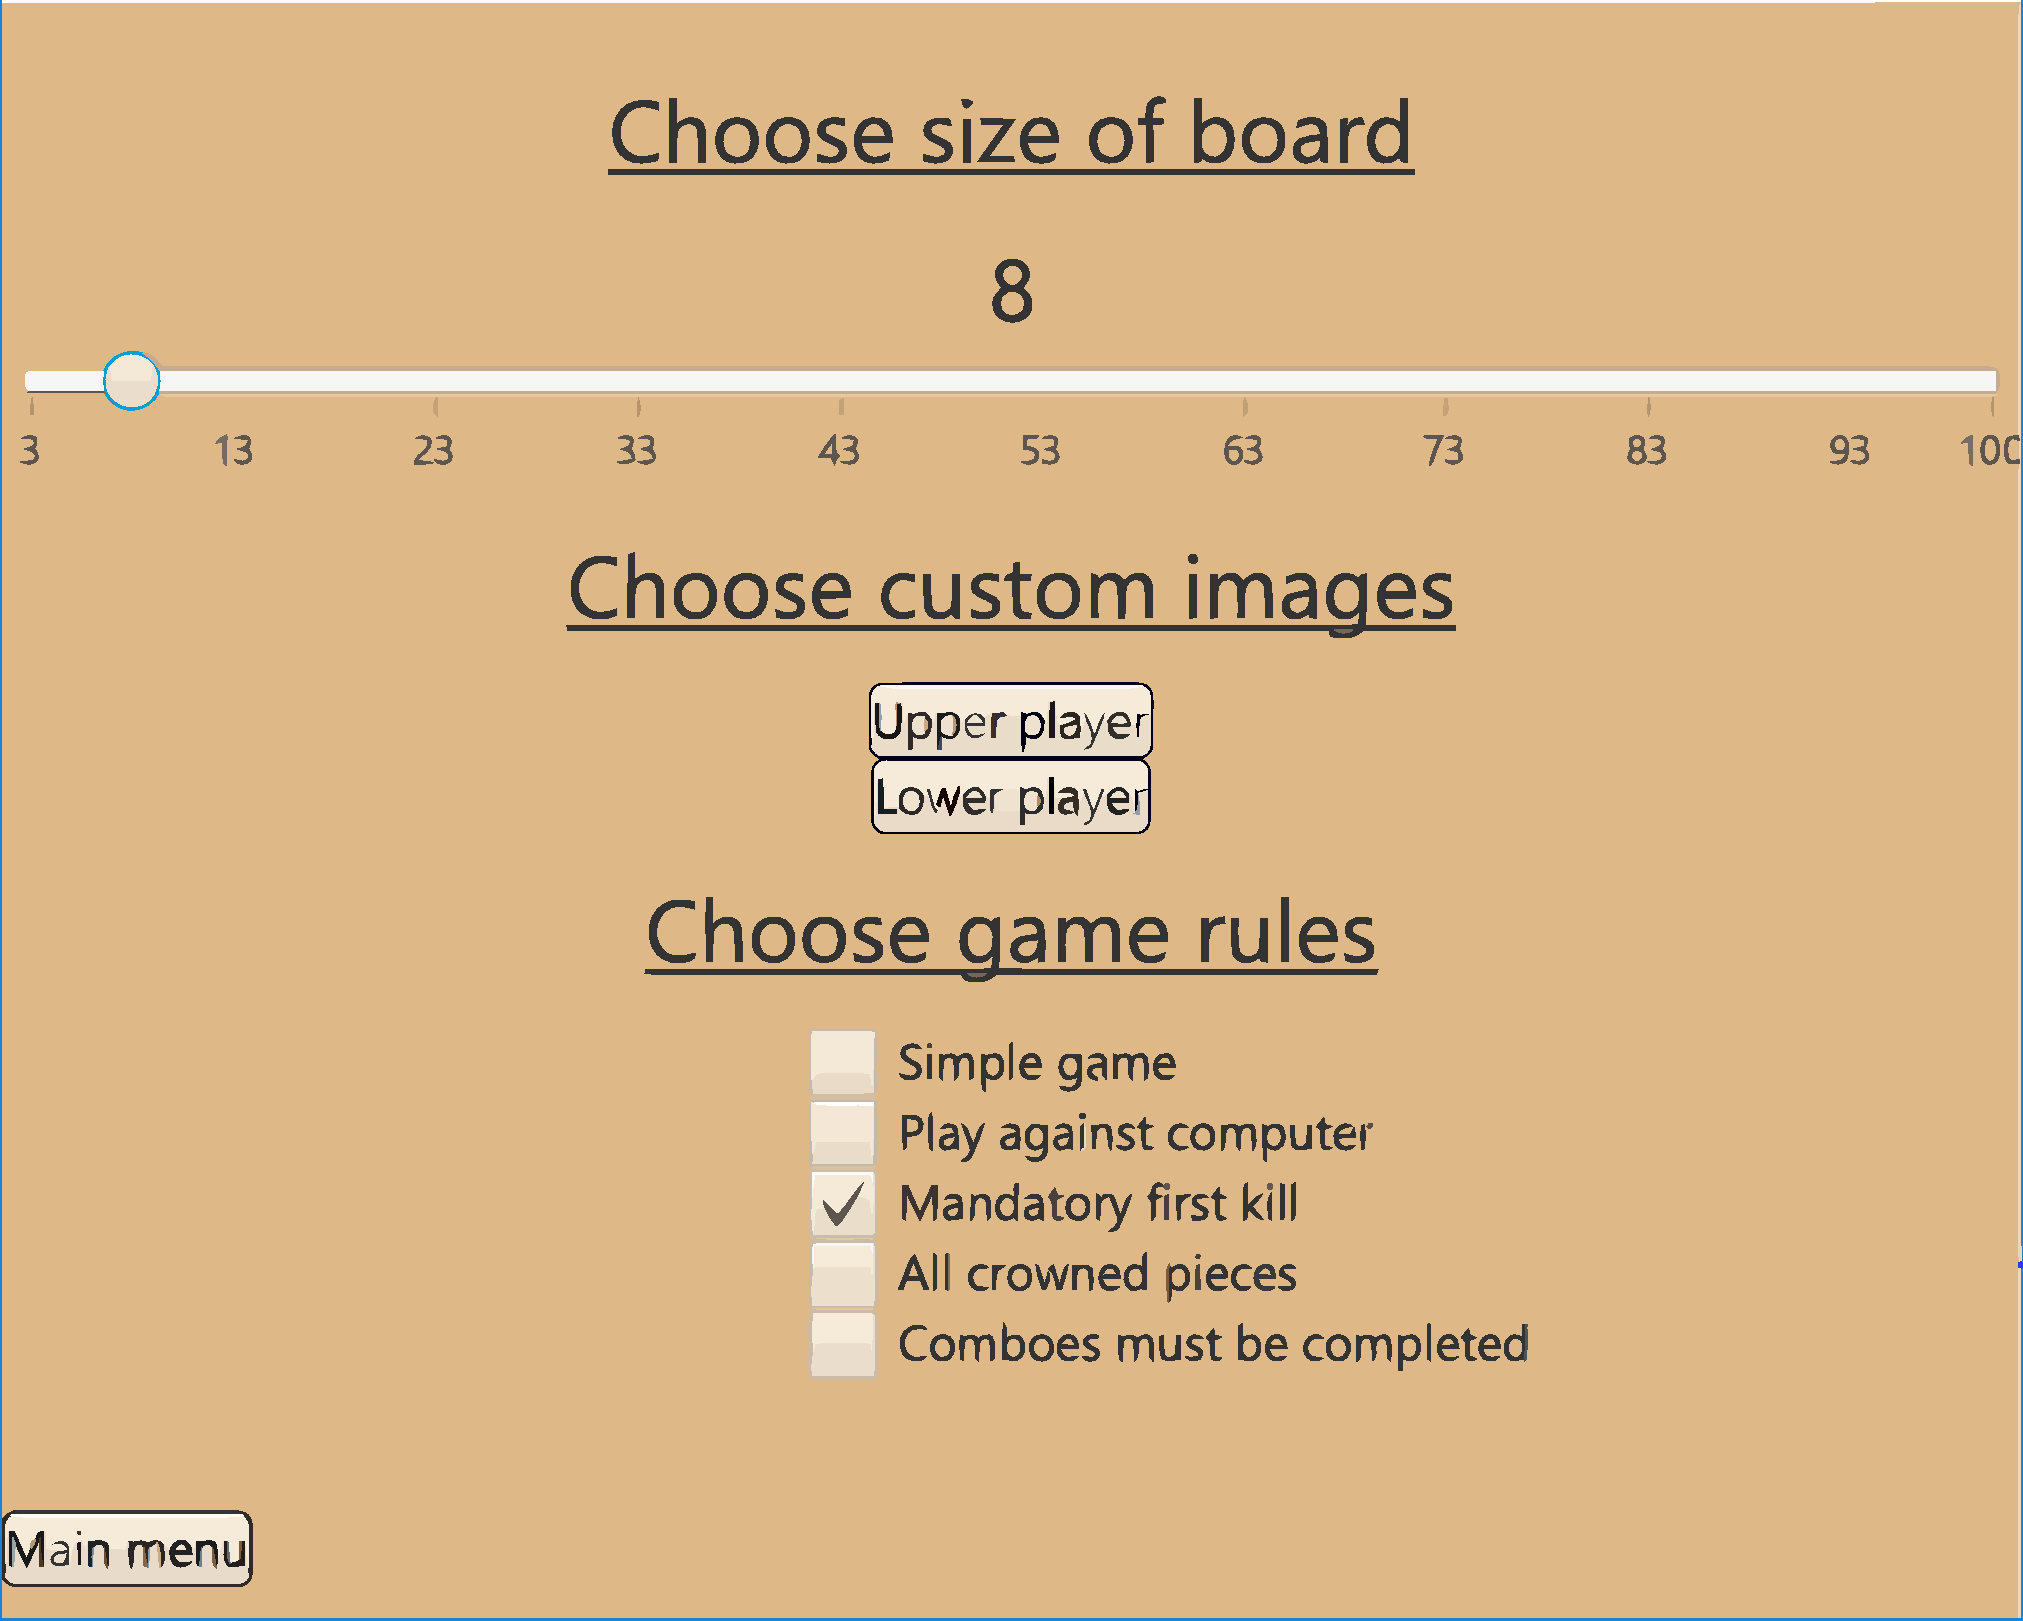
\includegraphics[width = 0.7\textwidth]{Figurer/settingsMenu.pdf}
\caption{Menuen for indstillinger. Her kan vælges brætstørrelse, brikbilleder og diverse spilindstillinger.}
\label{fig:settingsMenu}
\end{figure}
\subsubsection{Control}
\begin{figure}[H]
\centering
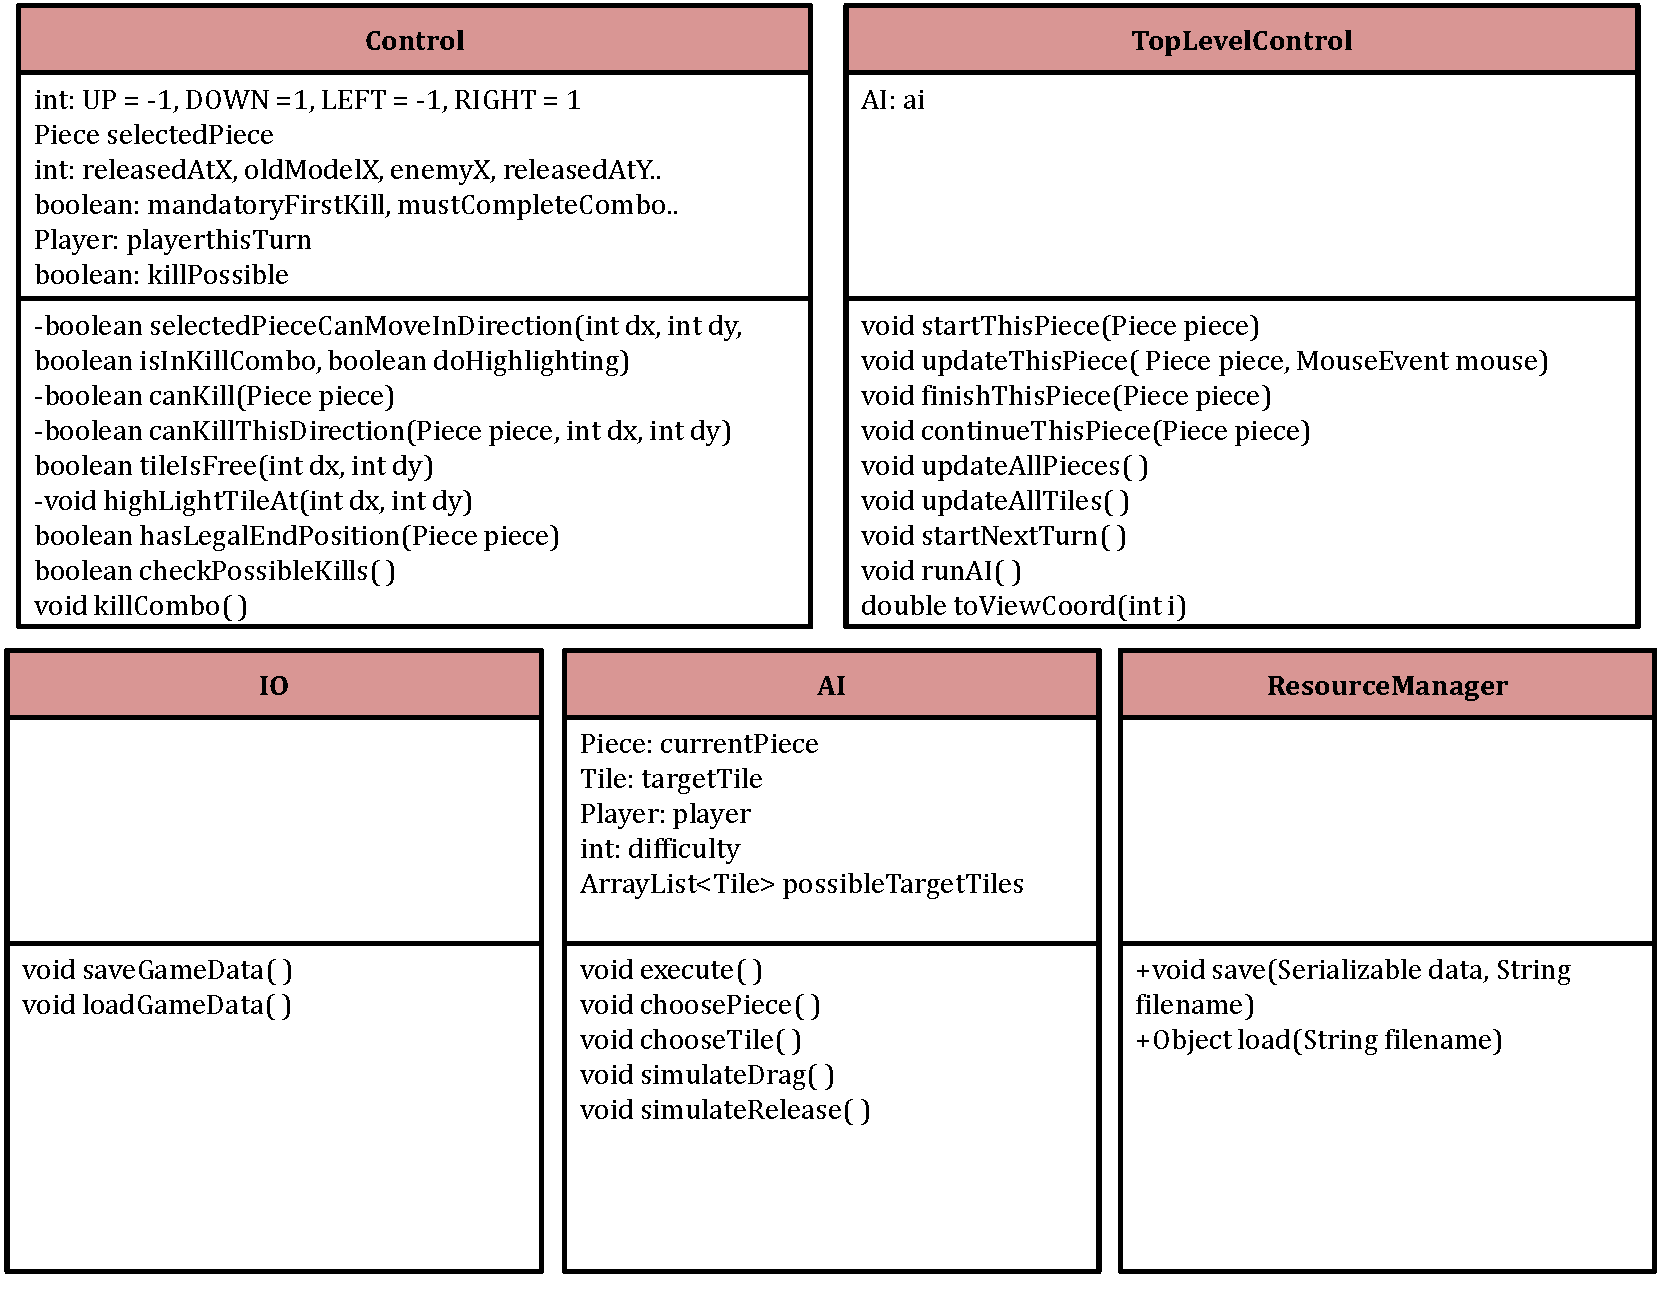
\includegraphics[width = 1.0  \textwidth]{Figurer/classesControl.pdf}
\caption{Klassediagram over de klasser der er med i Control-delen af MVC designmønstret.}
\label{fig:classesControl}
\end{figure}
%   RR
%    \item Hvordan og hvornår opdateres modellen? 
\textbf{Opdatering af modellen:} 
Det er valgt, at modellen kun opdateres når der har været brugerinteraktion med en brik. Opdateringen sker gennem \texttt{TopLevelControl} med metoderne: 

\begin{lstlisting}
    startThisPiece(Piece piece) { ... }
    updateThisPiece(Piece piece, MouseEvent mouse) { ... }
    continueThisPiece(Piece piece) { ... }
    finishThisPiece(Piece piece) { ... }
    startNextTurn() { ... }
    updateAllPieces() { ... }
    updateAllTiles() { ... }
    runAI(){ ... }
\end{lstlisting}


\begin{enumerate}
    \item Når en brik bliver valgt, kaldet det pågældende \texttt{Piece} instans metoden \texttt{startThisPiece} i \texttt{TopLevelControl}. Ved at kalde \texttt{startThisPiece} vil mulige træk blive fundet gennem \texttt{Control} klassen.
    
    \item Når brikken trækkes med musen køres \texttt{updateThisPiece(this, mouse)}\footnote{I dette tilfælde er \texttt{mouse} et \texttt{MouseEvent} lavet via et lambda udtryk.} i den samme \texttt{Piece} instans. Ved at kalde \texttt{updateThisPiece} vil brikken følge musen hvis musen er inden for brættet, samt tjekke om brikken er trukket over et felt, der kan indgå i en combo. Hvis brikken trækkes over et sådan felt, fjernes tidligere highlight, det nye felt bliver tilføjet til comboen, og nye mulige træk bliver udregnet fra denne position. Brikkens billede skiftes fra normalt billede til dens \texttt{chosen} billede.
    
    \item Når brikken slippes, kaldes resterende metoder, afhængig af om trækket var legalt eller ej. Hvis trækket var illegalt, køres \texttt{continueThisPiece(this)}, der flytter brikken tilbage til dens udgangspunkt. Hvis trækket var legalt, køres \texttt{finishThisPiece(this)}, der opdaterer brikken til den nye position, tjekker om brikken skal krones og udfører eventuelle drab. 
    % HEJ MAGNUS %%%% %%%%%
    \item Efter \texttt{finishThisPiece} køres \texttt{startNextTurn} som skifter spiller, nulstiller fields og tjekker om der findes et gyldigt træk for den nye spiller. I tilfældet af intet gyldigt træk findes, er spillet slut.
    
    \item Til sidst køres \texttt{updateAllPieces}, \texttt{updateAllTiles} og \texttt{runAI}, hvilket sørger for at brættet er klart til den nye spiller, og lader AI'en spille for modstanderen i tilfældet af at det er valgt i indstillingerne. 
\end{enumerate}

%   RR
%    \item Hvordan highlightes felter?
\textbf{Highlighting af felter:}  
Highlighting af felter er en sideeffekt af en anden proces. Metoderne \texttt{startThisPiece} og \texttt{updateThisPiece} fra \texttt{TopLevelControl} kalder begge metoden \texttt{thisPieceCanMove} i \texttt{Control}. Metoden \texttt{thisPieceCanMove} modtager 3 parametre: \texttt{Piece piece}, \texttt{boolean isInKillCombo} og \texttt{boolean doHighlighting}. 

Parameteren \texttt{isInKillCombo} fortæller \texttt{Control} om brikken allerede har dræbt en fjende i denne tur. Parameteren \texttt{doHighlighting} gør at der skiftes farven på de felter der indgår i brikkens gyldige træk, hvis den er sand. På den måde bruges metoden på flere måder, mens koden er holdt kompakt for at mindske redundans. \\

%   RR
%    \item Hvordan dræbes brikker? Bliver de slettet eller skjult?
\textbf{Drab af brikker:} 

Brikker lagres og dræbes ligesom i \textsc{SimpDam}, med følgende udvidelse: brikken fjernes nu fra dens tilknyttede felt via \texttt{setPiece(null)} i stedet for en boolean \texttt{setOccupied(false)}, og døden animeres ved en \texttt{ScaleTransition} (\texttt{st}). Når animationen er færdig, aktiveres et event via \texttt{st.setOnFinished(event -> \{...\})} som til sidst fjerner brikken fra Layoutet. Alt dette sker i metoden \texttt{removePiece(Piece piece)} i \texttt{DamModel} klassen. Der bliver ikke tjekket direkte om brikken, der dræbes, er en fjende. Det er dog tidligere tjekket, at brikker kun kan placeres på den anden side af en fjende, så et sådan tjek af drab behøves ikke.\\

%   RR
%    \item Hvordan dræbes fjender i comboer? 
%    \item Hvilke fields og methods bruges ved comboer?
\textbf{Drab af brikker i combo:} 
Når flere brikker bliver dræbt via combo, sker det ved brug af \texttt{removePiece} metoden beskrevet ovenfor. Når comboen udføres, bliver medvirkende felters modelkoordinater lagret i en \texttt{ArrayList<Point> comboPositions}. Derefter slettes brikker med modelkoordinaterne svarende til elementerne i \texttt{comboPositions}.\\

%% MIKKEL %%
% Hvordan håndteres og opdateres score label?
\textbf{Score labels:} I layoutet \texttt{inGamePanel} findes bl.a. labels, der indeholder spillernes score. Spillernes score øges via metoden \texttt{incrementScoreBy} i \texttt{Control}. \texttt{incrementScoreBy} tager et heltal som parameter, og tilføjer denne til scoren for den spiller hvis tur det er. Metoden ses i koden nedenfor.
\begin{lstlisting}
static void incrementScoreBy(int increment) {
	if (selectedPiece.player == Player.Upper)
		DamModel.scorePlayerUpper += increment;
	else
		DamModel.scorePlayerLower += increment;

	InGamePanel.updateScoreLabels(); }
\end{lstlisting}

Metoden \texttt{updateScoreLabels} sætter teksten for to labels \texttt{topScoreLabel} og \texttt{bottomScoreLabel}, der vises i toppen af henholdsvis toppen og bunden af \texttt{inGamePanel}. \texttt{updateScoreLabel} tilgår \texttt{scorePlayerUpper} og \texttt{scorePlayerLower} fra \texttt{DamModel}, og sætter teksterne i \texttt{inGamePanel} til disse. Når der startes et nyt spil, køres metoden \texttt{resetAllValues}, der nulstiller scoren.\\

% Magnus
% Hvad sker der når der skiftes tur?
\textbf{Skift af tur:} Når der skiftes tur, opdateres først variablen \texttt{playerThisTurn} i \texttt{Control}, der holder rede på hvis tur det er. Derefter tjekkes alle spillerens brikker mht. om den nye spiller kan flytte en brik. Hvis ikke, har denne spiller tabt.

\begin{lstlisting}
static void startNextTurn() {
playerThisTurn = selectedPiece.player == Player.Upper ? Player.Lower : Player.Upper;	

boolean moveIsPossible = false;		
for (Piece piece : DamModel.pieces) {
  if (piece.player == playerThisTurn) {
    moveIsPossible |= thisPieceCanMove(piece, false, false);} 
  }
if (!moveIsPossible) {gameOver();}  }
\end{lstlisting}

%% MIKKEL %%
% Hvordan sluttes spillet?
\textbf{Spillets afslutning:} Der er to måder spillet kan afsluttes på; uafgjort eller én af spillerne vinder. \\
\textit{Spiller vinder:}  Når en spiller ikke kan flytte, har spilleren tabt. Det sker enten når spilleren ikke har flere brikker, eller hvis spillerens brikker ikke kan foretage legale træk. Begge disse tjekkes via metoden \texttt{startNextTurn}. \texttt{startNextTurn} går gennem alle brikker i \texttt{pieces}, og anvender metoden \texttt{thisPieceCanMove} på alle brikkerne. \texttt{thisPieceKanMove} sættes dog til ikke at highlighte felter ved at sætte boolean \texttt{doHighlighting} til \texttt{false}, og derved sættes felterne ikke som mulige træk, der tjekkes kun om der eksisterer mulige træk. Hvis der, for den spiller som starter sin tur, ikke er nogen mulige træk, køres metoden \texttt{gameOver}. \texttt{gameOver} ser hvilken spiller der har tur, og sætter den anden spiller som vinder, da man først taber når man tager sin tur.

 \begin{figure}[H]
        \centering
        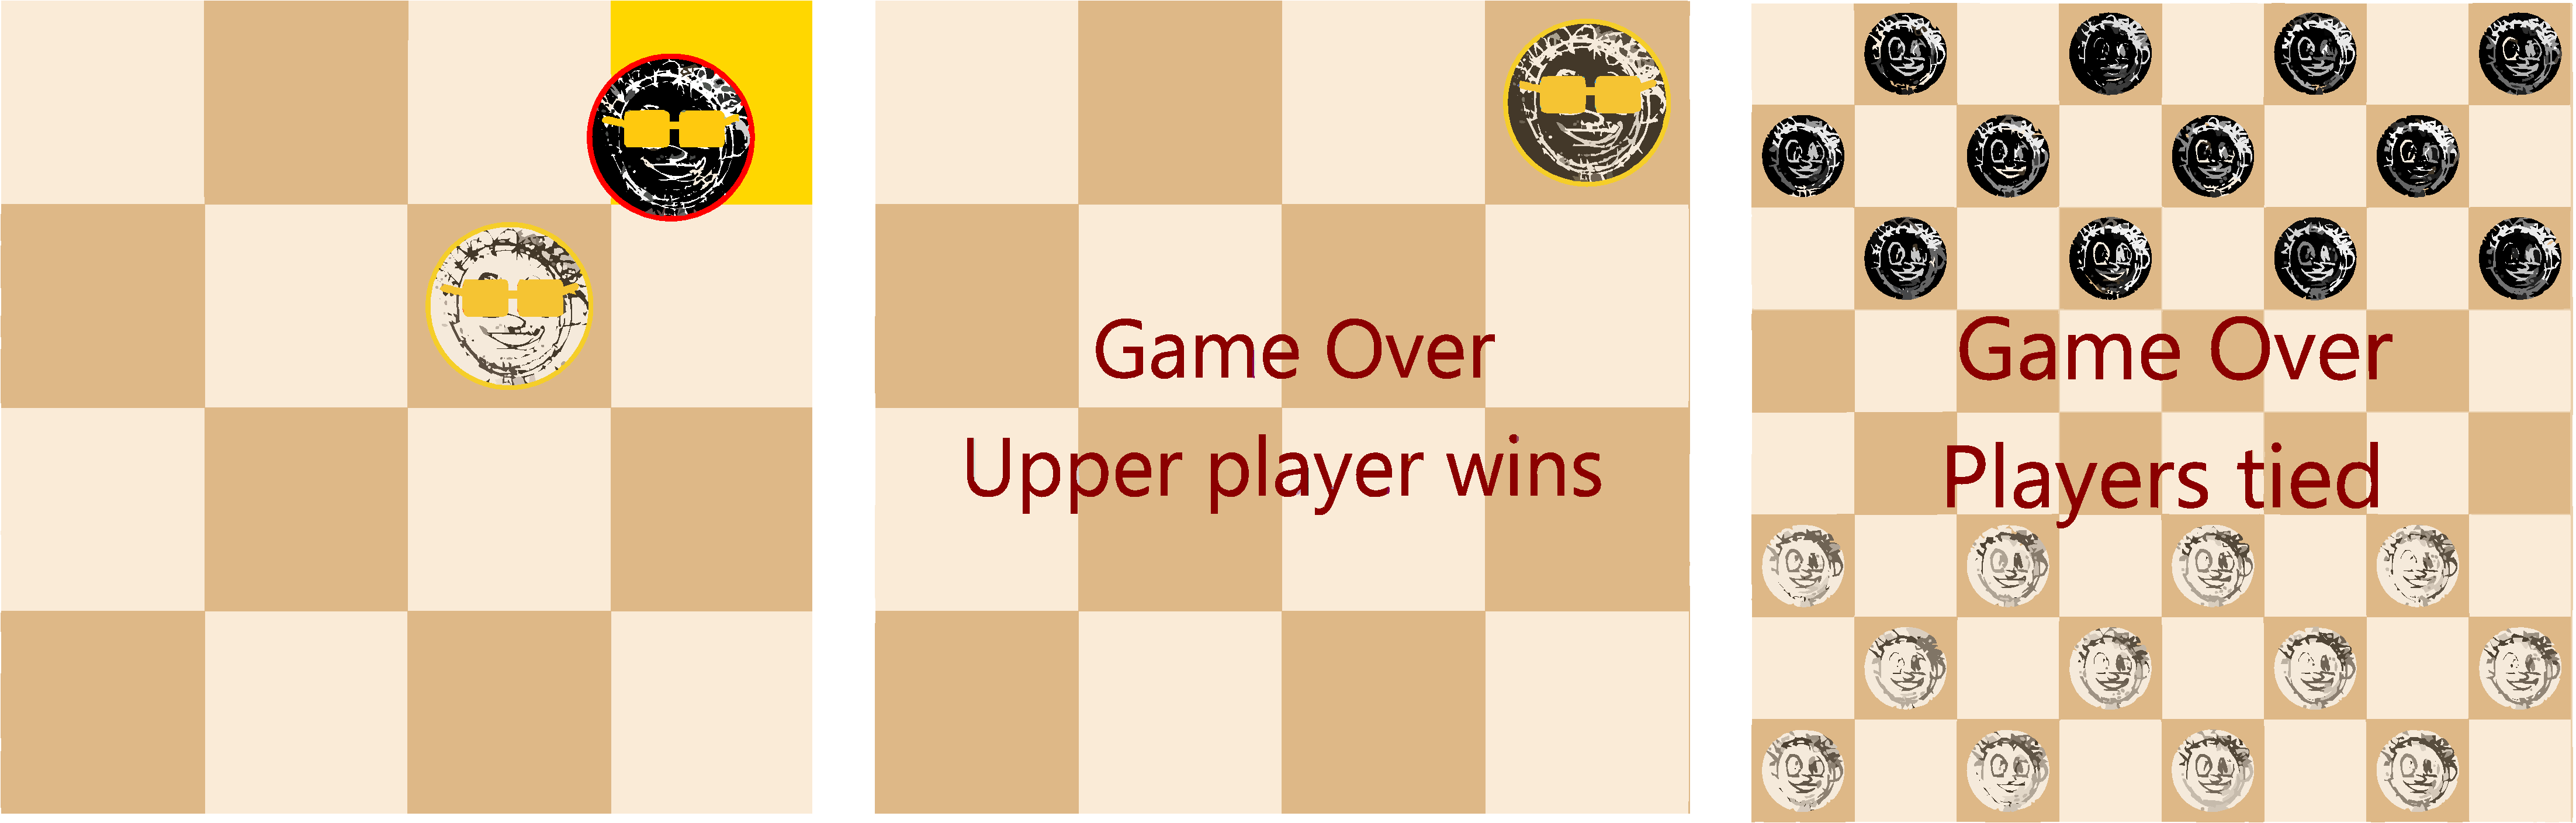
\includegraphics[width = 1.0 \textwidth]{Figurer/gameOverWinTie.pdf}
        \caption{Her kan det ses hvordan et spil afsluttes. Spillet er ovre hvis en spiller er løbet tør for brikker, hvis en spiller ikke kan flytte en brik, eller hvis begge spillere vælger at sige uafgjort spil.}
        \label{fig:gameOverWin}
    \end{figure}

\textit{Uafgjort:} I \texttt{gameScene} er der to knapper i form af \texttt{CheckBox upperTieCheckBox} og \\
\texttt{bottomTieCheckBox}. Disse har hver en listener, der, når de bliver hakket af, tjekker om begge check boxes er blevet hakket af. Hvis dette er sandt, køres metoden \texttt{gameOver}. \texttt{gameOver} laver en label, indeholdende tekst afhængig af hvordan spillet blev sluttet. Denne label bliver sat ind i \texttt{damModel}, og derefter sættes \texttt{playerThisTurn} til \texttt{None}, hvilket gør at ingen spiller kan tage deres træk. \\

%   RR
%    \item Hvordan er save og load implementeret?
%    \item Hvordan lagres data i en save file? 
%    \item Hvordan forhindres fejl loading? (load uden save file) 
\textbf{Save og load:} 
Save og load bruger hovedsageligt \texttt{Serializable} og klasserne \\
\texttt{ObjectOutputStream}/\texttt{ObjectInputStream}. Klassen \texttt{ResourceManager} håndterer selve det at gemme og hente filerne ved brug af det givne filnavn i strengen \texttt{"filename"}. Data om modellen, der skal gemmes, lagres i \texttt{ModelData}. Dvs.: de anvendte indstillinger og brikkerne på brættet. Da brikkerne nedarver \texttt{Ellipse} er de ikke \texttt{Serializable}, så de konverteres ved brug af klassen \texttt{PieceData}. \texttt{PieceData} indeholder brikkens position, spiller og om den er kronet. \\

Når brikkerne er gemt via \texttt{PieceData} og spillet er gemt i \texttt{ModelData}, gemmes det i en lokal fil med navnet \texttt{"Checkers.sv"}. Den gemte fil bliver gemt uden for \texttt{.jar} filen ved brug af klassen \texttt{ObjectOutputStream}.\\

Hver gang spillet startes bliver der tjekket om en legal gemt fil findes i samme directory hvilket bestemmer om \texttt{"Load"} knappen er aktiv eller ej. Så snart man trykker på \texttt{"Save"} vil load blive aktiv igen, da det så er sikkert at filen er legal. \\

Den eneste måde at prøve at loade en illegal fil på er ved at have spillet kørende imens man ændrer i den gemte fil, og så prøve at loade den. På den måde er filen ikke blevet tjekket inden den hentes, men vil da blive fanget i en \texttt{try-catch} og stoppet. Hvis man prøver at hente illegal en fil, vil knappen \texttt{"Load"} kunne klikkes, men den vil ikke gøre noget; fejlen fanges med en \texttt{try-catch}.
\subsubsection{AI}

Vi har implementeret en kunstig intelligens som modstander. AI'en aktiveres gennem menuen. \\

% Magnus
% Hvordan animeres flytning af brik? (adv, begge?)
\textbf{Animation af flytning af brik:} Når AI foretager et træk, er animationen vha. \texttt{JavaFX}'s \texttt{TranslateTransitions} i \texttt{AI}. Først oprettes et objekt af typen \texttt{TranslateTransition}. Derefter tilknyttes den en shape, der skal translateres (flyttes). Start- og slutkoordinaterne på skærmen markeres i view koordinater, relativt til den nuværende position. Endeligt sættes den tidslige varighed af flytningen, og bevægelsen sættes igang. \\

%   RR
%    \item Hvordan animeres AI flytning af comboer?
\textbf{Comboer:} 
Eftersom AI'en simulerer en bruger, har den samme muligheder og indstillinger som en bruger. Hvis indstillingen \texttt{"Combos must be completed"} er sat til, vil AI'en også udføre comboerne. Animationen for denne handling er dog ikke helt optimal. De dræbte brikker animeres væk, men animationen går direkte fra startposition til slutposition. \\

%   RR
%    \item Hvor mange ressourcer bruger AI?
\textbf{AI's brug af ressourcer:} Den implementerede AI finder en tilfældig brik, der kan flytte, og flytter denne brik til et tilfældigt legalt felt. Hvis den kan dræbe, foretager den et drab. Med denne implementering bruger AI'en samme regnekraft, som hvis brugeren skulle foretage et træk. Det gør, at der ikke er nogen bemærkelsesværdig forsinkelse i spillet, der spilles mod AI.

\section{Evaluering}
%\input{Evaluering/Evaluering.tex}
\subsection{Overordnet}\label{sec:evaOverordnet}

% Magnus
\textbf{Møder på DTU:} Gruppen har mødtes dagligt, både i planlægnings-, implementerings- og rapportskrivningensfasen. Den første uge brugte vi en storskærm i 324, så alle kunne følge med i den grundlæggende kodes tilblivelse linje for linje. \\

% Magnus
% Hvordan holdt I styr på projektet?  Logbog.
\textbf{Logbog:} For at holde styr på projektets status, har vi ført logbog flere gange dagligt i \texttt{Google Docs}. Logbogen er nu på 10 sider, og rummer oversigter over: Hvad er for nyligt blevet implementeret eller debugged? Hvad skal implementeres eller debugges fremover? Logbogen benytter også farvekoder; Features der skal implementeres er farvet rød. Når de er implementeret, farves de grønne. Vi har også noteret når fx metoder skifter funktionalitet, eller variable har fået nyt navn for at øge læsbarheden af koden.\\

\begin{figure}[H]
\centering
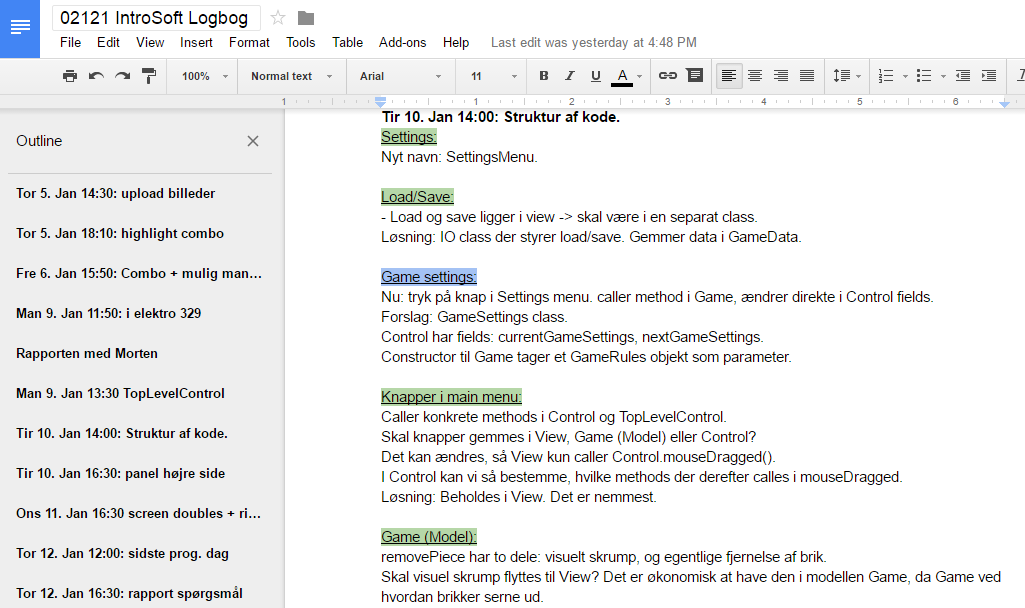
\includegraphics[width = 0.7  \textwidth]{Figurer/logbog.png}
\caption{Udsnit af den brugte logbog i løbet af projektet. Logbogen indeholder ting der skulle huskes, ting der er blevet implementeret, eller ideer til fremtidige implementeringer til programmet.}
\label{fig:logbog}
\end{figure}

% Magnus
\textbf{Sammenligning med andres spil:} For at få overblik over, hvad der adskiller vores program fra de andre gruppers, har vi besøgt andre grupper og spillet deres spil. De har spillet vores spil, og vi har spillet deres. Vi har stillet dem spørgsmål om implementering, og de har stillet os spørgsmål. Svarene på deres spørgsmål er inkorporeret i rapporten. \\

% Magnus
\textbf{100 spørgsmål:} For at sikre, at vi fik forklaret alle væsentlige dele af programmets design og implementering, stillede vi 100 spørgsmål, fx: Hvordan flytter spilleren en brik? Hvordan ændres brætstørrelsen? Hvordan highlightes felter?
Vi tog derefter udgangspunkt i, at rapporten skulle besvare alle spørgsmål. På den måde forsøgte vi at dokumentere programmet fyldestgørende. 
\subsection{\textsc{SimpDam}}\label{sec:evaSimp}

%   RR
%   \item Debugging: Hvor sikkert er spillet? Hvilke sanisations har I på inputs?
\textbf{Program sikkerhed:} Vi har indført sanitering for brikkers position, så de ikke kan trækkes udenfor brættet. Når en brik bliver sluppet over et felt, tjekkes hvorvidt flyttet er lovligt via metoderne i figur \ref{fig:tjekliste}. Når brætstørrelsen vælges (mellem 3 og 100), håndteres inputtet via \texttt{try-catch}. 


\subsection{\textsc{AvaDam}}\label{sec:evaAva}

%   RR
%   \item Debugging: Hvor sikkert er spillet? Hvilke sanisations har I på inputs?
\textbf{Program sikkerhed:} 
Når det kommer til sanitering af input, er programmet simpelt. Der er få bruger inputs; indstillinger sættes gennem checkboxes. Brætstørrelsen vælges via en slider; det gør sanitering unødvendig. Ved upload at billeder har vi tilføjet et filter, der kun gør det muligt at vælge billedtyper accepteret af \texttt{JavaFX}'s \texttt{ImagePattern}. Ved load og save køres default filstier, og der kan ikke loades ugyldige save filer. \\

%   RR
%    \item Hvordan endte I med den program struktur, I har? (historie om highlights)
\textbf{Programstruktur:} 
Strukturen af programmet er blevet ændret i løbet af projektet. En af de største og mest markante ændringer var, da vi gik fra at \textit{verificere} et træk til at \textit{forudsige} legale træk. Da vi indførte highlighting til \texttt{Control}, blev implementeringen af combo simplificeret.  \\

\textit{Før:} Først finder vi legale slutfelter (tjek 1). De blev highligted. Derefter slap vi en brik på et felt, og tjekkede derefter, om det var legalt at slippe brikken her, på samme måde som i \textsc{SimpDam} (tjek 2).\\

\textit{Nu:} Først finder vi legale slutfelter. Så slipper vi en brik. Hvis slutfeltet er highlighted, er feltet en legal destination, så brikken må selvfølgelig slippes her. Det kræver kun ét tjek!\\

% Roar
\textbf{AI:} Der var foretaget to forskellige indfaldsvinkler til vores AI. Den første og simpleste var en tilfældig AI. Denne fandt en tilfældig brik der kunne flytte, og flyttede den et tilfældigt legalt sted hen. \\

Vi prøvede også med en AI der ikke tog et tilfældigt legalt træk, men som gav alle felter en værdi.
Værdien var et udtryk for, hvor taktisk feltet var at lande på. Da en optimal strategi umiddelbart ikke kan generaliseres, blev vægtningen af omgivelserne skabt ved en evolutionær algoritme, der bruge princippet bag q-learning. \\

Selvom vægtningerne blev indstillet automatisk, skulle man stadig forudbestemme hvilke parametre der blev brugt på hvilke felter i beregningerne, hvilket gjorde implementeringen til en større udfordring, end hvad der var tid til. Den brugte AI er dermed den første, selvom det var spændende at prøve med andre tilgange.  \\

%   RR
%    \item Hvad ville I implementere/debugge/forfine, hvis I havde mere tid? 
\textbf{Mulige implementeringer/ændringer:} 
Nogle af de features vi gerne ville tilføje til / ændre i programmet, men ikke nåede pga. tid er:

\begin{enumerate}
\item Bedre animation af AI combo.\footnote{ En mere optimal måde at gøre det på, ville være at animere flytningen af comboen selv. Dette ville umiddelbart kunne indføres uden større besvær. En eventuel implementering ville være at bruge \texttt{PathTransition} og positionerne i \texttt{comboPositions} fra \texttt{Control.}}
\item Uafhængighed i model-view-control designmønstret.
\item Musik og lyde.
\item Anden AI.
\item Custom bræt (huller og piedestaler)
\item Bonus effekter.
\item Power-ups.
\item Hexagonale felter.
\end{enumerate}


% Magnus
\section{Konklusion}
\textbf{Afgrænsning:} Målet med dette projekt var at designe og implementere et computerspil baseret på det klassiske brætspil dam. Med udgangspunkt i reglerne fra Dansk Dam Forening designede og implementerede vi først et simpelt spil \textsc{SimpDam}, og udvidede derefter \textsc{SimpDam} med til \textsc{AvaDam} ved at tilføje en række features. De tilføjede features blev præsenteret i afsnit \ref{sec:afgraensning}.\\

\textbf{Design:} I afsnit \ref{sec:designMVC} redegjorde vi for, hvordan vores designmønster tog udgangspunkt i model-view-control. I afsnit \ref{sec:designSimpDam} gjorde vi rede for hvordan brætstørrelsen ændres i \textsc{SimpDam} gennem terminalen eller konsollen. I afsnit \ref{sec:designAvaDam} gennemgik vi hvordan brætstørrelse og aktiverede regler ændres i \textsc{AvaDam} gennem menuerne, hvordan brugervejledningen er implicit i spillet gennem visuelle indikatorer, og hvilke features vi havde indført for at gøre spillet underholdende: tilpasselige brik-billeder, AI og animationer af brikbevægelser. \\

\textbf{Implementering:} I afsnit \ref{sec:ImpOverordnet} dokumenterede vi hvordan \textsc{SimpDam} og \texttt{AvaDam} er implementeret med \textsc{JavaFX}, hvordan vi anvendte static fields og metoder, og hvordan navngivningen af fields og metoder er anvendt i vores kildekode. 
I afsnit \ref{sec:ImpSimp} og \ref{sec:ImpAva} gennemgik vi spillets anvendte klasser, hvordan brættet og brikkerne lagres og opdateres, og i detaljer hvordan de tilføjede features er implementeret i \textsc{AvaDam}.\\

\textbf{Evaluering:} I afsnit \ref{sec:evaOverordnet} gav vi et indblik i hvordan vi som gruppe strukturerede projektet internt, og hvordan vi fik erfaring eksternt ved at udveksle spørgsmål og teste andre gruppers spil. I afsnit \ref{sec:evaSimp} og \ref{sec:evaAva} sammenlignede vi \textsc{SimpDam}s og \textsc{AvaDam}s sikkerhed.  Endeligt præsenterede vi de tilføjelser og ændringer, vi ikke nåede i dette projekt. \\

\textbf{Afsluttende} kan vi konkludere, at selvom vi sagtens kunne have brugt en uge mere, er projektet  lykkedes: Vi  har designet og implementeret et simpelt dam brætspil. Igennem projektet er vi blevet bedre til at organisere, planlægge og udføre samarbejde i en projektgruppe, og anvende softwareredskaber som \texttt{Java} og \texttt{JavaFX}.


\section{Gloser}
\label{Gloser}
\begin{itemize}
\item \textbf{Kombinationsdrab/Combo:} I koden og rapporten refererer et kombinationsdrab (eng; combo) til et træk hvor en spiller tager én eller flere af fjendens brikker, eller til selve aktionen hvor én brik bevæger sig over og tager flere af modstanderens brikker. Læg mærke til at et enkelt \textit{kill} i koden også er en combo.
    
\item \textbf{Drab/Kill:} I koden og rapporten refererer et kill (dansk; drab) til et træk hvor en spiller tager én af modstanderens brikker, eller til selve aktionen hvor én brik bevæger sig over og tager en af modstanderens brikker. 
    
\item \textbf{Valgt brik/Selected piece:} I koden og rapporten refererer en valgt brik til den brik der er i færd med at blive trukket af musemarkøren. 

\item \textbf{Field:} I rapporten refererer et field til et field i \texttt{Java}.

\item \textbf{Felt:} I rapporten refererer et felt til et felt på brættet, altså et \texttt{Tile}.

\item \textbf{Highlight:} I koden og rapporten refererer det at highlighte et felt til at ændre dens farve, for at markerer at det er et gyldigt træk at flytte hen til den.

\end{itemize}

%760,000 BADNESS

%\begin{figure}[H]
%\centering
%
\includegraphics[width = 0.75\textwidth]{maaikkeslettes}
%\caption{I'ma shit in your mouth when u sleepz}
%\label{fig:my_label}
%\end{figure}

\end{document}
